%\documentclass[12pt,a4paper,twoside,openright,draft]{book}
\documentclass[12pt,a4paper,twoside,openright]{book}

% Margini delle pagine
\setlength{\oddsidemargin} 		{2. cm}
\setlength{\evensidemargin} 	{2. cm}
\addtolength{\oddsidemargin} 	{-0.4 cm}
\addtolength{\evensidemargin} {-0.4 cm}

% Interlinea
\linespread{1.1}

% Rientro della prima riga del paragrafo
\setlength{\parindent}{0.5cm}

% Pacchetti da utilizzare
\usepackage[italian]{babel}																		% Sillabazione in italiano
\usepackage[latin1]{inputenc}																	% Encoding con lettere accentate
\usepackage{amsmath}																					% Simboli matematici
\usepackage{graphicx}																					% Figure
\usepackage{hyperref}																					% Link interni clickabili
\usepackage{subfigure}																				% Per avere pi� figure ``unite''
\usepackage{lscape}																						% Per avere tabelle o figure ruotate
\usepackage[margin=20pt, font=small, labelfont=bf]{caption}		% La descrizione di figure e tabelle
\usepackage{fancyhdr}   																			% Per modificare l'header delle pagine
\usepackage[version=3]{mhchem} 																% Formule chimiche
\usepackage{methylen,aliphat,carom,hetarom,chemist,epic}			% Formule chimiche
\usepackage{enumerate}

% ======================= Modifiche per l'header =================================
% Modifica lo stile della pagina secondo le specifiche del pacchetto fancy
\pagestyle{fancy}

% Modifica l'header delle pagine secondo lo stile fancy
\fancyhead{}

% Altezza dell'header
\renewcommand{\headheight}{15pt}

% Spessore della riga sotto l'header
\renewcommand{\headrulewidth}{0.4pt}

% Contenuto dell'header
\renewcommand{\chaptermark}[1]{\markboth{\chaptername\ \thechapter\ -\ \emph{#1}}{}}
\fancyhead[RO,LE]{\leftmark}
% =================================================================================

% Informazioni che vengono inserite come descrizione del PDF prodotto.
\hypersetup{
	pdftitle = {Chimica indistriale II},
	pdfsubject = {Appunti del corso tenuto da E. Tronconi al Politecnico di Milano},
	pdfkeywords = {chimica industriale, sintesi, prodotti},
	pdfauthor = {\textcopyright\ Marco Vito Moscaritolo},
	pdfcreator = {\LaTeX},
	pdfproducer = {pdfeTeX-0.\the\pdftexversion\pdftexrevision},
	bookmarksnumbered = true,
	bookmarksopen = true,
}

% Imposta il colore dei link.
\hypersetup{colorlinks=true,
						linkcolor=magenta,		% Colore dei link interni al documento
						anchorcolor=magenta,	% Colore dei link ad ancore
						citecolor=magenta,		% Colore dei link a fonti bibliografiche
						filecolor=magenta,		% Colore dei link a file locali
						menucolor=magenta,		% Colore dei link nel menu di adobe Acrobat Reader
						urlcolor=magenta,			% Colore dei link a url
					 }

% Rende bianche le pagine di fine capitolo		
\makeatletter
	\def\cleardoublepage{\clearpage\if@twoside \ifodd\c@page\else
  	\hbox{}
    \thispagestyle{empty}
    \newpage
    \if@twocolumn\hbox{}\newpage\fi\fi\fi}
\makeatother

%
% Argomento 1:
% Materie prime dell�industria chimica organica. Gas naturale e sue linee produttive. 
% Metanolo. Acido acetico.
%
% Argomento 2: 
% Petrolio. Processi di raffineria: topping, reforming catalitico, cracking termico e 
% catalitico, visbreaking, coking, hydrotreating.
%
% Argomento 3:
% Il petrolio come fonte di materie prime per l�industria chimica organica. Olefine da 
% steam cracking; separazione della frazione C4. Aromatici: separazione aromatici / 
% alifatici; frazionamento degli aromatici C8.
% 
% Argomento 4:
% Esempi di processi petrolchimici per la produzione di monomeri. Processo bilanciato 
% per la produzione di VCM da etilene e cloro. Processi per la produzione di anidride
% maleica da benzene e da butano.
%
% Argomento 5:
% Sintesi industriale di polimeri. Polimerizzazione del VCM a PVC.
%

% Documento da produrre ================================================
\begin{document}
% Frontespizio =========================================================
  \frontmatter
		\thispagestyle{empty}

\vspace*{-1.5cm} 

\begin{center}
  \large
  POLITECNICO DI MILANO\\
  \normalsize
  Corso di Laurea in Ingegneria Chimica\\
  Dipartimento di Chimica e dei Materiali "Natta"
  
  \vspace*{3cm} 
  
  \LARGE
  \textbf{Chimica Industriale II \\ Chimica Industriale Organica}
  
  \vspace*{1.5cm}
  
  \normalsize
  Prof: Enrico Tronconi
\end{center}
\vspace*{6.0cm}
  
\begin{flushright}
\begin{table}[h]
		\begin{tabular}{p{5cm}ll}
			& Appunti di: 	&  Marco Vito Moscaritolo \\ 
			& Mail: 				& \href{mailto:mavimo@gmail.com}{mavimo@gmail.com} \\
			& Website: 			& \href{http://mavimo.netsons.org}{http://mavimo.netsons.org}
		\end{tabular}
\end{table}
\end{flushright}

\vspace*{0.5cm}
\begin{center}
	Anno Accademico 2005-2006
\end{center}
\clearpage

\begin{figure*}
	\centering
		\includegraphics{image/CCsomerights.pdf}
	\label{fig:CCsomerights}
\end{figure*}

\small
\noindent Il contenuto di questo documento � distribuito secondo la:
\begin{center}
	\Large
	\textbf{Creative Commons Licence v 2.5}\\
	\small Attribuzione - Non commerciale - Non opere derivate
\end{center}

\vspace{1cm}

\noindent Potete trovare il testo completo della licenza al seguente link:\\
\begin{center}
\url{http://creativecommons.org/licenses/by-nc-nd/2.5/it/}
\end{center}

\vspace{3cm}

\normalsize
\noindent Versioni precedenti:

\small
\begin{itemize}
	\item 0.1.0 - 20/08/2006 - Sintesi del metanolo
	\item 0.2.0 - 24/08/2006 - Sintesi dell'acido acetico
	\item 0.3.0 - 28/08/2006 - Sintesi del cloruro di vinile
	\item 0.4.0 - 31/08/2006 - Sintesi dell'anidride maleica
	\item 0.5.0 - 31/08/2006 - Gas naturale come materia prima
	\item 0.6.0 - 27/04/2007 - Revisione di quanto presente
	\item 0.8.0 - 20/06/2007 - Aggiunta della parte relativa al petrolio
	\item 0.8.5 - 22/06/2007 - Sintesi dell'MTBE
	\item 0.9.0 - 01/09/2007 - Revisione di quanto presente
\end{itemize}

% Indice ===============================================================
		\tableofcontents
		
% Capitoli =============================================================
	\mainmatter
	 \chapter{Introduzione alla chimica organica}

	 \chapter{Gas naturale (\textit{NG})}
Il gas naturale � una materia prima alternativa a petrolio, soprattutto nella produzione di idrogeno e di gas di sintesi (una miscela di $H_2$ e $CO$) mediante steam reforming. \'E costituito prevalentemente da metano ($CH_4$), ma pu� contenere anche frazioni significative di paraffine ($C_2$ e $C_3$). In base al quantitativo di condensabili ($C_2$ e $C_3$) presenti si distingue in \textit{dry gas} e \textit{wet gas}, inoltre se la presenza di $CO_2$ e $H_2S$ � significativa il gas si dice \textit{acido}.

Il gas naturale si pu� trovare in giacimenti associato al petrolio, nel qual caso i costi di estrazione sono minimi, mentre per i pozzi di \textit{NG} non associati i costi sono maggiori, poich� non vi sono materie di maggior pregio da estrarre con esso.

\section{Purificazione}
La purificazione del metano da $H_2S$ pu� essere svolta usando un assorbimento chimico o fisico. L'assorbimento \textit{chimico} viene scelto quando le quantit� di acido solfidrico da rimuovere sono basse, mentre per grandi quantitativi di acido da asportare si utilizza l'assorbimento \textit{fisico}.

L'assorbimento chimico viene condotto in colonne di assorbimento, alla cui base viene inviato il gas da trattare, mentre dalla testa si inviano soluzione alcaline di etanolammine o carbonato di potassio ($K_2CO_3$). \'E un trattamento altamente selettivo, ma se il quantitativo di acido solfidrico � troppo elevato si ha saturazione del solvente con conseguente perdita di attivit�.

L'assorbimento fisico viene preferito quando si hanno elevate quantit� di gas da trattare con elevate concentrazioni di $H_2S$. L'operazione viene condotta in una colonna di assorbimento e il solvente � costituito da \textit{N-metil-pirrolidone} glicoli e metanolo. L'utilizzo di questi solventi da una minore selettivit�, ma al contempo non ha problemi di saturazione del solvente. La fase successiva del processo � la rigenerazione del solvente in un colonna di stripping.

Sono possibili anche purificazioni tramite assorbimento ossidativo a zolfo (adatto a piccole correnti da trattare) o assorbimento su letti solidi (costituiti da ossidi di ferro, zinco o carboni attivi), che per� devono essere rigenerati.

In tutti questi casi il gas naturale viene trattato in pressione in modo da favorire il fenomeno di assorbimento, con scelta del meccanismo in base alla portata e alla concentrazione dei gas, come visibile in \figurename~\ref{fig:NG:Adsorbimento}

\begin{figure}[htbp]
	\centering
		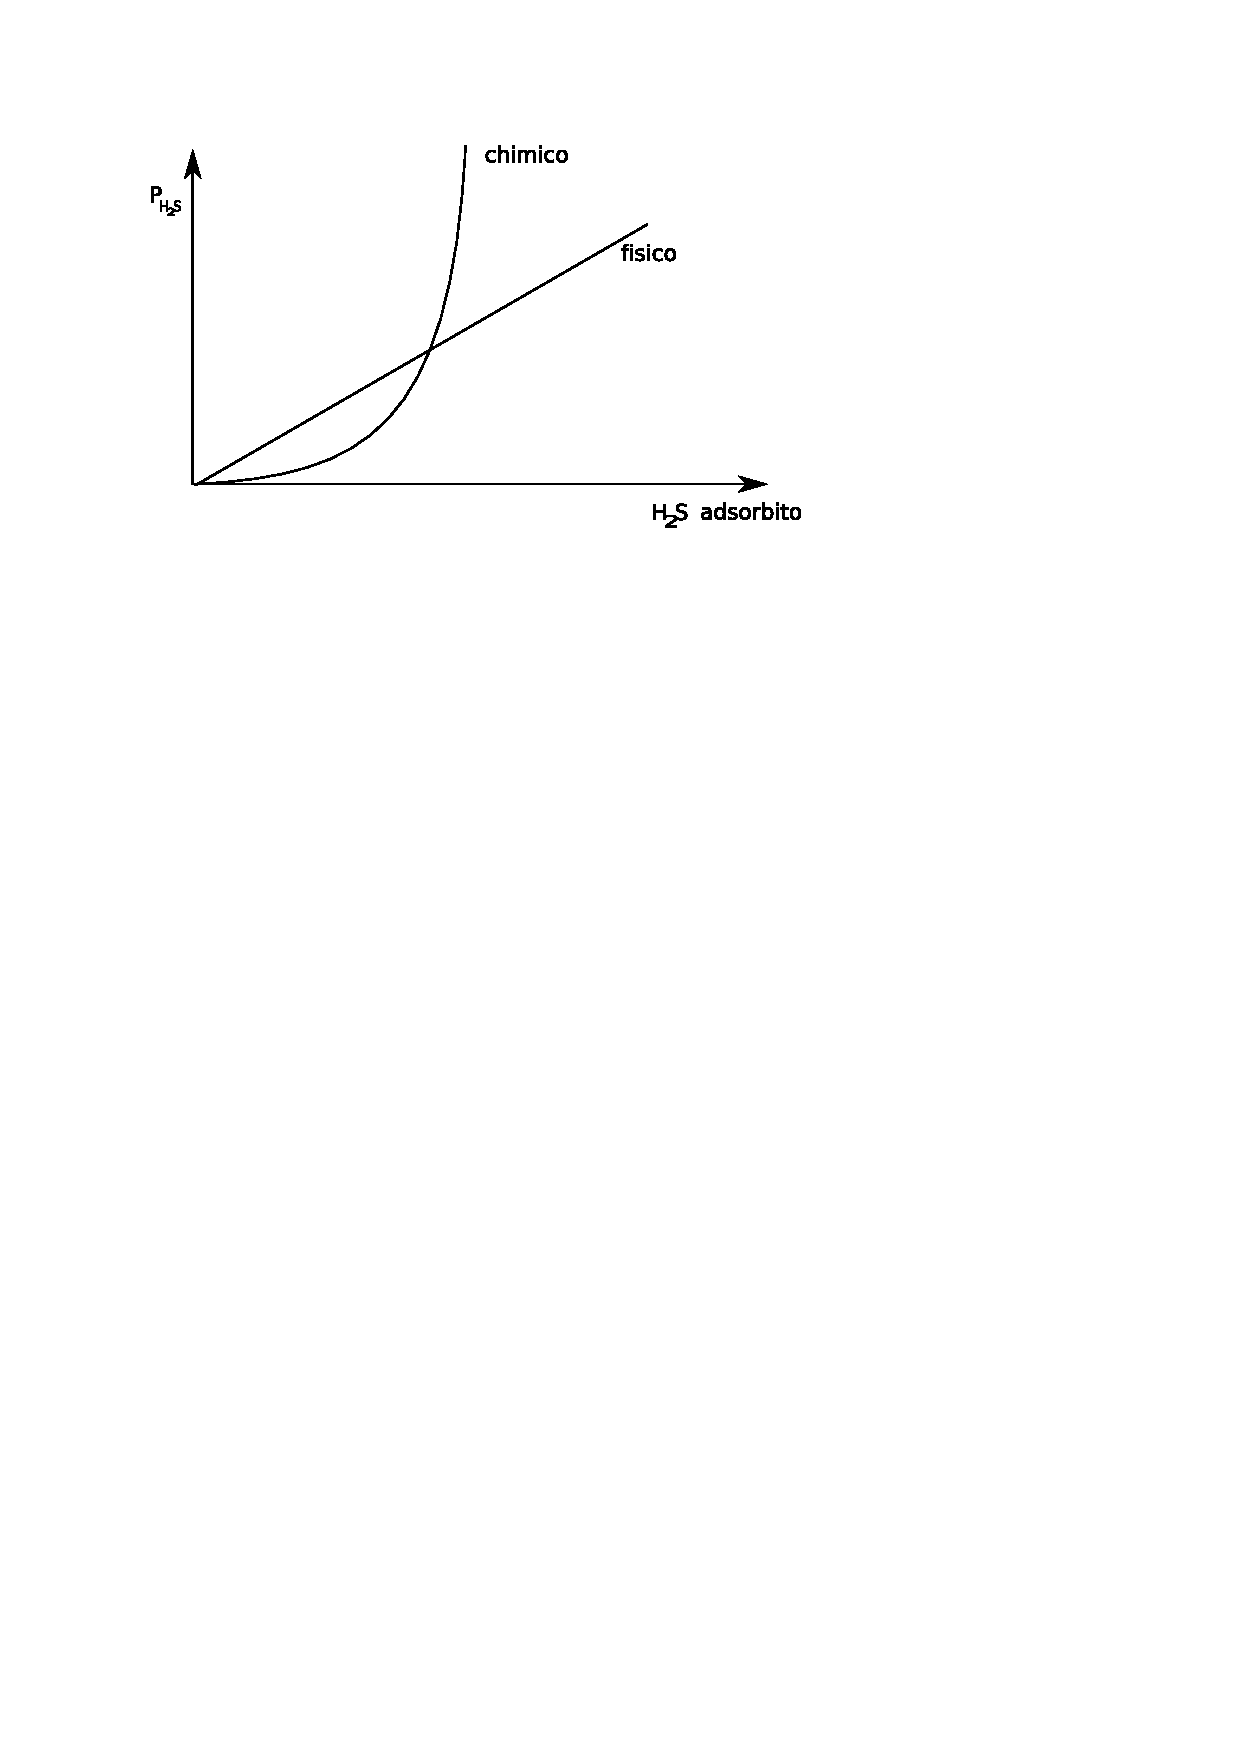
\includegraphics[width=0.60\textwidth]{image/NGAdsorbimento.pdf}
	\caption{Confronto tra assorbimento \textit{chimico} e \textit{fisico} a diverse concentrazioni di $H_2S$}
	\label{fig:NG:Adsorbimento}
\end{figure}

\section{Trasporto}
Il trasporto del gas naturale dal punto di estrazione ai punti di consumo pu� essere effettuata tramite gasdotti o, una volta liquefatto, con navi metaniere. Attualmente il 75\% del \textit{NG} viene trasportato per mezzo di gasdotti, in cui il gas si trova a una pressione di circa 80MPa, mentre il restante viene trasportato via mare.

La scelta del tipo di trasporto da effettuare dipende, tanto dalle infrastrutture presenti nel luogo di estrazione (presenza o meno di gasdotti), quanto dalla distanza da percorrere, infatti per liquefare il gas naturale � necessario portarlo (e conservarlo) a una temperatura di circa -160�C, con un costo energetico di circa 6MJ/kg. Il metodo di scelta del tipo di trasporto pu� ben essere rappresentata in \figurename~\ref{fig:NG:Trasporto}. Come � evidente le spese per il trasporto su \textit{pipeline off-shore} (fuori costa, in mare) crescie pi� rapidamente che non il trasporto \textit{on-shore}.

\begin{figure}[htbp]
	\centering
		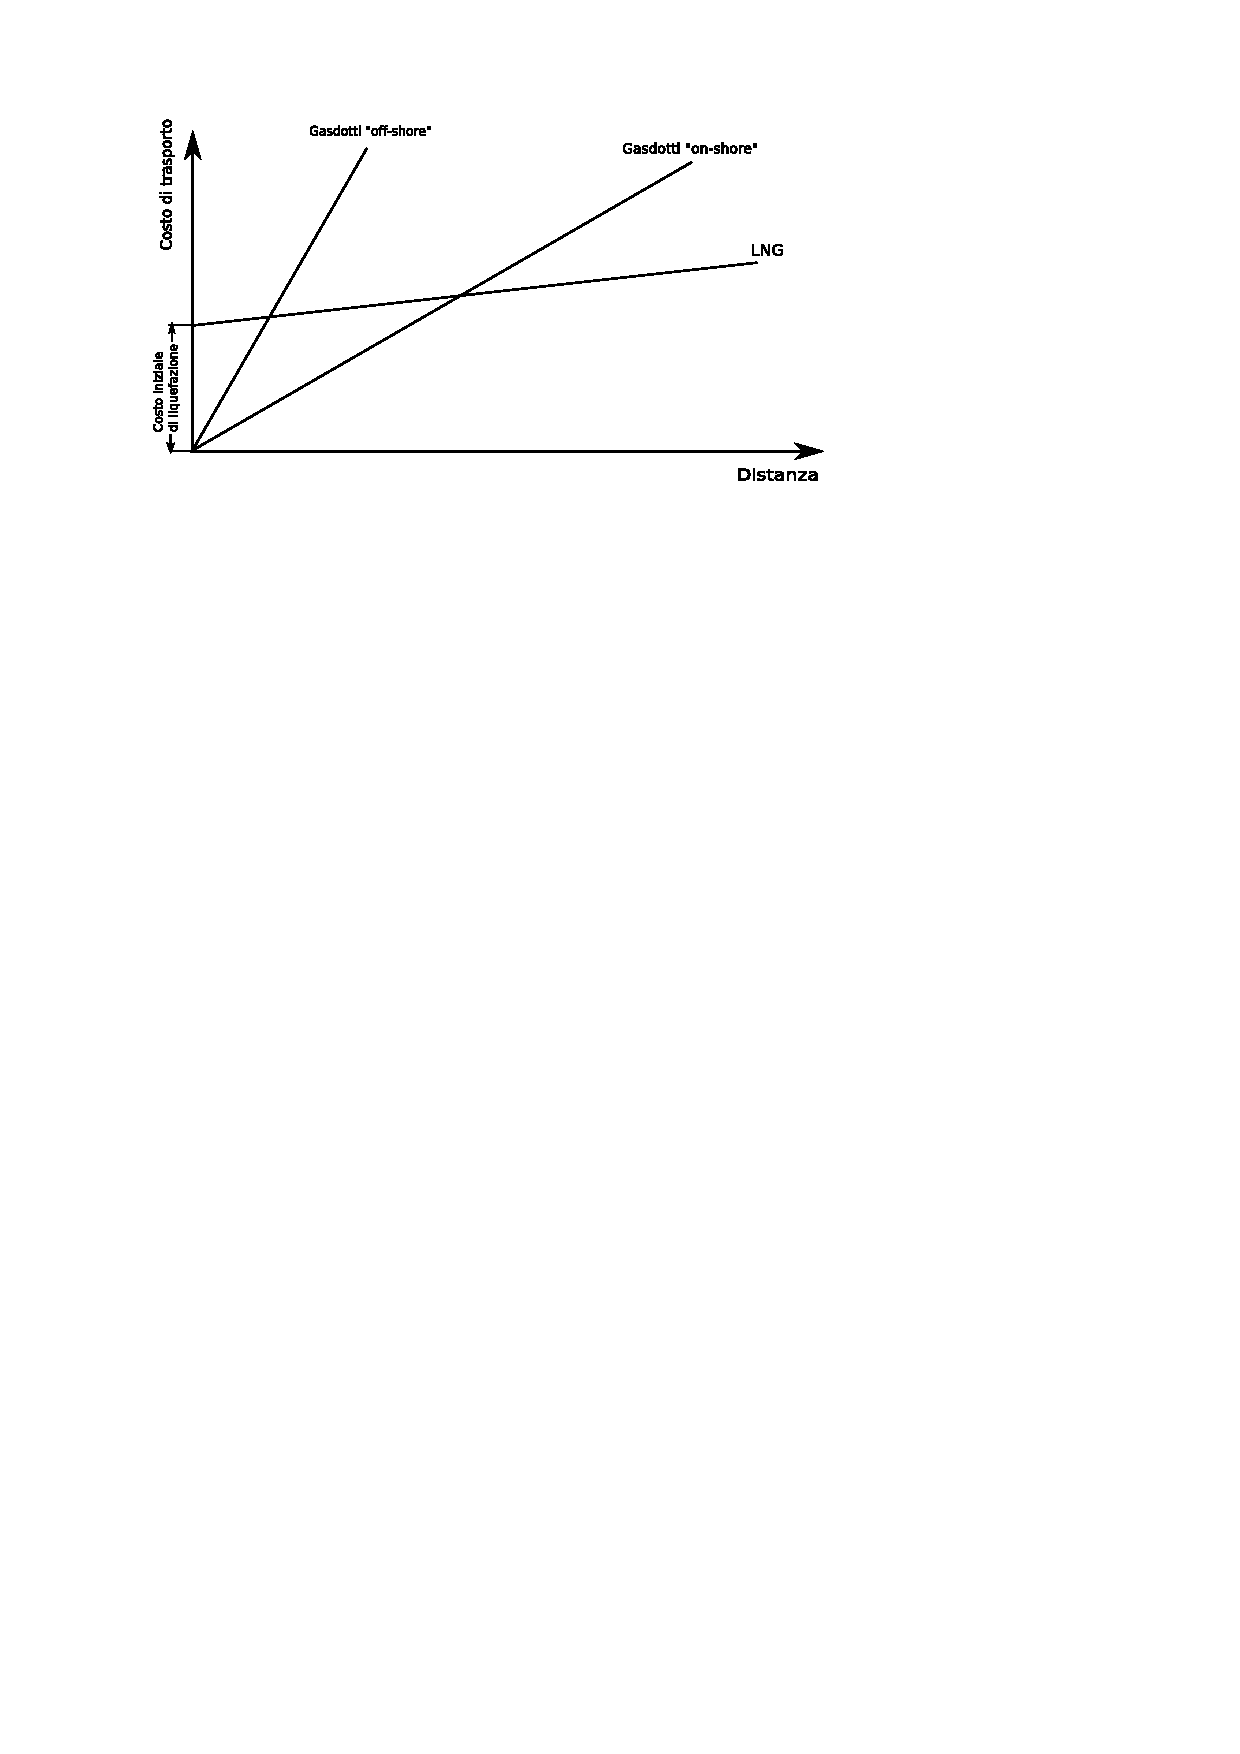
\includegraphics[width=0.60\textwidth]{image/NGTrasporto.pdf}
	\caption{Costo per le diverse tipologie di trasporto in funzione della distanza}
	\label{fig:NG:Trasporto}
\end{figure}

Il quantitativo di \textit{NG} trsporto su navi metaniere � di circa $125000m^3$, in cui il metano � stoccato a -160�C in forma liquida ($d = 424kg/m^3$) con una concentrazione circa 600 volte maggiore che il gas allo stato gassoso; la portata nei gasdotti � di $2-4 \cdot 10^6 Nm^3/h$.

Un'alternativa al trasporto del gas naturale in altri siti � l'utilizzo in loco per la produzione di metanolo che costitusce un prodotto di maggior pregio ed � pi� facilmente trasportabile.
	 \chapter{Sintesi del Metanolo}

\section{Caratterisitche chimico-fisiche}
Temperatura di fusione = -98�C (175K)\\
Temperatura di normal ebollizione = 64.6�C (337.5K)\\
Solubile in acqua\\
Tossico\\
Limite di esplosivit� inferiore (in aria) = 6.7\% (v\/v) \\
Limite di esplosivit� superiore (in aria) = 36.5\% (v\/v)

\section{Principali impieghi}
La produzione mondiale annua del metanolo si aggira nell'intorno di $10^6$ tonnellate annue, come riportato in \tablename~\ref{tab:MetOH:ProduzioneAnnua}.
\begin{table}[htbp]
	\centering
		\begin{tabular}{p{1.8cm}p{1.8cm}p{1.8cm}p{1.8cm}p{1.8cm}p{1.8cm}}
			Anno	& Mondo	& USA		&	Canada 	& Europa occidentale & Giappone \\ \hline
			1978	& 12		& 3.4		&					&	3			&	1			\\
			1979	& 15		& 4.05	&					&	3.45	&	1.35	\\
			1980	& 			& 			&					&	2.5		&				\\
			1981	& 8			& 			&					&				&				\\
			1983	& 15.9	& 5.52	&	1.75		&	2.53	&	1.27	\\
			1988	& 			&	 			&	1.81		&				&				\\
			1989	& 19		& 			&					&				&				\\	
			1990	& 22.3	& 			&					&				&				\\
			1991	& 22.1	& 4.42	&	2.21		&	2.65	&	0.22	\\
			1992	& 			& 3.66	&	2.15		&				&	0.077	\\
			1993	& 			&	4.78	&					&				&	0.034	\\
			1995	& 30.1	& 			&					&				&				\\ \hline
		\end{tabular}
	\caption[Produzione annua di metanolo tra il 1978 e il 1995.]{Produzione annua di metanolo tra il 1978 e il 1995 ($\times 10^6$ tonn/anno).}
	\label{tab:MetOH:ProduzioneAnnua}
\end{table}

I principali utilizzi di questo prodotto sono elencati in \tablename~\ref{tab:MetOH:Utilizzo} ed evidenziano il cambiamento dell'impiego verso la produzione di \textit{MTBE} a seguito delle scelte di sostituire il \textit{piombo-tetraetile}, fino ad allora usato come antidetonante per benzine, con questo prodotto.
\landscape
\begin{table}[htbp]
	\centering
		\begin{tabular}{lp{1.95cm}p{1.95cm}p{1.95cm}p{1.95cm}p{1.95cm}p{1.95cm}p{1.95cm}}
		  Prodotto 						& Mondo	& Mondo	& USA	 & USA	& Giappone & Europa 
		  																																occidentale & Brasile \\
      										& 1979	& 1988  & 1973 & 1985 & n.g.     & 1985         & n.g.  \\ \hline
     Formaldeide 					&    52 & 40    & 39   & 30   & 47       & 50          	& 60 		\\
     MTBE        					&     4 & 20    &      & 8    &     		 & 5        		&  			\\
     Acido Acetico				&     6 & 9     & 3.4  & 12   & 10       & 5						& 			\\
    Dimetil tetraftalato	&     4 &       & 6.1  & 4    & 1        & 4          	& 16		\\
		Metil-Metacrilato     &     4 &       & 3.7  & 4    & 6        & 3            & 2			\\
 		Metilaldeide          &     8 &       & 6.1  & 9    & 3        & 6            & 			\\
    Metilammina           &       &       & 3.3  & 4    & 2        & 4            & 9			\\
		Glicole metilico      &       &       &  1.1 &      &          &              &      	\\
		Solvente							&			  & 			&  		 & 10	  & 6 			 & 6						& 2			\\
		Combustibile					&			  & 			&  		 & 6    &          & 5            &      	\\
		Altro               	&    14 &       & 16.9 & 13   & 25       & 12           & 11 		\\ \hline
		\end{tabular}
	\caption{Utilizzo percentuale del metanolo in varie zone del mondo e in diversi anni.}
	\label{tab:MetOH:Utilizzo}
\end{table}
\endlandscape

\section{Considerazioni generali}
Poich� il metanolo � un prodotto a specifica, ovvero viene venduto in base alla sua purezza, � preferibile eliminare (o quando non � possibile almeno limitare) la formazione di prodotti indesiderati; in questo modo si limitano le successive fasi di purificazione necessarie per ottenere il prodotto finale alle specifiche richieste.

Il controllo della temperatura � uno dei problemi maggiori, poich� se vi fosse esclusivamente la reazione principale (\ref{rxn:MetOH:Principale}), un aumento di temperatura rallenterebbe la velocit� di reazione e quindi produrrebbe meno calore. Questo meccanismo porterebbe ad un sistema stabile, ma essendovi anche le reazioni parassite, ci� non � pi� verificato, in particolare per le reazioni (\ref{rxn:MetOH:HA2}, \ref{rxn:MetOH:HA3} e \ref{rxn:MetOH:HA4}) che rendono il sistema instabile e di conseguenza pericoloso.

\section{Processo BASF}
Il processo BASF viene sviluppato dopo la prima guerra mondiale (1923) e sfrutta la reazione ad alta pressione e alta temperatura per ottenere, partendo da una miscela di gas composta da $CO$ e $H_2$ (detta gas d'acqua o syngas) per ottenere il prodotto desiderato. 

Come catalizzatore si utilzza una miscela di ossidi di $Zn$ e $Cr$ in rapporto 70:30. In particolare si usano $ZnO$ e $Cr_2O_3$ che per� sono attivi solo per temperature superiori ai 400�C ($\approx670K$) e facilmente contaminati da impurit� di ferro, nichel e zolfo. \\
Poich� la reazione � esotermica non � favorita dalle alte temperature ed � evidente che, essendo, la $K_{eq} = 1.5\cdot 10^{-3}$ @ 260�C e $K_{eq} = 2.7\cdot 10^{-5}$ @ 380�C, la sua resa all'equilibrio sarebbe bassa.\\
Per contrastare l'elevata temperatura a cui � necessario operare si ricorre all'utilzzo di pressioni elevate, infatti la reazione avviene con diminuzione del numero di moli e la conversione ($\chi$) sarebbe, a 10Bar, pari al 2\%, mentre a 250Bar arriverebbe al 60\%.

Il proceso BASF, noto anche con il nome di \textit{processo ad alta pressione} opera nell'intervallo di temperature compreso tra i 300 e 400�C e pressioni nel range 250 - 350Bar.

\subsection{Reazione principale}
La reazione \textit{principale} � la seguente:
\begin{equation}
	CO + 2 H_2 \rightleftharpoons CH_2OH 
	\label{rxn:MetOH:Principale}
\end{equation}
il cui $\Delta H^o$ � di -22 Kcal/mole e il suo $\Delta G^o$ si annulla alla temperatura di 135�C.

Il meccanismo di reazione � stato ampiamente studiato ma non � ancora certo, tuttavia si presume che la reazione avvenga tra la specie carboniosa ($CO$ o $CO_2$) e l'idrogeno adsorbiti sulla superficie del catalizzatore, in particolare viene proposto il seguente meccanismo di reazione:
\begin{figure}[htp]
	\centering
		\includegraphics[width=1.00\textwidth]{image/MeccanismoRxn.pdf}
	\caption{Meccanismo di reazione proposto per la formazione del metanolo.}
	\label{fig:MeccanismoRxn}
\end{figure}

\'E evidente che la reazione avviene sia per mezzo della $CO$ che della $CO_2$.

L'equazione cinetica viene inoltre ben approssimata (sopratutto per processi ad alta pressione), dall'equazione:
\begin{equation}
	r_M = \frac{f_{CO}(p_{CO}) \cdot f^2_{H_2}(p_{H_2}) - f_M \left( \frac{p_M}{k_1}\right) }
						 {A^3 \cdot \left[ 1 + B \cdot f_{CO}(p_{CO}) + 
						                       C \cdot f_{H_2}(p_{M_2}) + 
						                       D \cdot f_{M}(p_{M}) + 
						                       E \cdot f_{CO_2}(p_{CO_2}) \right]^3}
	\label{eq:MetOH:CineticaHP}
\end{equation}
dove:
\begin{equation*}
	A = 2.78 \cdot 10^5 \exp \left(-\frac{8280}{R \cdot T}\right)
\end{equation*}
\begin{equation*}
	B = 1.33 \cdot 10^{-10} \exp \left(-\frac{23850}{R \cdot T}\right)
\end{equation*}
\begin{equation*}
	C = 4.72 \cdot 10^{-14} \exp \left(-\frac{30500}{R \cdot T}\right)
\end{equation*}
\begin{equation*}
	D = 5.05 \cdot 10^{-12} \exp \left(-\frac{31250}{R \cdot T}\right)
\end{equation*}
\begin{equation*}
	E = 3.33 \cdot 10^{-10} \exp \left(-\frac{23850}{R \cdot T}\right)
\end{equation*}

L'equazione sopra riportata � stata ottenuta ricorrendo ad una cinetica di tipo Hougen-Watson\footnote{per un approfondimento della teoria cinetica di tipo Hougen-Watson vedere \url{http://mavimo.netsons.org/files/cinetica.pdf}} il cui stato cineticamente determinante � la reazione superficiale tra $CO$ e $H_2$ adsorbiti e tiene conto del vincolo di equilibrio e del comportamento non ideale dei gas. Non viene invece presa in considerazione la presenza di idrogeno in forma dissociata sulla superficie catalitica (noto dall'analisi spettroscopica), ma nonostante questo pu� essere tranquillamente utilizzata come forma semplificata.

\subsection{Reazioni secondarie}
Alla reazione principale si accompagnano le reazioni parassite che portano al consumo di reagenti senza portare alla formazione del prodotto ricercato, in particolare si ha la reazione di \textit{metanazione}:
\begin{equation}
  CO + 3 H_2 \rightleftharpoons CH_4 + H_2O
  \label{rxn:MetOH:Metanazione}
\end{equation}
che ha un $\Delta H^o$ di -50 Kcal/mole e la reazione di \textit{schift}
\begin{equation}
  CO_2 + H_2 \rightleftharpoons CO + H_2O
  \label{rxn:MetOH:Schift}
\end{equation}
che ha un $\Delta H^o$ di -10 Kcal/mole.

\section{Processo ICI}
Con il proseguire degli anni la ricerca ha permesso di determinare un catalizzatore migliore di quello utilizzato nel processo BASF e in particolare si � notato che la presenza di rame (Cu) al suo interno permetteva di operare a temperature e pressioni inferiori. Nell'arco di anni compreso tra il 1966 e il 1972 viene a messo a punto il processo che sfrutta questo catalizzatore dalla ICI. Il catalizzatore in questione � composto da Cu e ZnO con la presenza di allumina ($Al_2O_3$) o $Cr_2O_3$, tuttavia questo catalizzatore ha l'inconveniente di non sopportare bene le impurezze di cloro (che formano $CuCl_2$ che sublima, sottraendo rame) e zolfo Inoltre la sinterizzazione del rame fa si che la sua efficacia venga ridotta con il tempo.

Il processo ICI lavora a temperature inferiori (200 - 250�C) e pressioni ridotte (150 - 200Bar) e per questo viene chiamato \textit{processo a bassa pressione}. Questa riduzione delle condizioni operative permette un elevato risparmio sia nella fase realizzativa dell'impianto che nella fase produttiva, infatti attualmente la maggior parte degli impianti per la sintesi del metanolo utilizzano il processo ICI.

In questo processo l'alimentazione � composta da gas di $CO$ e $H_2$, derivante dallo \textit{steam  reforming}, in rapporto maggiore a quello stechiometrico (2:1), � inoltre necessario uno spurgo per eliminare il metano che altrimenti tenderebbe ad accumularsi nel reattore, riducendo le pressioni parziali dei reagenti.

La conversione raggiunge valori superiori al 90\% e selettivit� del 97 - 98\% con consumi di vapore di circa 0.8 - 1.2 tonnellate per ogni tonnellata di metanolo prodotto. 

\subsection{Reazione principale}
La reazione di principale � la medesima del processo BASF (\ref{rxn:MetOH:Principale})

\subsection{Reazioni secondarie}
Tra le reazioni parassite si hanno, oltre alle gi� viste reazioni di \textit{metanazione}~(\ref{rxn:MetOH:Metanazione}) e di \textit{schift}~(\ref{rxn:MetOH:Schift}) anche le reazioni di \textit{disidratazione}:
\begin{equation}
  2 CH_3OH \rightleftharpoons CH_3OCH_3 + H_2O
  \label{rxn:MetOH:Disidratazione}
\end{equation}
che ha un $\Delta H^o$ di -5.6 Kcal/mole. Questa reazione � tipica della catalisi acida, quindi il catalizzatore viene modificato rendendolo alcalino (rimuovendo i centri acidi che vengono sostituiti con centri basici); ci� porta alla presenza di reazione parassite che portano alla formazione di \textit{alcooli superiori (HA)}:
\begin{equation}
  2 CO + 4 H_2 \rightleftharpoons CH_3CH_2OH + H_2O
  \label{rxn:MetOH:HA2}
\end{equation}
che ha un $\Delta H^o$ di -61.1 Kcal/mole e un $\Delta G^o$ � di -29.2 Kcal/mole (formazione di \textit{etanolo}).
\begin{equation}
  3 CO + 6 H_2 \rightleftharpoons CH_3(CH_2)_2OH + 2 H_2O
  \label{rxn:MetOH:HA3}
\end{equation}
che ha un $\Delta H^o$ di -97.6 Kcal/mole e un $\Delta G^o$ � di -49.5 Kcal/mole (formazione di \textit{propanolo}).
\begin{equation}
  4 CO + 8 H_2 \rightleftharpoons CH_3(CH_2)_3OH + 3 H_2O
  \label{rxn:MetOH:HA4}
\end{equation}
che ha un $\Delta H^o$ di -136.8 Kcal/mole e un $\Delta G^o$ � di -70.9 Kcal/mole (formazione di \textit{butanolo}).
Questa classe di reazioni ha una cinetica tale per cui la velocit� di formazione degli HA cresca all'aumentare della temperatura, quindi � necessario controllarla e mantenerla ad una valore ottimale.
Fra le altre reazioni parassite che si hanno in questo processo vi sono le reazioni di formazioni di altri ossigenati, per esempio il formiato di metile:
\begin{equation}
  CH_3OH CO \rightleftharpoons HCOOCH_3
  \label{rxn:MetOH:FormiatoDiMetile}
\end{equation}
che ha un $\Delta H^o$ di -9.2 Kcal/mole.

\section{Processo industriale}
\subsection{Schema di processo}
Il tipico schema di processo per un impianto di conversione del syngas in metanolo � riportato in \figurename~\ref{fig:SchemaICI} ove si evidenziano gli elementi principali.
\begin{figure}[htp]
	\centering
		\includegraphics[width=0.80\textwidth]{image/SchemaICI.pdf}
	\caption{Schema di un impianto per la produzione di metanolo da syngas}
	\label{fig:SchemaICI}
\end{figure}
Sono evidenti il \textit{compressore} che porta i gas di sintesi (solitamente a 8 - 20Bar) alla pressione d'esercizio richiesta dall'impianto. Successivamente i gas compressi vengono inviati ad uno \textit{scambiatore di calore} dove viene recuperato il calore uscente dal reattore principale. I gas caldi vengono inviati al \textit{reattore} dove si ha la sintesi del metanolo; all'uscita da questo, i prodotti subiscono un raffreddamento dapprima per mezzo del gas in ingresso e successivamente in un \textit{condensatore} che permette di ottenere metanolo allo stato liquido. Dopo la separazione di questi dai gas di riciclo all'interno del \textit{separatore} il metanolo viene inviato alle colonne di distillazione per la purificazione, mentre i gas vengono riciclati (dopo aver effettuato uno spurgo per mantenere bassa a quantit� di inerti presenti).

\subsection{Reattori}
Poich� le problematiche principali nella produzione di metanolo sono dovute al controllo della temperatura si sono sviluppate varie tipologie di reattori, che permettono di mantenere il \textit{profilo termico ottimale} al loro interno, ovvero permettono di avere una temperatura per cui la velocit� di conversione verso il prodotto desiderato � massima e al contempo � ridotta la formazione di altre sostanza (HA, metano, ...). L'andamento richiesto � evidenziato in \figurename~\ref{fig:graficoVelRxn}.
\begin{figure}[ht]
	\centering
		\includegraphics[width=0.60\textwidth]{image/graficoVelRxn.pdf}
		\caption[Diagramma velocit�-temperatura della reazione di sintesi del metanolo.]{Diagramma velocit�-temperatura della reazione di sintesi del metanolo per diverse conversioni con P=280atm e alimentazione al 12\% $CO$, 80\% $H_2$ e 8\% inerti}
		\label{fig:graficoVelRxn}
\end{figure}

Le categorie principali sono i reattori \textit{quench} in cui vi sono una serie di strati tra di cui si ha di volta in volta aggiunta del reagente e sottrazione di calore. I reattori a \textit{strati adiabatici}, invece, sono una versione semplificate, poich� tutto il reagente viene alimentato all'inizio e il calore viene sottratto tra i vari strati. Esistono infine i reattori \textit{fascio tubiero} detti anche Lurgi - Mitsubishi in cui i gas in ingresso risalgono il reattore raffreddandolo e successivamente passano all'esterno dei tubi dove si ha il catalizzatore ed avviene la reazione. Per un maggiore controllo si hanno anche tubazioni in cui scorre acqua per il raffreddamento. L'ultima tipologia di reattori � simile ai reattori a fascio tubiero ma il raffreddamento � dovuto all'acqua che viene trasformata il vapore ad alta pressione e pu� essere utilizzato nelle fasi successive del processo (reattori \textit{steam - raising}).
In questi reattori le tubazioni sono ricoperte da rame poich� in presenza di $CO$ si ha la formazione di ferro carbonile ($Fe(CO)_5$) che corrode il reattore.

\'E importante anche ricordare che a causa delle problematiche viste precedentemente i catalizzatori devono essere sostituiti ogni 2 anni circa, con conseguenti problematiche di fermata dell'impianto e problematiche dovute a possibili incidenti di fermata. Per questo motivo si utilizzano distributori che sostituiscono il catalizzatore senza necessitare di fermata dell'impianto.

I reattori a \textit{fascio tubiero} avranno un profilo termico simile a quello rappresentato in \figurename~\ref{fig:ProfiloReattoreFascioTubiero}, mentre i reattori di tipo \textit{quench} sar� pi� simile a quanto indicati in \figurename~\ref{fig:ProfiloReattoreQuench}

\begin{figure}[htbp]
	\centering
	\subfigure[{Profilo termico di un reattore a \textit{fascio tubiero}}
							\label{fig:ProfiloReattoreFascioTubiero}]
							{\includegraphics{image/ProfiloReattoreFascioTubiero.pdf}}
	\qquad
	\subfigure[{Profilo termico di un reattore \textit{quench}}
							\label{fig:ProfiloReattoreQuench}]
							{\includegraphics{image/ProfiloReattoreQuench.pdf}}
	\caption{Profili termici per i vari tipi di reattore della sitesi di metanolo.}
\end{figure}

\subsection{Purificazione}
Come detto precedentemente il metanolo � un prodotto a specifica, quindi le impurezze devono essere controlate, in particolare le principali specifiche sono riportate in \tablename~\ref{tab:MetOH:Specifiche}

\landscape
\begin{table}[htbp]
	\centering
		\begin{tabular}{p{7cm}p{4cm}p{4cm}p{4cm}} \hline % {p{4cm}p{2.5cm}p{2.5cm}p{2.5cm}} \hline
			Parametro 									& Grade A 		& Grade AA 		& ASTM D1152 				\\ \hline
			purity (wt \%) 							& 99.85 			& 99.85 			& 99.85 						\\
			specific gavity$^{at 25^oC}$ & 0.7928 		&0.7928 & 0.7920 - 0.7930 				\\
			distillation range �C	 			& 1.0 (incl. 	$64.6 \pm 0.1$) & 1.0 (incl. $64.6 \pm 0.1$) & 1.0 (incl. $64.6 \pm 0.1$) \\
			color (Pt-Co, max)					& 5 					& 5 					& 									\\
			odor   											& charatteristic, nonresidual & charatteristic, nonresidual & charatteristic, nonresidual \\
			carbonizable impurities (color, Co-Pt, max) & 30 & 30 	& 50 \\
			apparence 									& clear, non sediment & clear, non sediment &   \\
			nonvolatile content (mg/100ml) max & 1 		& 1 					& 5 \\
			permanganate time (min) 		& 30 					& 30 					& 50 \\
			acetone + aldehydes (wt \%) max & 0.003 	& 0.003 			&  \\
			acetone (wt \%) max 				& 						& 0.002 			& 0.003 \\
			ethenol (wt \%) max 				&							& 0.001 			& \\
			acidity (wt \%) max 				& 0.003				& 0.003 			& 0.003 \\
			water (wt \%) max 					& 0.15 				& 0.10 				& 0.10 \\
			water miscibility 					& no turbidity & no turbidity & no turbidity \\ \hline
		\end{tabular}
	\caption{Specifiche standard per il metanolo}
	\label{tab:MetOH:Specifiche}
\end{table}
\endlandscape

Purtroppo al termine del processo produttivo il metanolo ottenuto contiene anche altre sostanze da cui deve essere separato. La fase di separazione viene condotta per mezzo di un iniziale separatore in cui vengono eliminati gas (alcani $C_1$ - $C_4$), successivamente da una colonna di distillazione in cui si separano, dalla testa \textit{etere dimetilico} e \textit{metilformiato}, mentre in coda esce il \textit{metanolo} contenente gli \textit{alcoli superiori}. Quest'ultimi vengono eliminati come prodotti di coda in una seconda colonna di distillazione. Un elenco dei prodotti separati lo troviamo in \tablename~\ref{tab:SeparazioneSottoprodotti}

\begin{table}[htbp]
	\centering
		\begin{tabular}{lccl} \hline
		Composto 					& Formula & $T_{eb}$ a 1Atm  & Dove viene eliminato  \\ 
											&					& (�C) &																	 \\ \hline
		Metano						& $CH_4$  			& -16					& Separatore iniziale	 \\
		Etano							& $C_2H_5$ 			& -81					& Separatore iniziale	 \\
		Propano						& $C_3H_8$ 			& -44					& Separatore iniziale	 \\
		iso-butano				& iso-$C_4H_10$ & -12					& Separatore iniziale	 \\
		n-butano					& n-$C_4H_10$ 	& -0.5 				& Separatore iniziale	 \\
		Etere dimetilico	& $H_3COCH_3$ 	& -25					& Testa prima colonna	 \\
		Metilformiato			& $HCOOCH_3$ 		& 31					& Testa prima colonna	 \\
		Metanolo					& $CH_3OH$	 		& 64.6				& \\
		Etanolo						& $CH_3CH_2OH$ 	& 78					& Coda seconda colonna \\
		1-propanolo				& 1-$C_3H_7OH$ 	& 98					& Coda seconda colonna \\
		2-propanolo				& 2-$C_3H_7OH$ 	& 82					& Coda seconda colonna \\
		Butanoli					& $C_4H_9OH$ 		& 82 - 118		& Coda seconda colonna \\
		Acqua							& $H_2O$ 				& 100					& Coda seconda colonna \\ \hline
		\end{tabular}
	\caption{Sottoprodotti da separare nella sintesi del metanolo}
	\label{tab:SeparazioneSottoprodotti}
\end{table}
	 \chapter{Sintesi dell'Acido Acetico}

\section{Caratteristiche chimico-fisiche}
Temperatura di fusione = 16.6�C (289.7K)\\
Temperatura di normal ebollizione = 118.1�C (391.2K)\\
Solubile in acqua\\
Irritante\\
Limite di esplosivit� inferiore (in aria) = 5.4\% (v\/v) \\
Limite di esplosivit� superiore (in aria) = 16.0\% (v\/v)

\section{Principali impieghi}
L'acido acetico � il pi� importante tra gli acidi organici ed � noto fin dall'antichit�, infatti esistono documenti che confermano che era gi� in uso presso il popolo egizio.
La produzione annua dell \textit{Acido Acetico} � visibile in \tablename~\ref{tab:AcAc:ProduzioneAnnua}.
\begin{table}[htbp]
	\centering
		\begin{tabular}{p{1.8cm}p{1.8cm}p{1.8cm}p{1.8cm}p{1.8cm}p{1.8cm}}
			Anno	& USA		&	Europa 	& Giappone 	\\ \hline
			1990	& 1.71	&	1.26	 	&	0.46			\\
			1992	& 1.63	&	1.16		&	0.45			\\
			1995	& 2.12	&	1.47		&	0.57			\\\hline
		\end{tabular}
	\caption[Produzione annua di acido acetico tra il 1990 e il 1995.]{Produzione annua di acido acetico tra il 1990 e il 1995 ($\times 10^6$ tonn/anno).}
	\label{tab:AcAc:ProduzioneAnnua}
\end{table}

I principali utilizzi sono elencati in \tablename~\ref{tab:AcAc:Utilizzo}, ma la maggior parte di essi non sono altro che intermedi verso la produzione di altre sostanze (soprattutto resine e vernici).
\begin{table}[htbp]
	\centering
		\begin{tabular}{lp{5cm}c}
			Sostanza									& Formula 						& Percentuale \\ \hline
			Vinil acetato 						& \ce{CH_3COOCHCH_2} 	& 45			\\
			Anidride acetica					&	\ce{(CH_3CO)_2O} 		& 25			\\
			Esteri (isopropilacetato)	& \ce{CH_2COOCH(CH_2)_2} & 10 	\\
			Acetanilide	/ Acetammide	& \ce{Ph-NHCOCH_3} e \ce{CH_3CONH_2} & 9				\\
			Acido cloroacetico				& \ce{ClCH_2COOH}			& 2 \\
			Solvente 									& 			 	 						&	9 \\ \hline
		\end{tabular}
	\caption[Produzione annua di metanolo tra il 1978 e il 1995.]{Produzione annua di metanolo tra il 1978 e il 1995 ($\times 10^6$ tonn/anno).}
	\label{tab:AcAc:Utilizzo}
\end{table}

I principali processi noti per la produzione di acido acetico sono l'ossidazione dell'acetaldeide, la carbonilazione del metanolo, l'ossidazione di butani e altre vie (fermentativa). Nel mondo la produzione si � suddivisa come indicato in \tablename~\ref{tab:AcAc:MetodiProduzione}.
\begin{table}[htbp]
	\centering
		\begin{tabular}{lccc}
			Tecnica											& 1978	& 1989	& 1994	\\ \hline
			Ossidazione del acetaldeide	& 27 		& 27 		& 23		\\
			Carbonilazione del metanolo	&	47 		& 50 		& 58 		\\
			Ossidazione dei butani			& 7 		& 12		& 9			\\
			Altri												& 19 		& 11 		& 10		\\ \hline
		\end{tabular}
	\caption{Metodi di produzione nel mondo dell'acido acetico (percentuali).}
	\label{tab:AcAc:MetodiProduzione}
\end{table}

\section{Processo BASF}
Il processo BASF venne sviluppato nel 1960 in Germania e si basa sulla carbonilazione del metanolo tramite CO per ottenere acido acetico. Il processo avviene utilizzando un catalizzatore di cobalto ($CoI_2$) che viene attivato come spiegato di seguito.

Le condizioni in cui opera il processo sono di 220 - 250�C e 300 - 700Bar con una concentrazione di ioduro di cobalto di circa \textit{0.1M} .

La selettivit� raggiunta da questo processo � del 90\% rispetto al CO e al metanolo consumati, una resa in acido del 90\% rispetto al metanolo alimentato e del 70\% rispetto alla CO.

Da notare che la presenza di un ambiente acido (vedi le reazioni seguenti) costringe all'utilizzo, per il reattore, di leghe di ferro antiacido, aumentando i costi iniziali dell'impianto.

\subsection{Attivazione del catalizzatore}
Il vero catalizzatore della reazione � l'idro cobalto tetracarbonile, quindi in una fase iniziale vi deve essere l'attivazione del $CoI_2$ secondo la reazione riportata:
\begin{equation}
	2 CoI_2 + 2 H_2O + 10 CO \rightleftharpoons Co_2(CO)_8 + 4 HI + 2CO_2
	\label{rxn:AcAc:AttivazionCatCoI}
\end{equation}
in cui il cobalto passa dallo stato di ossidazione +2 a cobalto metallico. Successivamente il cobalto ottacarbonile diventa il vero promotore della reazione di carbonilazione del metanolo reagendo  con $CO$ e acqua:
\begin{equation}
	Co_2(CO)_8 + H_2O + CO \rightleftharpoons 2 HCo_2(CO)_4 + CO_2
	\label{rxn:AcAc:AttivazionCatCoI2}
\end{equation}

\subsection{Reazione principale}
Una volta che il catalizzatore � stato attivato la reazione procede formando dello ioduro di metile, consumando l'acido iodidrico prodotto precedentemente nella reazione \ref{rxn:AcAc:AttivazionCatCoI}:
\begin{equation}
	CH_3OH + HI\rightleftharpoons CH_3I + H_2O
	\label{rxn:AcAc:CH3I}
\end{equation}
Lo ioduro di metile formatosi reagisce con il catalizzatore tramite attacco nucleofilo tornando a liberare $HI$. Questo � lo stadio lento della reazione e controlla l'intera velocit� del processo:
\begin{equation}
	HCo_2(CO)_4 + CH_3I \rightleftharpoons CH_3Co_2(CO)_4 + HI
	\label{rxn:AcAc:SostNucl}
\end{equation}
Il prodotto cos� ottenuto fa migrare uno dei gruppi carbonilici per formare l'intermedio di reazione:
\begin{equation}
	CH_3Co_2(CO)_4 \rightleftharpoons  CH_3COCo_2(CO)_3
	\label{rxn:AcAc:MigrazioneCO}
\end{equation}
e successivamente, avendo liberato un punto di attacco per carbonili, si forma:
\begin{equation}
	CH_3COCo_2(CO)_3 + CO \rightleftharpoons  CH_3COCo_2(CO)_4
	\label{rxn:AcAc:AddizioneCO}
\end{equation}
A questo punto si ha un'eliminazione riduttiva che riporta il catalizzatore allo stato iniziale:
\begin{equation}
	CH_3COCo_2(CO)_4 + HI \rightleftharpoons CH_3COI + HCo_2(CO)_4
	\label{rxn:AcAc:EliminazRidut}
\end{equation}
Che reagisce con l'acqua liberata durante il processo per formare il prodotto desiderato:
\begin{equation}
	CH_3COI + H_2O \rightleftharpoons CH_3COOH + HI
	\label{rxn:AcAc:FormazAcAcFinale}
\end{equation}
Complessivamente il processo non porta alla formazione di prodotti indesiderati.

\subsection{Reazioni secondarie}
Essendo presenti sia $CO$ che $H_2O$ si hanno le medesime reazioni secondarie che si hanno nel processo di sintesi del metanolo, in particolare la reazione di \textit{schift}~(\ref{rxn:MetOH:Schift}) e le formazioni di \textit{HA}~(\ref{rxn:MetOH:HA2}, \ref{rxn:MetOH:HA3}, \ref{rxn:MetOH:HA4}). I sottoprodotti risulteranno, quindi, essere $CO_2$, $H_2$ e $HA$, oltre agli \textit{acetati} e \textit{formiati} di metile.

\section{Processo MONSANTO}
Il processo Monsanto viene applicato a partire dal 1969 e attualmente il 70\% dell'acido acetico prodotto viene sintetizzato tramite questo processo., in cui si utilizza un catalizzatore a base di rodio le cui fasi che portano alla formazione del prodotto sono simili a quelle che si hanno nel catalizzatore a base di cobalto; tuttavia, essendo i complessi a base di rodio bi� stabili di quelli al cobalto, sono necessarie condizioni operative pi� blande, infatti si hanno temperature di 185�C, pressioni di 25 - 35 Atm e concentrazioni di rodio di $10^{-3}$M. Nonostante ci� si ha una selettivit� del prodotto desiderato del 99.7\%.

L'inconveniente di questo processo � dato dal costo notevole del catalizzatore, infatti si utilizza $RhCl_3 \cdot 3 H_2O$ che ha un costo di circa 30.000 USD per mole. Proprio per questo motivo si punta ad ottimizzare il riciclo del catalizzatore e a ridurne le perdite a valori minimi.

\subsection{Attivazione del catalizzatore}
Come per il catalizzatore a base di cobalto anche il catalizzatore basato sul rodio deve subire una  prima fase di attivazione, infatti la molecola che funziona da catalizzatore � il $\left[RhI_2(CO)_2\right]^-$, complesso organometallico sufficientemente stabile.

\subsection{Reazione principale}
Una volta che il catalizzatore ha raggiunto la sua forma attiva la reazione prosegue con un'addizione ossidativa con ioduro metilico (che si forma in una fase successiva del processo) come descritto dalla seguente reazione:
\begin{equation}
	\left[RhI_2(CO)_2\right]^- + CH_3I \rightleftharpoons  CH_3\left[RhI_3(CO)_2\right]^-
	\label{rxn:AcAc:AddizOx}
\end{equation}
Successivamente si ha una migrazione del metile aggiunto:
\begin{equation}
	 CH_3\left[RhI_3(CO)_2\right]^- \rightleftharpoons  \left[RhI_3(CO)_2CH_3\right]^-
	\label{rxn:AcAc:MigrazMet}
\end{equation}
e una successiva addizione di $CO$ con una coordinazione dei ligandi:
\begin{equation}
	 \left[RhI_3(CO)_2CH_3\right]^- + CO \rightleftharpoons  \left[RhI_3(CO)_3CH_3\right]^-
	\label{rxn:AcAc:AddizCO}
\end{equation}
Da cui, tramite una eliminazione riduttiva, si libera il catalizzatore iniziale:
\begin{equation}
	 \left[RhI_3(CO)_3CH_3\right]^- \rightleftharpoons CH_3COI + \left[RhI_2(CO)_2\right]^-
	\label{rxn:AcAc:ElimRidut}
\end{equation}
Il catalizzatore torna in ciclo, mentre dal altro prodotto si ottiene l'acido acetico:
\begin{equation}
	 CH_3COI + H_2O \rightleftharpoons  CH_3COOH + HI
	\label{rxn:AcAc:FormazAcAc}
\end{equation}

L'intero processo pu� essere schematizzato come visibile in \figurename~\ref{fig:AcAc:SchemaCatRh}
\begin{figure}[htbp]
	\centering
		\includegraphics[width=0.70\textwidth]{image/ProcessoCatAcAcRh.pdf}
	\caption{Schema della reazione di formazione dell'acido acetico da $CO$ e $CH_3OH$ con catalizzatore a base di $Rh$}
	\label{fig:AcAc:SchemaCatRh}
\end{figure}

Essendo lo stadio lento dato dalla reazione l'addizione ossidativa dello ioduro di metile la velocit� di reazione complessiva pu� essere data da:
\begin{equation}
	 r = k \cdot [CH_3I] \cdot [Rh] \cdot [CH_3OK]^0 \cdot [CO]^0 \cdot [CH_3COOH]^0
	\label{rxn:AcAc:Cinetica}
\end{equation}
da cui � evidente che la velocit� di reazione dipende esclusivamente dalla concentrazione dello ioduro di metile e dalla concentrazione del catalizzatore di rodio, mentre non dipende dalla concentrazione del metanolo, del monossido di carbonio e dell'acido acetico.

\subsection{Reazioni secondarie}
Essendo presenti le seguenti specie: metanolo, acido acetico, monossido di carbonio e acqua sono presenti tutte le reazioni che portano alla formazione di sottoprodotti indesiderati, quali eteri (dimetil etere - $CH_3OCH_3$) ed esteri ($CH_3COOCH_3$). Possono anche esservi reazioni di \textit{metanazione}~(\ref{rxn:MetOH:Metanazione}) e di \textit{schift}~(\ref{rxn:MetOH:Schift}).

\section{Processo industriale}
Il processo industriale, indipendentemente dal catalizzatore utilizzato � composto da un \textit{reattore CSTR} in cui si ha la reazione per la formazione di acido acetico, seguito da un \textit{serbatoio di flash} da cui si separa il catalizzatore, che deve essere riciclato (vedi \ref{sec:AcAc:RecuperoCat}), dai composti volatili (metanolo, ioduro di metile e acido acetico) che devono essere separati. Questa operazione viene effettuata in una \textit{colonna di distillazione} dalla cui coda si ottiene acido acetico grezzo, mentre dalla testa si ricavano metanolo e ioduro di metile che viene riciclato. l'acido acetico grezzo viene, invece, inviato ad una serie di colonne di distillazione per la sua purificazione. Lo schema qu� descritto � visibile in \figurename~\ref{fig:AcAc:SchemaProcessoAcAc}.
\begin{figure}[htbp]
	\centering
		\includegraphics[width=0.70\textwidth]{image/SchemaProcessoAcAc.pdf}
	\caption{Schema di un generico impianto per la produzione di acido acetico a partire da metanolo e monossido di carbonio.}
	\label{fig:AcAc:SchemaProcessoAcAc}
\end{figure}

\subsection{Recupero del catalizzatore} \label{sec:AcAc:RecuperoCat}
Come accennato precedentemente il catalizzatore ha costi elevati, quindi � indispensabile il suo riciclo e soprattutto ridurre le perdite a valori minimi in modo da minimizzare i costi. Per fare questo la soluzione ottimale sarebbe l'utilizzo di un catalizzatore immobilizzato, in modo da avere un fase eterogenea e poter effettuare agevolmente la separazione. Tutt'oggi, per�, non si � riusciti a trovare un supporto che non porti a perdite rilevanti di Rh e di conseguenza si continua a ricorrere all'utilizzo di un catalizzatore disperso (fase omogenea) all'interno della massa di reazione e l'utilizzo di un flash per la sua separazione dai prodotti.

\subsection{Purificazione dell'acido acetico}
La purificazione dell'acido acetico avviene tramite l'utilizzo di colonne di distillazione. Dopo una prima separazione che permette di eliminare il metanolo e lo ioduro di metile si invia ad una serie di colonne di disidratazione, da cui si separa l'acqua e i prodotti pesanti dall'acido acetico, ottenendo come prodotto finale l'\textit{acido acetico glaciale} (99\%).

\section{Sviluppi futuri}
Dal 1997 � allo studio un catalizzatore di iridio che dovrebbe portare a una ulteriore riduzione delle pressioni di esercizio, nonch� all'aumento della velocit� di reazione e semplificazione del processo di separazione del catalizzatore dai prodotti all'uscita del reattore.
   \chapter{Sintesi del Cloruro di Vinile (VCM)}

\section{Caratterisitche chimico-fisiche}
Temperatura di fusione = -154�C�C (	119.1K)\\
Temperatura di normal ebollizione = 13.4�C (259.5K)\\
Tossico, Cancergeno\\
Limite di esplosivit� inferiore (in aria) = 3.6\% (v\/v) \\
Limite di esplosivit� superiore (in aria) = 33.0\% (v\/v)

\section{Principali impieghi}
L'impiego principale del cloruro di vinile (d'ora in poi VCM - \textit{Vinil Cloruro Monomero}) � dato dalla produzione di \textit{poli vinil cloruro} (PVC). La produzione mondiale di VCM in varie zone del mondo e in differenti periodi � riportata in \tablename~\ref{tab:VCM:ProduMondiale}\footnote{Per dati pi� dettagliati consulta \url{http://www.ecologycenter.org/iptf/plastic\_types/TrendsinWorldPVC(GP).htm}}.
\begin{table}[htbp]
	\centering
		\begin{tabular}{lp{1.6cm}p{1.6cm}p{1.6cm}p{1.6cm}} \hline
			Regioni				&	1992			& 1997		& 2002		& Incremento annuo \% \\ \hline
			Nord America	& 5210 (USA)& 7730 		& 9350 		& 4 			\\
			Europa occidenteale & 6335& 6185 		& 6320 		& 0.5 		\\
			Japan					& 2375 			& 2772 		& 2772 		& 0 			\\
			Resto dell'Asia	&			 		& 5755 		& 10150 	& 12 			\\
			Altre zone		& 9620 (Tutte) &			& 				& 				\\
			Africa				&			 			& 370			& 370			& 0				\\
			Medio oriente &			 			& 940			& 1095		& 3				\\
			Sud America		&			 			& 1240 		& 1550  	& 4.5 		\\
			Europa orientale &			 	& 840			& 2380		& 23			\\
			Oceania				& 		 			& 200			& 200			& 0				\\ \hline
			Totale				& 23540 		& 26032 	& 34187 	& 5.5 		\\ \hline
		\end{tabular}
	\caption[Produzione del VCM dal 1992 a 2002 nel mondo.]]{Produzione mondiale nel periodo compreso tra il 1992 e 2002 per varie zone geografiche ( $\times 1000$ ton/anno) }
	\label{tab:VCM:ProduMondiale}
\end{table}

Storicamente la produzione avveniva per reazione dell'acetilene con acido cloridrico per dare il prodotto desiderato tramite la reazione:
\begin{equation}
  C_2H_2 + HCl \rightleftharpoons CH_2=CHCl
  \label{rxn:VCM:ProduzioneDaAcetilene}
\end{equation}
Il cui $\Delta H^o$ � di -24 Kcal/mole, per mezzo di un catalizzatore di $Hg_2Cl_2$ supportato su carboni attivi. Questa reazione avveniva in reattori multitubolari a letto fisso, ma portava a problemi di fermata dell'impianto a causa della disattivazione del catalizzatore e notevoli problemi causati del forte impatto ambientale dell'acetilene e del mercurio.

A causa di questi problemi si � passati ad un processo produttivo che parte da etilene (prodotto pi� facilmente reperibile e meno pericoloso) tramite la deidroclorurazione dell'1,2-dicloroetano; questo procedimento � detto \textit{processo bilanciato}.

\section{Processo bilanciato}
Il processo bilanciato, sviluppatosi a partire dagli anni '60, si suddivide in tre differenti stadi, la \textit{clorurazione dell'etilene}, il \textit{cracking termico del dicloroetano} e l'\textit{ossiclorurazione dell'etilene}, il cui prodotto finale � il VCM.

\subsection{Clorurazione diretta dell'etilene}
La clorurazione diretta dell'etilene avviene tramite la seguente reazione:
\begin{equation}
  C_2H_3 + Cl_2 \rightleftharpoons CH_2Cl-CH_2Cl
  \label{rxn:VCM:ClorurazioneEtilene}
\end{equation}
Il cui $\Delta H^o$ � di -34 Kcal/mole. Si tratta di un'addizione elettrofila di cloro che viene condotta in fase liquida usando il dicloroetilene prodotto (\textit{DCE}) come solvente e utilizzando come catalizzatore $FeCl_3$ disciolto. Questa reazione costituisce il principale utilizzo industriale del cloro.

Il processo pu� essere condotto a bassa temperatura (\textit{LTC}) o ad alta temperatura (\textit{HTC}). Nel primo caso si opera ad 1Bar e 50-70�C, mantenendo la temperatura costante sfruttando l'evaporazione del \textit{DCE}. Il processo ad alta temperatura, invece, opera a temperature superiori al punto di ebollizione del \textit{DCE} (circa 130�C) che viene ricondensato in una successiva colonna. Una parte viene distillato via puro, mentre la rimanente viene riciclato al reattore, dove sottrae calore evaporando. 

Il \textit{rate determining step}\footnote{per il significato di Rate Determining Step (\textit{RDS}) vedere \url{http://mavimo.netsons.org/files/cinetica.pdf}} del processo � l'assorbimento dell'etilene nel \textit{DCE}.

\subsection{Cracking termico del dicloroetano}
Il cracking termico del \textit{DCE} � una pirolisi che segue una via radicalica secondo la reazione:
\begin{equation}
  CH_2Cl-CH_2Cl \rightleftharpoons CH_2=CH-Cl + HCl
  \label{rxn:VCM:CracingDCE}
\end{equation}
Il cui $\Delta H^o$ � di +17 Kcal/mole, essendo endotermica bisogna somministrare calore. Il processo avviene in forni a temperature inferiori a 550�C per ridurre al minimo la formazione di acetilene, infatti a temperature superiori si avrebbe ache una seconda eliminazione che porterebbe a:
\begin{equation}
  CH_2=CH-Cl \rightleftharpoons CH\equiv CH + HCl
  \label{rxn:VCM:CracingDE}
\end{equation}
La conversione raggiunge valori del 50-60\% per passaggio. Il calore di reazione viene fornito per irraggiamento; per questo motivo la reazione avviene in serpentini disposti all'interno di un forno, con diametri che vanno dai 2 ai 20cm e lunghezze che possono raggiungere diverse centinaia di metri (fino a raggiungere lunghezze di 1km). La pressione all'interno dei serpentini � di circa 10-20Bar per far si che all'uscita, a seguito di un reffreddamento, si abbia condensazione dell'\textit{VCM} e \textit{DCE} che quindi si separano dall'acido cloridrico che verr� inviato alla fase successiva di ossidazione dell'etilene. Il \textit{VCM} viene separato tramite distillazione dal \textit{DCE} che viene riciclato nel reattore di cracking termico.

La principale problematica si ha nell'ostruzione dell'aria di passaggio dei tubi a causa della formazione di coke che si deposita lungo le pareti, riducendo anche la trasmissione di calore dalle pareti del tubo al gas.

\subsection{Ossiclorurazione dell'etilene}
L'ossiclorurazione dell'etilene � il meccanismo che permette di recuperare l'acido cloridrico prodotto nel processo di cracking termico del \textit{DCE} per ottenere ulteriore \textit{DCE} che verr� successivamente convertito in \textit{VCM}.

La reazione pu� essere sintetizzata come:
\begin{equation}
  CH_2=CH_2 + 2 HCl + \frac{1}{2}O_2 \rightleftharpoons CH_2ClCH_2Cl + H_2O
  \label{rxn:VCM:ClOxTot}
\end{equation}
il cui $\Delta H^o$ � di -57 Kcal/mole, quindi molto esotermica. La reazione avviene in presenza del catalizzatore a base di $CuCl_2-KCl$ supportato su allumina ($Al_2O_3$). Il catalizzatore effettivo � il cloruro di rame (II) e la reazione avviene secondo i seguenti passaggi:
\begin{equation}
  CH_2=CH_2 + 2 CuCl_2 \rightleftharpoons 2 CuCl + CH_2ClCH_2Cl 
  \label{rxn:VCM:ClOx1}
\end{equation}
\begin{equation}
  \frac{1}{2}O_2 + 2 CuCl \rightleftharpoons CuOCuCl_2 
  \label{rxn:VCM:ClOx2}
\end{equation}
\begin{equation}
  CuOCuCl_2 + 2 HCl \rightleftharpoons 2 CuCl_2 + H_2O
  \label{rxn:VCM:ClOx3}
\end{equation}
Da ci� � evidente che l'ossigeno ha la sola funzione di riossidare il catalizzatore. La reazione complessiva � molto favorita termicamente, quindi si deve fare particolare attenzione alla presenza di \textit{hot spot} (punti di alta temperatura) inquanto il catalizzatore � attivo per temperature superiori a 220�C, ma sinterizza a 300�C (viene inserito KCl, che ne rallenta il processo), perdendo la sua attivit�; inoltre all'aumento della temperatura aumentano le perdite di catalizzatore a causa della sublimazione dello stesso.

L'ossiclorurazione pu� essere condotta in due differenti modi, usando come ossidante \textit{aria} o \textit{ossigeno puro} ed in base a questi variano le condizioni in cui avviene il processo.

\subsubsection{Processo ad aria}
Il processo ad aria utilizza l'ossigeno contenuto nell'aria per l'ossidazione del catalizzatore. Essendo l'aria disponibile a basso costo e il principale prodotto da recuperare � l'acido cloridrico si opera con un eccesso stechiometrico rispetto a questo. Essendovi, per�, anche una miscelazione tra aria ed etilene si deve fare in modo che la miscela non si trovi tra i limiti di esplosivit� (2.75 - 28.6 \% v/v), quindi si opera con un forte eccesso di aria (20 - 50\% mol) in modo da scendere al di sotto di questo limite e un lieve eccesso di etilene (1 - 4\% mol) cos� da avere il consumo globale dell'$HCl$.

Gli inconvenienti dovuti all'utilizzo di aria sono all'aumento dei volumi di reazione a causa dell'elevato volume di azoto (inerte) che deve essere gestito, che inoltre riduce le pressioni parziali degli altri componenti, e alle grandi quantit� di gas che devono essere trattate in uscita dall'impianto.

Proprio per limitare le dimensioni dell'impianto si opera in pressione cosich� si accelera anche la velocit� di reazione, portando, di contro, ad elevate potenze termiche da sottrarre. La scelta della pressione operativa dipende dall'ottimizzazione di questo equilibrio tra \textit{P} e \textit{T}, ma rimane nell'intervallo compreso tra 5 e 7 Bar. L'azoto presente, da questo punto di vista favorisce la stabilit� del processo sottraendo il calore di reazione.

\subsubsection{Processo a ossigeno}
Il processo ad ossigeno utilizza ossigeno puro per l'ossidazione del catalizzatore, di conseguenza si deve cercare di minimizzare la perdita di ossigeno, dato il suo costo. Per fare questo si opera in largo eccesso di etilene(75\% v/v); cosicch� ci si trova al di sopra del limite di esplosivit� della miscela. In uscita dal reattore si avr� molto etilene non reagito e piccoli quantitativi di gas inerti; la maggior parte viene reciclato, mentre un piccolo spurgo (circa il 2.5\%) viene inviato ad un inceneritore prima di essere espulso in atmosfera.

Mentre nel caso precedente (processo ad aria) il calore veniva assorbito dall'azoto, qui � l'etilene che non reagisce a fare da eluente. Inoltre per evitare la formazione di \textit{hot spot} si ricorre all'inserimento dei reagenti in differenti punti del reattore, cos� da poter meglio controllare la temperatura.

\section{Processo industriale}
Il processo industriale � suddiviso nelle tre fasi sopra descritte. La prima fase viene condotta in un reattore CSTR alla cui base vengono insufflati etilene e cloro. In base al tipo di condotta di reazione scelta (se a bassa o alta temperatura) lo schema dell'impianto � differente; un esempio di impianto a bassa temperatura � visibile in \figurename~\ref{fig:VCM:ClorurazioneLowT}, mentre lo schema dell'impianto a alta temperatura � visibile in \figurename~\ref{fig:VCM:ClorurazioneHighT}. In entrambe i casi al seguito del reattore vi sono una serie di fasi di purificazioni per ottenere il \textit{DCE} che viene inviato alla fase successiva di cracking termico.

\begin{figure}[htbp]
	\centering
	\subfigure[{Schema a bassa temperatura}
							\label{fig:VCM:ClorurazioneLowT}]
							{\includegraphics[width=0.80\textwidth]{image/ClorurazioneLowT.pdf}}
	\qquad
	\subfigure[{Schema a alta temperatura}
							\label{fig:VCM:ClorurazioneHighT}]
							{\includegraphics[width=0.80\textwidth]{image/ClorurazioneHighT.pdf}}
	\caption{Schema dell'impianto per il processo di produzione del \textit{DCE}.}
\end{figure}

La seconda fase del processo prevede il cracking catalitico. Come detto il processo viene svolto in tubazioni poste all'interno di un forno; successivamente si ha una fase di purificazione come rappresentato in \figurename~\ref{fig:VCM:Cracking}, dove oltre a separare il \textit{VCM} si recuperano i prodotti non reagiti per il riciclo.
\begin{figure}[htb]
	\centering
		\includegraphics[width=1.0\textwidth]{image/Cracking.pdf}
	\caption{Processo di cracking del DCE}
	\label{fig:VCM:Cracking}
\end{figure}

Il terzo stadio del processo � l'ossiclorurazione dell'etilene; in base al tipo di ossidante utilizzato si hanno due differenti tipi di reattori e impianti di processo. Nel caso si utilizzi aria il reattore � di tipo a letto fluido, mentre per il processo ad ossigeno si usa un reattore a letto fisso. Negli ultimi anni si � passati dal processo ad aria verso i processi ad ossigeno, comunque di seguito vengono analizzati i due tipi di reattore e processi.

\subsection{Reattore a letto fluido}
Il processo ad aria utilizza un reattore del tipo a \textit{letto fluido} in cui il catalizzatore, costituito da un polverino di allumina che supporta il $CuCl_2$ e $KCl$; il tutto mantenuto in sospensione dal flusso di aria, acido cloridrico ed etilene. Sulla testa del reattore sono posizionati una serie di cicloni che separano il catalizzatore che viene trascinato dai gas da condensare nella fase successiva.

La temperatura all'interno del reattore si pu� ritenere omogenea, essendo l'intera massa in continuo mescolamento. Questo evita la formazione di \textit{hot spot}, inoltre l'intero reattore � raffreddato da tubazioni in cui scorre acqua che viene vaporizzata sottraendo calore.

L'inconveniente di questa tipologia di processo � data dalla necessit� di trattare elevate quantit� di gas inerte (azoto), che deve essere inviato all'inceneritore, e di conseguenza elevati consumi di metano per sostenere la fiamma.

L'intera schema del processo � visibile in \figurename~\ref{fig:VCM:OxclorurazioneAir}

\subsection{Reattore a letto fisso}
Nel caso si utilizzi ossigeno come ossidante si ha un reattore il cui il catalizzatore � costituito da granuli posizionati all'interno di tubi. Il reattore risulta costituito da un recipiente ad acqua bollente in cui sono posizionati una serie di tubi (5000 - 6000) lunghi circa 3.5m e con diametro di un pollice (2.54cm).

Il calore di reazione si genera sulla superficie del catalizzatore solido e diffonde verso la superficie delle tubazioni e viene, infine, sottratto dall'acqua che evaporer�. A causa del meccanismo scelto per la sottrazione del calore si possono creare all'interno delle zone ad alta temperatura, che quindi farebbero sinterizzare il catalizzatore disattivandolo. Per evitare questo fenomeno si preferisce inviare i reagenti in zone diverse del reattore, mantenendo sotto controllo la temperatura all'interno del reattore.

I vantaggi di questa tecnica � il ridotto volume di gas di scarico da trattare  nell'inceneritore (solo lo spurgo) e il fatto che essendo esso composto prevalentemente da etilene non � necessario l'utilizzo di altro combustibile per mantenere la fiamma.

L'intera schema del processo � visibile in \figurename~\ref{fig:VCM:OxclorurazioneOssigeno}

\begin{figure}[htbp]
	\centering
	\subfigure[{Processo ad ossigeno (letto fluidizzato)}
							\label{fig:VCM:OxclorurazioneAir}]
							{\includegraphics[width=0.80\textwidth]{image/OxclorurazioneAir.pdf}}
	\qquad
	\subfigure[{Processo ad ossigeno (letto fisso)}
							\label{fig:VCM:OxclorurazioneOssigeno}]
							{\includegraphics[width=0.80\textwidth]{image/OxclorurazioneOssigeno.pdf}}
	\caption{Schema dell'impianto di ossiclorurazione dell'etilene.}
\end{figure}
	 \chapter{Sintesi dell'Anidride Maleica}

\section{Caratteristiche chimico-fisiche}
Temperatura di fusione = 53�C (326.1K)\\
Temperatura di normal ebollizione = 202�C (475.1K)

\section{Principali impieghi}
L'\textit{anidride maleica} viene prodotta nei quantitativi riportati in \tablename~\ref{tab:AM:WorldProduction}, e i principali utilizzi sono la realizzazione di \textit{resine poliestere insature} (a cui finisce il 40-60\% della produzione) e la realizzazione di \textit{acido maleico} e \textit{fumarico} (10 - 15\% della produzione); il restante viene impiegato come materia prima per i processi della chimica secondaria, in particolare per la realizzazione di pesticidi, plastificanti o additivi per lubrificanti.

\begin{table}
	\centering
		\begin{tabular}{lccc} \hline
													& 1990		& 1992		& 1995		\\ \hline
			USA									& 0.193		& 0.193		& 0.251		\\
			Europa occidentale	& 0.200		& 0.175		& 0.188		\\
			Giappone						& 0.101		& 0.104		& 0.113		\\ \hline
		\end{tabular}
	\caption[Produzione mondiale di \textit{anidride maleica} dal 1990 al 1995 ]{Produzione mondiale di \textit{anidride maleica} nel periodo 1990 - 1995 nelle varie zone del mondo ($\times10^6$ tonn/anno)}
	\label{tab:AM:WorldProduction}
\end{table}

La reazione di idratazione dell'anidride per passare ad acido maleico � reversibile, ma se l'acido maleico viene riscaldato si ha isomerizzazione che porta alla formazione di acido fumarico, che non pu� pi� essere trasformato in anidride maleica (\figurename\ref{rxn:AM:IdratIsomerizAM}). L'isomerizzazione avviene a circa 100�C.
\begin{figure}
	\centering
		\includegraphics[width=0.60\textwidth]{image/IdratIsomerizAM.pdf}
	\caption{Reazione di idratazione dell'\textit{anidride maleica} per dare \textit{acido maleico} e sua isomerizzazione per dare \textit{acido fumarico}.}
	\label{rxn:AM:IdratIsomerizAM}
\end{figure}

Il processo produttivo utilizzato fino ai primi anni '60 comportava l'ossidazione del benzene, ma successivamente si � preferito optare per il processo di ossidazione di idrocarburi $C_4$ (principalmente \textit{n-butano} ma anche n-butene con alto tenore paraffinico). Attualmente il processo da butano copre il 60\% della produzione mondiale di anidride maleica.

\section{Processo da BENZENE}

\subsection{Reazione principale}
Il processo per la produzione di anidride maleica a partire da benzene � un'ossidazione particolarmente esotermica, accompagnata da un processo di combustione, come � evidente dalla reazione \ref{rxn:AM:ProduzAMDaBenzene}
\begin{equation}
	C_6H_6 + \frac{9}{2} O_2 \rightarrow C_4H_2O_3 + 2 H_2O + 2 CO_2
	\label{rxn:AM:ProduzAMDaBenzene}
\end{equation}
Il cui $\Delta H^o$ � di -447 Kcal/mol. La reazione avviene in presenza di un catalizzatore composto da pentossido di vanadio ($V_2O_5$) e ossido di molibdeno ($MoO_3$) attivati da acido fosforico e supportati su $\alpha-Al_2O_3$.

\subsection{Condizioni operative}
La reazione viene condotta a temperature comprese tra 350 e 400�C a pressioni di 1 - 5Bar. I tempi di contatto tra i reagenti e il catalizzatore all'interno del reattore sono di circa un decimo di secondo ($\tau = 0.1s$) e si utilizza un forte eccesso di aria per far si di essere al di sotto del limite di infiammabilit� della miscela benzene - aria (LI = 1.4\% v/v).

La resa di conversione del benzene per passaggio � del 85 - 95\%, con una selettivit� verso la formazione dell'anidride maleica $\leq 75\%$; inoltre se si cerca di aumentare la resa per passaggio del benzene si ha una diminuzione della selettivit�. Lo sviluppo di calore � di circa 7000 kcal/kg di benzene convertito, quindi si ha un'elevata quantit� di calore da sottrarre.

\subsection{Reattore ed impianto}
Il reattore � costituito da una serie di tubi (fino a 13000) del diametro da 1 pollice (2.54cm) al cui interno si trova il catalizzatore. Il reattore pu� avere un diametro massimo di 4.5m. All'esterno delle tubature si trova un bagno di sali fusi (una miscela di $KNO_3$ e $NaNO_3$ in rapporto 57:43) che vengono poi utilizzati per produrre vapore ad alta pressione. Non � possibile utilizzare direttamente acqua bollente per raffreddare il reattore inquanto ci si trova in condizioni vicine alle condizioni critiche dell'acqua e di conseguenza il $\Delta H_{ev}$ sarebbe troppo basso per assorbire tutto il calore liberato. L'utilizzo di sali permette un controllo della temperatura molto accurato ($\pm 0.5^oC$)

L'impianto prosegue con un condensatore, che abbassa la temperatura dei gas in uscita al di sotto della temperatura di condensazione dell'\textit{anidride maleica}, che viene cos� separata, mentre i gas non condensati (contenenti ancora una discreta quantit� del prodotto) vengono raffreddati con acqua che abbatte anche l'anidride maleica rimanente sotto forma di \textit{acido maleico}. L'\textit{acido maleico} viene concentrato e disidratato per dare anidride maleica che viene ulteriormente purificata per mezzo di una distillazione (dalla cui teste esce \textit{AM} al 99.5\%)

Gli svantaggi dovuti all'utilizzo di questo processo produttivo sono dovuti al fatto di utilizzare una materia prima costosa (il benzene viene ottenuto dallo \textit{steam cracking} del petrolio e dal topping dei grezzi aromatici) e molto tossica (cancerogena) con tutte le problematiche di sicurezza che ne derivano. Infine si ha una perdita di due atomi di carbonio per ogni anello aromatico reagito per dare \textit{anidride maleica}.

\section{Processo da BUTANO}

Il processo da butano fu sviluppato a partire dal 1974 dalla Monsanto inquanto permette di utilizzare un reagente meno costoso e pericoloso del benzene, inoltre evita l'inutile ossidazione di 2 atomi carbonio e di conseguenza un minor sviluppo di calore da smaltire.

\subsection{Reazione principale}
La reazione complessiva di sintesi dell'\textit{anidride maleica} a partire dall'\textit{n-butano} � riassunta in \ref{rxn:AM:ProduzAMDaButano}
\begin{equation}
	C_4H_10 + \frac{7}{2} O_2 \rightarrow C_4H_2O_3 + 2 H_2O
	\label{rxn:AM:ProduzAMDaButano}
\end{equation}
Il cui $\Delta H^o$ � di -335 Kcal/mol (quindi meno esotermica del processo da benzene). La reazione avviene in presenza di un catalizzatore composto da \textit{ossidi di vanadio} e promosso da \textit{fosforo} e ossidi di \textit{Fe}, \textit{Cr}, \textit{Ti}, \textit{Ni}, \textit{Co} e \textit{Mo}. 

Il catalizzatore ha il compito di effettuare una deidrogenazione ossidativa del butano a \textit{2-butene} (che viene adsorbito sul catalizzatore) e successivamente di favorire l'ossidazione dei gruppi metilici terminali (assicurato dal complesso \textit{V-P-O}).

\subsection{Reattori a letto fisso}
I primi impianti utilizzavano un reattore a letto fisso in cui far avvenire la reazione, inviando una miscela etilene - aria al di sotto dei limiti di infiammabilit� (1.8\% v/v) e operando a temperaure di 400 - 450�C. In uscita si ha una bassa concentrazione dell'\textit{AM} e di conseguenza � necesasrio convertire l'\textit{acido maleico} ad anidride nella fase successiva, con elevati costi di esercizio.

La conversione � dell'80\% del butano inviato al reattore e la selettivit� verso la produzione dell'anidride maleica � del 70\% circa; il butano non reagito viene bruciato per produrre il calore necessario all'impianto.

\subsection{Reattori a letto fluido}
In un secondo momento si ha la realizzazione di impianti in cui il reattore opera a letto fluido, migliorando lo smaltimento del calore. A causa degli elevati volumi necessari, per�, si � scelto di operare con una miscela pi� ricca in etilene (circa 4\% v/v) che pur rientrando nei limiti di esplosivit� della miscela permette di limitare i voumi e i costi di realizzazione. In questo modo in uscita si ha una concentrazione di \textit{anidride maleica} pi� elevata che riduce, anche, le successive spese di disidratazione e concentrazione dell'\textit{acido maleico}. Per limitare i rischi di esplosione si inserisce nella camera di reazione un terzo corpo (catalizzatore) che favorisce le reazioni di terminazione (impedendo cos� il propagarsi dell'esplosione).

Di contro si ha un fenomeno di erosione del catalizzatore che si muove all'interno del reattore e retromiscelazione dei gas. La conversione per passaggio � superiore all' 80\% del butano e la selettivit� verso anidride maleica � compresa tra il 50 e il 60\%. Il butano non reagito pu� essere riciclato per ridurre i costi di produzione.

\section{Processo ALMA}
Negli ultimi anni si � sviluppato il processo ALMA (\textbf{A}lusuisse Italia \textbf{L}ummus Crest \textbf{M}aleic \textbf{A}nhydride) che utilizza un particolare solvente brevettato per la separazione dell'anidride maleica che riduce i costi di investimento iniziali e le perdite di prodotto dei processi in cui l'assorbimento � in acqua (con successiva disidratazione). Lo schema dell'impianto � visibile in \figurename~\ref{fig:AM:SchemaALMA}, ove � evidente la parte iniziale in cui avviene la reazione, la successiva fase di separazione del prodotto e il recupero (e purificazione) del solvente per minimizzarne le perdite con infine una sezione per la purificazione dell'\textit{anidride maleica}.
\begin{figure}[htbp]
	\centering
		\includegraphics[width=0.80\textwidth]{image/AMSchemaALMA.pdf}
	\caption{Schema dell'impianto per la sintesi dell'\textit{anidride maleica} secondo il processo \textit{ALMA}}
	\label{fig:AM:SchemaALMA}
\end{figure}

	 \chapter{Il petrolio}
\section{Cosa � il petrolio?}
La definizione merceologica italiana di \textit{petrolio} lo indica come materiale combustibile liquido, oleoso, pi� o meno viscoso, di colore da bruno chiaro a nero, di odore spesso sgradevole, che si incontra in natura in rocce sedimentarie.

Nell'accezione anglosassone, invece petrolio (petroleum), � inteso come miscela complessa di idrocarburi reperibile in natura. Essa pu� trovarsi nelle forme solida, liquida o gassosa prendendo in tali casi rispettivamente il nome di \textit{asfalto} (asphalt), \textit{greggio} (crude oil) o \textit{gas naturale} (natural gas).

D'ora in poi indicheremo con il termine di \textit{petrolio} ci� che nella definizione anglosassone � indicato da \textit{crude oil}, ovvero una miscela di idrocarburi reperibile in natura allo stato liquido.

A partire dal 1960 il petrolio rappresenta la maggior fonte energetica mondiale.

\section{Composizione}

All'interno della miscela definita come petrolio possono essere trovati molti idrocarburi, a loro volta classificabili in diverse categorie.

Gli idrocarburi, alle condizioni di pressioni e temperatura ambiente, si possono ritenere gassosi se di dimensioni ridotte (\ce{C_1}-\ce{C_4}), liquidi (da \ce{C_5} a \ce{C_{17}}) e solidi (se puri) quelli di dimensioni superiori.

Una ulteriore classificazione pu� essere effettuata analizzando le \textit{strutture molecolari}, infatti si hanno idrocarburi lineari, ramificati e ciclici. La presenza di \textit{insaturazioni} (doppi legami) inseriscono una ulteriore suddivisione, classificandole in \textit{paraffine} (senza doppi legami), \textit{olefine} (con doppi legami ma non strutture aromatiche) e \textit{aromatici} (doppi legami in strutture aromatiche).

La composizione del petrolio, come evidente dal diagramma di \textit{Francis} (\figurename~\ref{fig:Pet:DiagFrancis}) � costituita esclusivamente da paraffine e aromatici, poich� per le olefine si avrebbe la decomposizione ai loro elementi costitutivi ($C$ e $H_2$), essendo il loro $\Delta G^o$ maggiore di 0 a ogni temperatura. Inoltre, pur essendo un processo cineticamente lento, hanno avuto a loro disposizione migliaia di anni per decomporsi.
\begin{figure}[htbp]
	\centering
		\includegraphics[width=0.90\textwidth]{image/PetDiagFrancis.png}
	\caption{Diagramma di \textit{Francis} per gli idrocarburi.}
	\label{fig:Pet:DiagFrancis}
\end{figure}

\section{Prodotti}
I prodotti derivati dal petrolio sono costituiti all'80-90\% da combustibili e carburanti. I prodotti utilizzati come combustibili sono suddivisi a loro volta in combustibili gassosi quali gas di raffineria ($CH_4$, $C_2H_6$), GPL ($C_3H_8$, $C_4H_{10}$) e combustibili liquidi. Questi si suddividono a loro volta in funzione della temperatura di ebollizione in:
\begin{itemize}
	\item benzine per autotrazione ($T_{eb} = 40-200^oC$)
	\item kerosene ($T_{eb} = 175-225^oC$)
	\item gasolio ($T_{eb} = 200-400^oC$)
	\item oli pesanti combustibili ($T_{eb} > 350^oC$)
\end{itemize}
I prodotti non utilizzato come combustibili, invece, sono:
\begin{itemize}
  \item GPL e nafta, usati nell'industria petrolchimica
  \item paraffine, usate nelle industrie chimiche, della carta e in medicina
  \item distillati pesanti, usati nella produzione di lubrificanti e grassi
  \item residui pesanti per la produzione di bitumi e asfalti 
  \item coke da petrolio, usato per la produzione di elettrodi
\end{itemize}

\subsection{I vantaggi nell'uso del petrolio}
L'uso del petrolio come materia prima per l'industria chimica � stato favorito da diversi fattori, innanzi tutto il rapporto tra l'idrogeno e il carbonio presente nella miscela di partenza ($H/C \approx 2$) � abbastanza vicino al valore presente nella maggior parte di composti di partenza dell'industria chimica organica (soprattutto per quanto riguarda monomeri e polimeri plastici). Altro fattore che ha influenzato la sua diffusione � la facilit� di trasposto dalle zone produttive alle zone di lavorazione, inoltre il suo commercio � regolamentato a livello mondiale. Come sar� evidente pi� avanti gli stessi processi utilizzati per incrementare la frazione leggere per usi energetici portano anche alla formazione dei principali intermedi di base dell'industria chimica organica (etilene, propilene, \ce{C_4}, BTX, ...); infine anche \ce{NH_3} e \ce{SO_3}, capostipiti della chimica industriale inorganica, derivano, almeno in parte, da cicli di raffineria.

\section{Trattamenti iniziali}
\subsection{Dissalazione}
Il petrolio in arrivo alla raffineria deve essere inizialmente trattato per estrarre i sali presenti, infatti il petrolio, essendo stato estratto dal sottosuolo, contiene in emulsione dei sali che possono provocare processi di corrosione sulle successive apparecchiature dell'impianto. Il processo di dissalazione pu� seguire diverse vie:
\begin{itemize}
	\item si procede ad un lavaggio con acqua per estrarre i sali;
	\item si sottopone il grezzo ad una separazione elettrostatica, facendogli attraversare una zona ad alta differenza di potenziale;
	\item facendo percolare il greggio attraverso fibre e granuli che sottraggono i sali presenti;
\end{itemize}

\subsection{Topping}
A seguito di questa prima fase, si prosegue con una prima distillazione in una colonna a pressione atmosferica per la separazione delle principali classi di prodotti. Questo procedimento viene chiamato \textit{topping} in cui il petrolio iniziale attraversa due fasi differenti, si ha inizialmente una distillazione flash e una seconda fase di rettifica. Lo schema dell'impianto di topping � dato da uno scambiatore di calore dove si fa giungere il grezzo ad una pressione di circa 20Atm in cui si ha un preriscaldamento a scapito del calore fornito dai prodotti di distillazione. In seguito si trova un forno a tubi, dove si bruciano i prodotti di scarto del topping, e in cui la temperatura del petrolio viene portata a $340-360^oC$. All'uscita del forno il materiale di partenza viene inviato ad una camera di flash ($1.5 - 2Atm$) dove viene pi� o meno vaporizzato in funzione della sua composizione. Dopo l'espansione il greggio viene inviato ad una colonna di distillazione dove vengono separati i principali tagli (vedi \tablename~\ref{tab:Pet:TagliTopping}), i primi due (gas incondensabili e benzine leggiere) escono dalla testa della colonna sottoforma di vapore, la frazione di gasolio pesante esce dal fondo della colonna, mentre le frazioni intermedie vengono prelevate da posizioni diverse della colonna.
\begin{table}[htbp]
	\centering
		\begin{tabular}{lcc} \hline
			Frazione						& $T_{eb}^{inf}$ & $T_{eb}^{sup}$ \\ \hline
			Gas incondensabili	&								 & 							 	\\
			Benzine leggere			& 120 					 & 150 					 	\\
			Benzine pesanti			&	150 					 & 200 					 	\\
			Kerosene						& 175 					 & 225					  \\
			Gasolio leggero			& 250 					 & 320 					 	\\
			Gasolio pesante			&	360 					 & 							 	\\ \hline
		\end{tabular}
	\caption{Tagli petroliferi in uscita dal processo di \textit{topping}.}
	\label{tab:Pet:TagliTopping}
\end{table}

\subsection{Vacuum}
I prodotti in uscita dalla coda della colonna di topping non possono essere utilizzati tal quali, poich� contengono ancora una miscela di sostanze che devono essere separate, ma a causa della elevata temperatura di ebollizione ($360^oC$) che se ulteriormente aumentata porterebbe a disastrosi effetti di pirolisi, non � possibile operare una semplice rettifica a pressione atmosferica. 

Per evitare di dover operare a temperature elevate si ricorre ad una seconda colonna di distillazione che opera in depressione (il \textit{vacuum}, per cui la pressione operativa si aggira all'intorno dei $10-50mmHg$. L'abbassamento della pressione fa si che la temperatura di ebollizione sia inferiore e ci� consente di evitare i fenomeni di pirolisi. La depressione � realizzata ricorrendo ad una serie di eiettori a vapore disposti in serie e collegati alla testa della colonna.

In ingresso si hanno tutte le sostanze presenti sul fondo della colonna di topping, quindi cicloalcani, idrocarburi aromatici ad alto peso molecolare ed asfalteni, oltre ai residui carboniosi presenti. Dalla testa del vacuum si estrarranno gasoli pesanti, mentre le frazioni intermedie sono composte da oli combustibili. Dal fondo si estraggono bitumi utilizzati per la produzione di asfalto.
	 \chapter{Il cracking}
Il cracking � un processo utilizzato per convertire, mediante reazioni di scissione, frazioni pesanti in olefine e paraffine leggere, ovvero nei tagli petroliferi con maggiore valore commerciale. Le frazioni cos� ottenute, solitamente, hanno un range di temperatura di ebollizione centrato su quello delle benzine e dei gasoli leggeri.

\section{Termodinamica del processo}
Come � evidente dal diagramma di Francis (\figurename~\ref{fig:Pet:DiagFrancis}) sono favorite la formazione di olefine, rispetto alle paraffine, fino ad un certo valore di temperatura, per cui si ha inversione; per esempio l'etano � favorito fino ad una temperatura di circa $1000 K$ oltre cui � favorita la conversione in etilene e idrogeno, infatti a quella temperatura si ha intersezione delle linee delle due specie.

Da notare che i punti di incontro tra le paraffine e le rispettive olefine � sempre per $\frac{\Delta G^o}{n} > 0$, ci� implica che la decomposizione delle specie per dare gli elementi costitutivi � sempre favorito; per esempio consideriamo il propano: � pi� stabile del propilene fino a temperature di $750 K$, al di sopra di questo valore tende a decomporsi nell'olefina e idrogeno. Il valore di $\frac{\Delta G^o}{n}$ � pari a 0 per una temperatura di circa $500 K$, ovvero per tempi sufficientemente lunghi tende a decomporsi in carbonio e idrogeno a quella temperatura, rendendo di fatto impossibile l'ottenimento del propilene. Per ovviare a questo problema si opera in \textit{controllo cinetico}, i modo che la formazione delle olefine sia pi� veloce di quella del carbonio e idrogeno.

\section{Processi di Cracking}
Il cracking � stato sviluppato fin dall'inizio dell'industria petrolchimica e nel tempo si � evoluto verso processi sempre pi� sofisticati ed economicamente vantaggiosi. Inizialmente si aveva esclusivamente \textit{cracking termico}, in cui la scissione avviene esclusivamente fornendo calore alla miscela, attualmente viene utilizzato per la produzione di etano, etilene e benzene partendo da benzine. 

Il \textit{cracking catalitico} permette di ottenere da benzine miscele della frazione $C_3 - C_5$, toluene e idrocarburi ramificati; attualmente � uno dei processi pi� importanti all'interno di una raffineria petrolchimica.
Le frazioni che sono meno redditizie sono quelle ad alto peso molecolare, quindi per permettere di ottenere da queste specie pi� pregiate si ricorre al \textit{visbreacking} e \textit{coking}, mentre per ottenere olefine si ricorre al \textit{steam cracking}.

\section{Cracking termico}
Il cracking termico � il meccanismo utilizzato per suddividere cariche pesanti in cariche a peso molecolare inferiore ricorrendo a scissioni pirolitiche, ovvero provocate dalle alte temperature. Fanno parte di questo processo i meccanismi di \textit{cracking termico} vero e proprio, il \textit{visbreacking} e il \textit{coking}; infatti, pur operando su cariche diverse e in condizioni differenti, il principio su cui si basano � il medesimo.

\subsection{Il meccanismo di cracking termico}
Il meccanismo di reazione del cracking termico � radicalico, inizialmente si ha una scissione omolitica dei legami (preferenziale sui legami $C-C$, ma potrebbe anche avvenire sul legame $C-H$), seguita da una fase di propagazione per terminare con una fase di terminazione.
La fase di inizializzazione tipica � data dalla scissione di una catena carboniosa ad alto PM in due specie radicaliche, per esempio:
\begin{equation}
	\ce{CH_3(CH_2)_6CH_3 -> CH_3(CH_2)_3CH_2* + \cdot CH_2CH_2CH_3}
\end{equation}

Il processo � endotermico e per la scissione del legame sono necessarie $88$ kcal/mole se consideriamo di rompere il legame carbonio carbonio dell'etano, mentre servono $98 kcal/mole$ per scindere il legame carbonio idrogeno.

La fase di propagazione pu� avvenire in due differenti modi, con una estrazione di idrogeni radicalici da una paraffina, quindi con un processo simile a:
\begin{align*}
	\ce{CH_3(CH_2)_3CH_2* +} & \ce{CH_3(CH_2)_6CH_3 ->} \\
	& \ce{CH_3(CH_2)_3CH_3 + CH_3(CH_2)_5C*HCH_3 + H*} 
\end{align*}
o da una estrazione di idrogeni in posizione $\beta$, per portare alla formazione di un alchene, per esempio:
\begin{equation}
	\ce{CH_3(CH_2)_3CH_2* -> CH_3CH_2CH_2* + H_2C=CH_2}
\end{equation}

La reazione di terminazione � data dall'incontro di due radicali dalla cui unione si forma una molecola a pi� alto peso molecolare, per esempio:
\begin{equation}
	\ce{CH_3(CH_2)_3CH_2* + \cdot CH_2(CH_2)_3CH_3 -> CH_3(CH_2)_8CH_3}
\end{equation}
La bassa e costante concentrazione degli ioni radicalici fa si che le reazioni di terminazione siano ridotte, e siano favorite dalla presenza di un terzo corpo. La reattivit� degli idrogeni � determinata dalla stabilit� dei radicali, infatti un radicale terziario � pi� stabile di un secondario che a sua volta � pi� stabile di un radicale primario; in particolare si ha un rapporto di circa 10:2:1.

Data l'elevata stabilit� delle specie aromatiche nel cracking termico si ha conservazione delle strutture aromatiche, e nel caso di aromatici sostituiti si ha la frammentazione dei sostituenti.

\subsection[Effetti della T, P e tempo di residenza]{Effetti della \textit{T}, \textit{P} e $t$}
Essendo, come indicato precedentemente, favoriti i prodotti leggieri per alte temperature e alti tempi di residenza sarebbero da favorire questi, ma a causa delle deidrogenazioni, anch'esse favorite dalle alte temperature, si opta per tempi intermedi, che riducono anche i tempi di stazionamento dei reagenti e di conseguenza le dimensioni dell'impianto. La temperatura viene scelta in funzione della carica utilizzata, e pu� andare dai $450^oC$ per le cariche pi� pesanti e aumenta con le cariche pi� leggere.

La pressione favorisce le reazioni di condensazione quando � elevata, avendo una diminuzione del numero di moli, mentre se mantenuta su bassi valori vengono favorite le reazioni di formazione dei prodotti gassosi, proprio per questo motivo non si opera sotto pressione, anche se ci� porterebbe ai benefici dati dalla diminuzione delle dimensioni dell'impianto.

\subsection{Visbreaking}
Questo processo ha la funzione di convertire oli combustibili molto pesanti ed a elevata viscosit� in sostanze pi� pregiate e con viscosit� inferiore (quindi pi� facilmente lavorabili successivamente). Come materiale di partenza vengono utilizzati i residui del vacuum che viene scaldato in un forno e successivamente inviato ad una colonna di rettifica da cui si ottiene, in testa, gas e gasoli, mentre dalla coda si estraggono residui ad elevato peso molecolare e elevate quantit� di coke, infatti l'elevata reattivit� degli idrocarburi pesanti porta alla formazione di elevate quantit� di carbonio.

L'intero processo viene compiuto in un impianto operante a temperature di circa $450^oC$ e a pressioni inferiori all'atmosfera, ma � possibile arrivare ad avere pressioni dell'ordine di 15Bar. Uno schema di impianto � visibile in \figurename~\ref{fig:Crk:VisbreakingPlant}.

\begin{figure}[htbp]
	\centering
		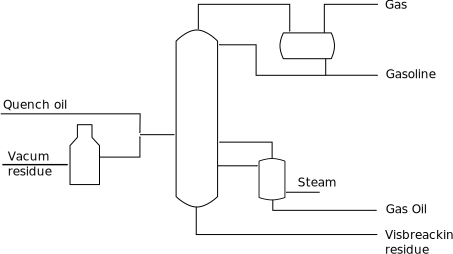
\includegraphics[width=0.80\textwidth]{image/VisbreakingPlant}
	\caption{Schema di un impianto di \textit{visbreaking}}
	\label{fig:Crk:VisbreakingPlant}
\end{figure}


\subsection{Coking}
Il processo di coking permette di ottenere da cariche ad elevato peso molecolare, quali grezzi viscosi derivanti dalla coda del vacuum, nerofumo adatto alla realizzazione di elettrodi. Il processo permette ci� operando ad elevate temperature e con lungi tempi di realizzazione cos� da favorire la dissociazione negli elementi base, come indicato dal diagramma di Francis (\figurename~\ref{fig:Pet:DiagFrancis}). Sempre da questo processo si ottengono benzine ad alto numero di ottano\footnote{D'ora in poi indicato come \textit{NO}.}, ma con elevato contenuto olefinico. Ci� comporta elevata instabilit� del prodotto che pu� essere stabilizzato per idrogenazione.

A causa della formazione di coke all'interno del processo produttivo si hanno notevoli problematiche dovute al deposito di questo all'interno delle condotte, per ovviare a questo problema si sono sviluppati due differenti processi, il \textit{coking ritardato}, dove la carica viene inviata al condotto iniziale ad alta velocit�, in modo da limitare i tempi di contatto e la fase di scissione a dare coke viene rimandata all'uscita ed effettuata all'interno di camere di reazione, e il \textit{fluid coking} dove la scissione avviene in reattore a letto fluidizzato.

\subsubsection{Coking ritardato}
Lo schema dell'impianto � visibile in \figurename~\ref{fig:Crk:CokingPlant}. Il flusso entrante viene inviato ad una colonna che separa le diverse specie entranti sfruttando il calore delle sostanze che hanno gi� subito il cracking. Dal fondo della colonna si ottengono le specie ad alto PM che vengono inviati al forno dove vengono riscaldate fino a una temperatura di circa $550^oC$, e la carica viene poi trasportata velocemente fino alle due camere di reazione (chiamate \textit{coke drums}) dove si ha la vera scissione. Le due coke drums vengono commutate tra fase di riempimento e di svuotamento del coke, evitando cos� l'accumulo all'interno dell'impianto produttivo. La carica, dopo aver sottratto il coke prodotto, viene rinviata alla colonna di rettifica dove si separano, dalla parte superiore, gas e gasoli, mentre dalla parte centrale vengono sottratti i gasoli pesanti.
\begin{figure}[htbp]
	\centering
		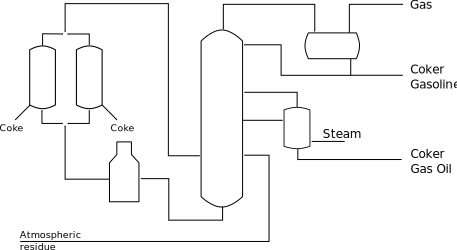
\includegraphics[width=0.80\textwidth]{image/CokingPlant}
	\caption{Schema di un impianto di \textit{coking ritardato}}
	\label{fig:Crk:CokingPlant}
\end{figure}

\subsubsection{Fluid coking}
Un impianto di fluid coking � visibile in \figurename~\ref{fig:Crk:FluidCokingPlant}, ove sono evidenti le strutture principali, quali il reattore di cracking (\textit{R}), la camera di combustione del coke (\textit{B}) e la colonna di rettifica per la separazione delle diverse frazioni petrolifere.

La carica, viene inviata direttamente nel reattore \textit{R} dove viene a contatto con il coke rovente (circa $600^oC$), sottraendo calore a questo subisce crackizzazione e passa allo stato vapore. Il vapore sale nella colonna di rettifica dove viene separato nelle diverse frazioni. La parte che non ha subito cracking o che comunque ha ancora una temperatura di ebollizione troppo elevata torna nella camera di cracking. Il coke che si � prodotto (oltre a quello che era gi� presente nella camera), viene inviato nella camera \textit{B} dove si ha una parziale combustione con aria, permettendo cos� di innalzare la temperatura prima di essere rimandato in \textit{R}.

Una parte del coke che viene inviato in \textit{B} viene sottratto dall'impianto (coke prodotto), mentre i gas di combustione vengono prima inviati in un ciclone (\textit{C}) per eliminare le particelle carboniose che potrebbero essere trascinate; successivamente il calore che essi trasportano viene utilizzato per produrre vapore e infine vengono espulsi dall'impianto.

Il letto in \textit{R} viene mantenuto fluidizzato dai vapori prodotti dalla carica che viene vaporizzata a contatto con il coke.

\begin{figure}[htbp]
	\centering
		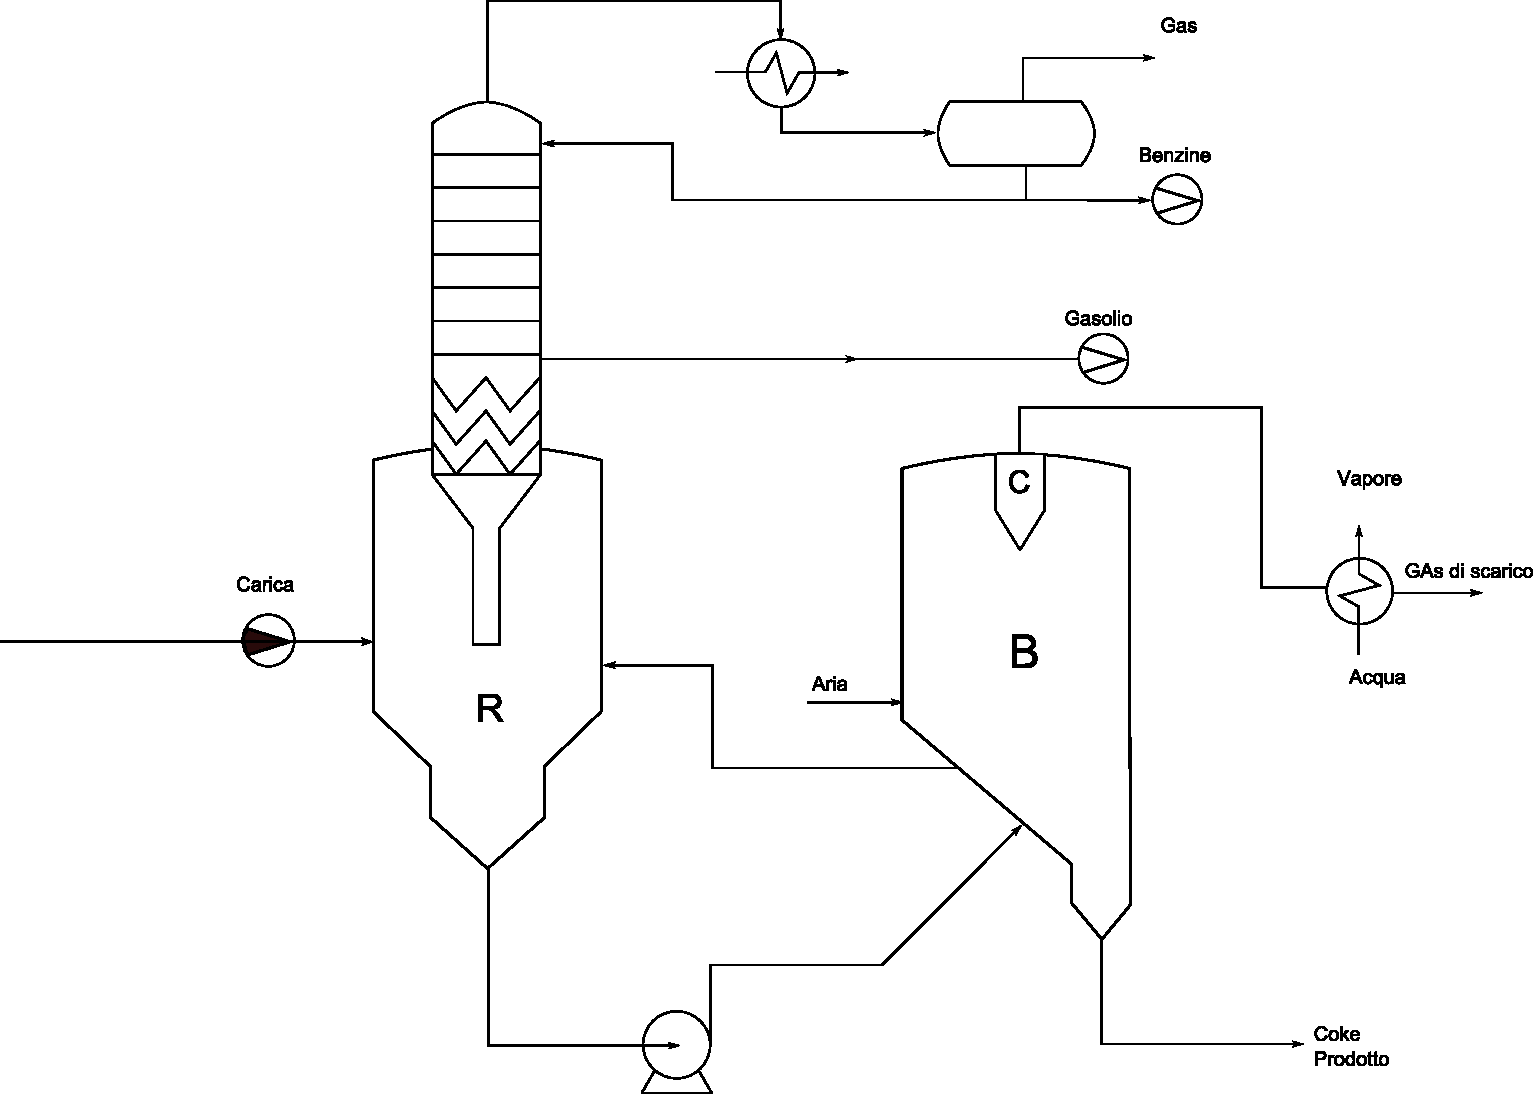
\includegraphics[width=0.95\textwidth]{image/FluidCoking}
	\caption{Schema di un impianto di \textit{fluid coking}}
	\label{fig:Crk:FluidCokingPlant}
\end{figure}

% ========================================================= %
% ========================================================= %
% ========================================================= %
% ========================================================= %
% ========================================================= %
\section{Cracking catalitico}
Il cracking catalitico ha una funzione simile a quella del cracking termico, ma a causa del diverso meccanismo con cui avviene la reazione si ha una diversa distribuzione dei prodotti; in \tablename~\ref{tab:Crk:ConfrontoCTCC} � evidente la differenza di prodotti ottenuti.
\begin{table}[htbp]
	\centering
		\begin{tabular}{lcc} \hline
			Tipo di idrocarburo   & Cracking termico & Cracking Catalitico \\
													  &    (\% volume)   &    (\% volume)      \\ \hline
			Paraffine lineari     & 23.0             &  5.2                \\
			Paraffine ramificate  & 19.8             & 56.8                \\
			Cicloalcani					  & 10.7             &  4.4                \\
			Benzene 							&  1.3             &  0.9                \\
			Olefine lineari				& 15.7             &  5.3                \\
			Olefine ramificate		& 20.6             & 23.9                \\
			Cicloalcheni					&  6.9             &  1.8                \\ \hline
		\end{tabular}
	\caption{Confronto dei prodotti di \textit{Cracking Termico} e \textit{Cracking Catalitico}}
	\label{tab:Crk:ConfrontoCTCC}
\end{table}

\subsection{Il meccanismo}
A differenza del cracking termico dove il meccanismo � di tipo radicalico nel cracking catalitico si ha un meccanismo carbocationico, favorito dalla presenza di acidi di Br\"onsted. Questi forniscono un protone che attacca il doppio legame di un olefina, generando un carbocatione.

La reazione di inizializzazione vede l'acido di Br\"onsted perdere l'idrogenione che si lega al carbonio di un alchene provocando la scissione del doppio legame e la trasposizione della carica sul carbonio vicinale, il tutto come rappresentato di seguito:
\begin{equation}
	\hspace{1cm}
		\vcenter{\hbox{\dimethylenei[a]{}{1==R$_1$;1W==R$_2$;2W==R$_3$;2==R$_4$}}}
	\hspace{1cm} + HA
	\ce{->}
	\hspace{1cm}
		\vcenter{\hbox{\dimethylenei{1==$^+C$}{1==R$_1$;1W==R$_2$;2W==R$_3$;2==R$_4$}}}
	\hspace{1cm} + A^- 
\end{equation}

Un secondo meccanismo di reazione � ottenuto partendo da paraffine, in questo caso � l'acido di Br\"onsted che estrae lo ione idruro dalla paraffina per dare la base coniugata e idrogeno:
\begin{equation}
	\ce{R_3CH + HA -> R_3C^+ + A^- + H_2}
\end{equation}

Il carbocatione contribuisce poi a propagare la reazione secondo uno dei seguenti meccanismi:
\begin{itemize}
	\item Per reazione con altri idrocarburi, per esempio
		\begin{align*}
			\ce{CH_3C^+HCH_3 +} & \ce{CH_3(CH_2)_{14}CH_3 ->} &                      	\\
													& \ce{CH_3CH_2CH_3 + CH_3C^+H(CH_2)_{13}CH_3 } &
		\end{align*}
	\item Rottura in $\beta$ come per il cracking termico
		\begin{equation*}
			\ce{CH_3C^+HCH_2-R -> CH_3CH=CH_2 + R^+}
		\end{equation*}
\end{itemize}

Da notare che l'ordine di stabilit� dei carbocationi � lo stesso dei radicali, ovvero i carbocationi terziari sono pi� stabili dei secondari che a loro volta sono pi� stabili dei primari, la differenza tra i due meccanismi � dato dal tempo di esistenza della specie, infatti per i carbocationi � molto maggiore e quindi sono favorite le trasposizioni verso i carbocationi pi� stabili.

La trasposizione avviene o tramite della migrazione dello ione ioduro nella molecola
\begin{equation}
	\hspace{1cm}
		\vcenter{\hbox{\dimethylenei{1==CH;2==C$^+$}{1==R$_1$;1W==H;2==H;2W==R$_2$}}}
	\hspace{1cm}
	\ce{->}
	\hspace{1cm}
		\vcenter{\hbox{\dimethylenei{1==C$^+$;2==CH}{1==R$_1$;1W==H;2==H;2W==R$_2$}}}
	\hspace{1cm}
\end{equation}
o tramite migrazione alchilica
\begin{equation}
	\hspace{1cm}
		\vcenter{\hbox{\dimethylenei{1==C;2==C$^+$}{1==R$_1$;1W==H;2==H;2W==CH$_3$}}}
	\hspace{1.5cm}
	\ce{->}
	\hspace{0.5cm}
		\vcenter{\hbox{\dimethylenei{1==CH$_3$;2==C$^+$}{2==R$_1$;2W==CH$_3$}}}
	\hspace{1cm}
\end{equation}
ancora pi� stabili sono i carbocationi allilici e benzilici.

Sono favorite le reazioni meno esotermiche, in particolare non si formano i carbocationi $H^+$, $CH_3^+$ e $C_2H_5^+$, ma si hanno principalmente paraffine e olefine $C_3$ - $C_5$. Per gli aromatici la situazione � simile e si ha principalmente formazione di benzene (poco) e toluene (molto), poich� il sostituente $CH_3$ non viene attaccato.

\subsection{I catalizzatori}
I catalizzatori utilizzati negli impianti di crackizzazione devono possedere i seguenti requisiti:
\begin{itemize}
	\item Stabilit� nelle condizioni di reazione, non devono quindi subire modifiche strutturali (sinterizzazione) o perdite causate da sublimazione.
	\item Devono possedere una elevata acidit� per favorire la formazione di carbocationi
	\item Devono possedere una elevata area interfacciale tra reagenti e catalizzatori
\end{itemize}
Tra i catalizzatori che rispecchiano questi requisiti sono stati individuati i silico-alluminati ad elevata area superficiale. Di questi possono essere utilizzati quelli amorfi, in cui si ha una presenza del 10-25\% di $Al_2O_3$, e i cristallini chiamati anche zeoliti\footnote{A volte sono anche chiamati setacci molecolari.}.

Questi ultimi sono i pi� attivi e sono composti da allumino-silicati con molta acqua di cristallizzazione; consentono di avere maggiori rese in benzine a scapito della produzione di idrocarburi leggieri, inoltre formano meno coke e sono meno sensibili ai veleni che tendono a diminuire l'attivit� del catalizzatore.

\subsubsection{I veleni}
Il catalizzatore a base di silico-alluminati (sia amorfi che cristallini), � inibito da alcune sostanze che diminuiscono l'attivit�, in particolare sono particolarmente nocive le sostanze basiche, che si legano ai gruppi acidi presenti sottraendo centri attivi, eccessi di acqua che bagnando la superficie ne riducono l'attivit� e impurezze dei metalli di transizione (in particolare V, As, Fe e Ni). Non � inoltre trascurabile la diminuzione di attivit� provocata dal deposito di coke sulla superficie catalitica.

\subsection{Problematiche}
Come detto precedentemente nel cracking si favorisce anche la deidrogenazione dei composti della carica con la conseguente formazione di sostanze aromatiche e insature. A causa delle condizioni operative si ha anche la condensazione di questi a dare prodotti aromatici ad alto meso molecolare, di conseguenza questi prodotti peciosi, depositandosi sul catalizzatore, ne diminuiscono l'attivit� e pongono la necessit� di processi di rigenerazione per evitarne la sostituzione.

La risoluzione a questo problema � effettuata accoppiandola al processo di riscaldamento, infatti il cracking � un processo endotermico e necessita quindi di elevate quantit� di calore, che pu� essere fornito come calore sensibile del catalizzatore che questo accumula facendo bruciare (a temperature di circa $600-700^oC$) i residui carboniosi che si formano sulla sua superficie. Il rapporto istantaneo tra il catalizzatore e la carica che fluisce su di esso � di circa 10 a 1 in peso e ci� consente un certo equilibrio tra le fasi di cracking e rigenerazione. In questo modo i prodotti di scarto che si otterrebbero (coke e prodotti peciosi) vengono riutilizzati nel processo di combustione per fornire calore al processo.

\subsection{Cracking Catalitico Fluido (\textit{FCC})}
Il cracking catalitico in letto fluido � un impianto in cui il processo di cracking catalitico avviene in un reattore a letto fluido consentendo cos� un processo in continuo che non necessita di una doppia camera di reazione come negli impianti di fluid cocking (\figurename~\ref{fig:Crk:FluidCokingPlant}) che deve essere alternata, ma � sufficiente una sola camera da cui il catalizzatore viene sottratto e reimmesso in maniera continua.

L'utilizzo di questo tipo di impianto porta anche ad un migliore controllo della temperatura e una perdita di catalizzatore molto ridotta grazie alla presenza di cicloni sulla testa.

\subsubsection{Unit� FFC}
Una tipica unit� di FCC � composta oltre dall'apparecchiatura di cracking e di rigenerazione di catalizzatore da tutta una serie di apparati per il corretto funzionamento. Prendiamo in consideriamo l'impianto rappresentato in \figurename~\ref{fig:Crk:FluidCokingPlant}, sono evidenti:
\begin{enumerate}[\hspace{1cm}A:]
	\item Reattore di cracking
	\item Stripper
	\item Rigeneratore
	\item Riser
	\item Condotte di collegamento
	\item Cicloni
	\item Compressore per l'aria
	\item Turbina di espansione per i gas di scarico
	\item Generatore di vapore dai gas esausti
	\item Frazionatore
	\item Assorbitore
	\item Debutanatore
	\item Depropanatore
\end{enumerate}
I tipi di reattore utilizzati possono differire per il posizionamento delle due unit� di cracking e di rigenerazione ma in ogni caso conterranno, oltre a queste due, un apparato di separazione del catalizzatore (dei cicloni, solitamente posizionati in una unit� chiamata \textit{Cyclone vessel}) e un collegamento tra i due dove scorre il catalizzatore che deve essere spostato (\textit{Riser})
\begin{figure}[htbp]
	\centering
		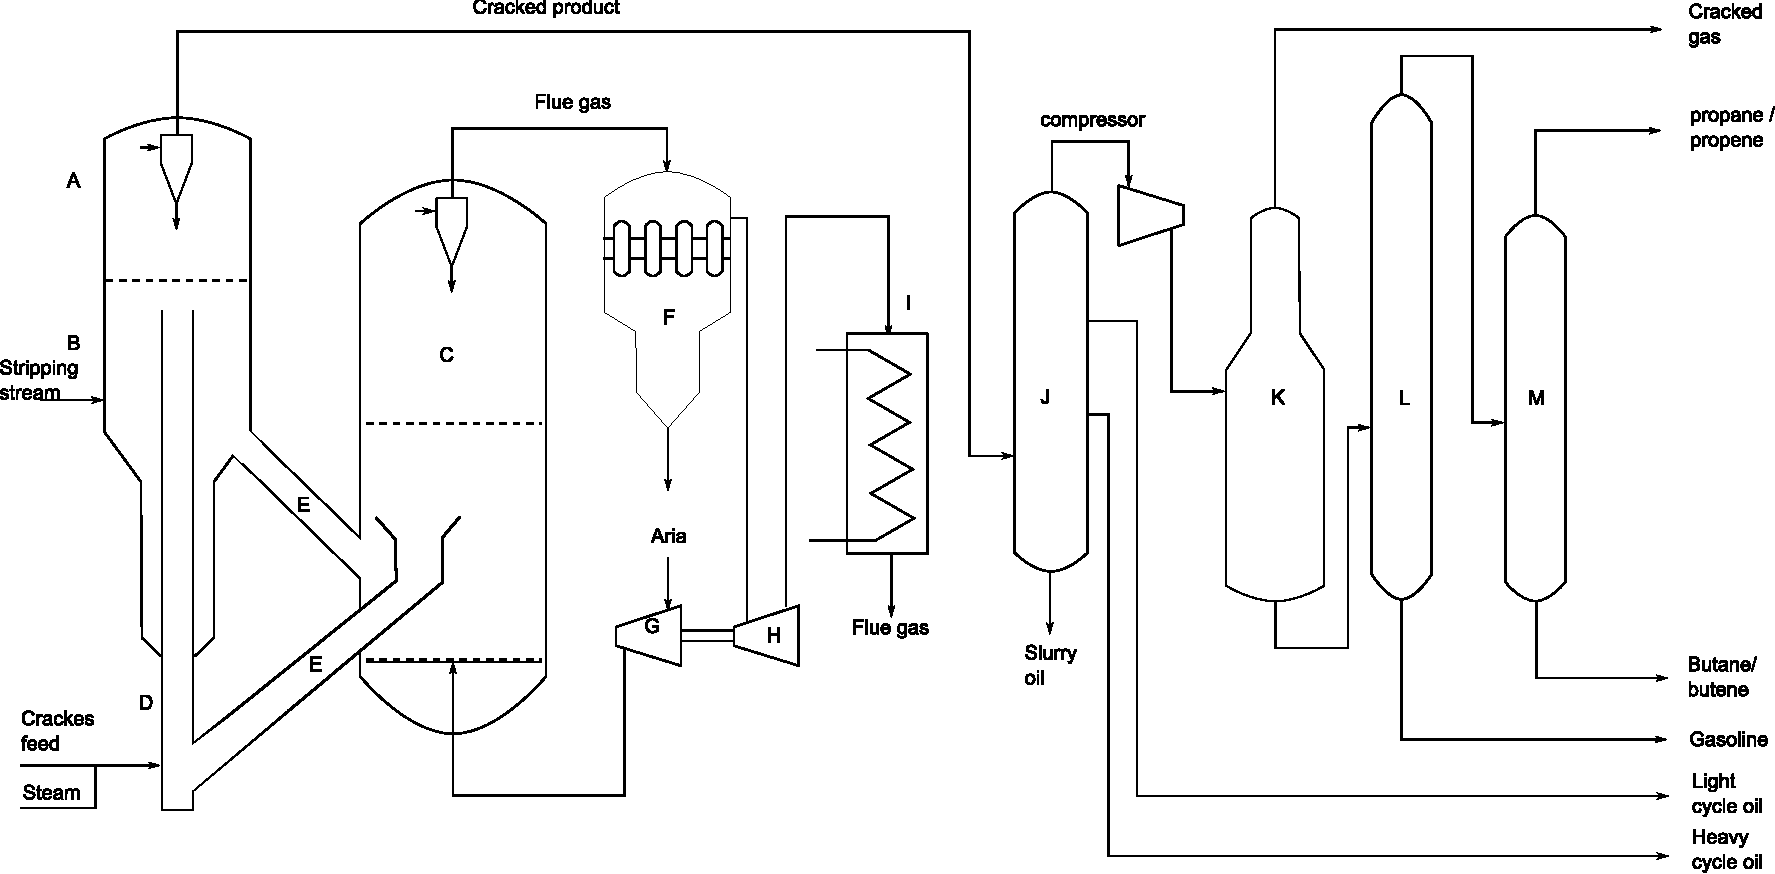
\includegraphics[angle=90,width=0.60\textwidth]{image/FCCPlant.pdf}
	\caption{Impianto FCC}
	\label{fig:crk:FCCPlant}
\end{figure}

\section{Hydrotreating}
I processi catalitici sono destinati a migliorare la qualit� dei prodotti petroliferi mediante idrogenazione sono stati introdotti a seguito di uso di petrolio ad alto tenore di zolfo, alla regolamentazione degli inquinanti e dell'aumento dei prodotti di cracking.

La funzione principale dell'hydrotreting � l'idrodesolforazione (HDS) a \ce{H_2S}, che viene poi separato per estrazione con un solvente (solitamente ammina o miscela di carbonati) e successivamente convertito in zolfo elementare in un impianto \textit{Claus}.

Possono essere utilizzati due diversi tipi di processo, una prima tipologia � studiata per il trattamento di sostanze in fase gassosa (hydrotreating della benzina), mentre una seconda lavora in fase liquida (hydrotreating e desolforazione di medi distillati del gasolio).

I catalizzatori utilizzati in questo processo sono principalmente basati su miscele di \ce{Co}, \ce{Mo} e \ce{Ni}, in \tablename~\ref{tab:Crk:Hydrotreating} sono evidenti le condizioni operative del processo in funzione del tipo di processo\footnote{\textit{GO}: Gas Oil; \textit{VGO}: Vacum Gas Oil; \textit{ARDS}: Atm Residue desulfrization; \textit{HCR}: Hydrocracking. \textit{LHSW} Liquid Hourly Spave Velocity (volume di reagente per volume di catalzzatore)}.

\begin{table}[htbp]
	\centering
		\begin{tabular}{lcccr} \hline
			Processo di 	& Temperature & Pressione 				 	& LHSV		&	Consumo 						\\ 
			Hydrotreating	&	($^oC$)			&	parziale						&					&	di idrogeno 				\\
										& 						&	di \ce{H_2} (atm)		&					& ($Nm^3/m^{3}$) 		\\ \hline
			Naphta				&	320					& 10-20								&	3.0-8.0	& 2-10								\\
			Kerosene			& 330					& 20-30								& 2.0-5.0	& 5-15								\\
			Atm. GO				& 340					& 25-40								& 1.5-4.0	& 20-40								\\
			VGO						& 360					& 50-90								& 1.0-2.0	& 50-80								\\
			ARDS					& 370-410			& 80-130							& 0.2-0.5	& 100-175							\\
			VGO HCR				& 380-410			& 90-140							& 1.0-2.0	& 150-300							\\
			Residuo HCR		& 400-440			& 100-150							& 0.2-0.5	& 150-300							\\ \hline
		\end{tabular}
	\caption{Condizioni tipiche dei diversi processi di hydrotreating}
	\label{tab:Crk:Hydrotreating}
\end{table}

\section{Steam Cracking}
Il processo di steamcking ha lo scopo di trasformare la carica in ingresso in idrocarburi a basso peso molecolare (olefine). La frazione da trattare dipende dal materiale di partenza disponibile; in America, dove si ha elevata disponibilit� di gas naturale viene usata la frazione pesante del GPL come alimentazione, mentre in Europa, dove questa non � sufficiente per soddisfare le esigenze viene utilizzata nafta, anche se con rese inferiori.

\subsubsection{Aspetti termodinamici}
La reazione deidrogenazione di etano:
\begin{equation}
	\ce{C_2H_6 -> C_2H_4 + H_2}
\end{equation}
ha un $\Delta H = 34 Kcal/mol$ da cui � evidente che si tratta di una reazione endotermica e ha un $\Delta G^o = 0$ a circa $800^oC$ (infatti operiamo a circa questa temperatura). La frazione molare dell'etilene all'equilibrio � di 0.333 (a $800^oC$ e per una pressione di circa 3 atm).

La resa potrebbe essere innalzata in diversi modi, ovvero aumentando la temperatura del processo, nel qual caso migliorerebbe anche al cinetica del processo, abbassando al pressione operativa (operazione che viene gi� effettuata diluendo con vapore) e riducendo i tempi di contatto e di conseguenza diminuendo al decomposizione a coke e idrogeno.

\subsubsection{Le condizioni operative}
Il processo opera ad una temperatura di $700-800^oC$ e con tempi di permanenza molto ridotti (1 secondo circa) per evitare la reazione ulteriore delle olefine prodotte. La pressione operativa � limitata il pi� possibile poich� una pressione bassa favorisce la formazione di olelfine a basso PM, ma al contempo deve essere limitata la possibilit� di formazione di coke e benzene.

Poich� � antieconomico lavorare in depressione si opta per l'utilizzo di vapore come diluente in modo che la pressione parziale degli idrocarburi sia subatmosferica, inoltre l'utilizzo di vapore porta anche ad alcuni vantaggi; innananzitutto inibisce al formazione di composti carboniosi che vengono trasformati in idrogeno, \ce{CO} e \ce{CO_2} e soprattutto apporta parte del calore sensibile necessario alla reazione. Il rapporto tra il quantitativo di vapore e di idrocarburi inviati va da $0.4/1$ a $1/1$ in peso (all'incirca 1 a 6 in volume).

Da notare anche che non � possibile abbassare troppo la pressione operativa poich� devono comunque essere superate le perdite di carico della condotta presente nel forno di riscaldamento e reazione.

\subsubsection{L'impianto}
L'impianto � composto da un miscelatore dei flussi di vapore e idrocarburi, che poi vengono immessi in un forno di riscaldamento composto da una serie di tubi di nichel-cromo con lunghezze che vanno dai 50 ai 200m e con diametri di $80-120mm$. La scelta del materiale produttivo delle tubazioni � data dalla resistenza che questo deve mantenere alle temperature operative ($T_{max} = 1050^oC$).

Sempre per il motivo accennato precedentemente, ovvero la possibilit� di insorgere di reazioni secondarie delle olefine se i tempi di reazione risultano elevati, � necessario procedere ad un rapido abbassamento della temperatura all'uscita della camera di reazione (operazione chiamata di \textit{quench}). Questo viene fatto, prima, inviando acqua alla camicia esterna delle condotte in modo da recuperare il calore per la produzione di vapore ($T_{out} \approx 200^oC$), mentre successivamente la temperatura viene ulteriormente abbassata per mezzo di olio.

A seguito del raffreddamento viene effettuata una serie di separazioni per eliminare l'acqua e il vapore presente dalla frazione idrocarburica e successivamente per eliminare i gas idrocarburici dall'acqua residua.

L'ultimo passaggio prevede la disidratazione per evitare la formazione di ghiaccio nelle fasi successive del processo di separazione e un lavaggio con soda caustica per l'eliminazione di \ce{H_2S} e \ce{CO_2}.

\subsubsection{Problematiche}
Tra i problemi principali che insorgono degli impianti di Steam Cracking vi sono la formazione di depositi di coke all'interno delle condotte che portano ad una diminuzione della sezione di passaggio e di conseguenza l'aumento delle perdite di carico. Altro problema portato dal deposito all'interno delle tubazioni � la diminuzione della conducibilit� termica dal forno all'interno delle condotte con conseguenti problemi di riscaldamento del fluido e conseguente perdita della resa verso i prodotti desiderati.

Per risolvere alcuni di questi problemi e ottimizzare lo scambio termico dall'esterno verso l'interno sono stati studiate e applicate diverse tecniche costruttive differenti. Inizialmente le tubature erano disposte orizzontalmente nella camera di riscaldamento, ma ci� portava ad alte perdite di carico e alti tempi di resistenza, nonch� lunghezze superiori alle centinaia di metri (\figurename~\ref{fig:Crk:SerpPirolisi:Orizzontali}).
Successivamente si � passati ad una disposizione dei tubi verticale (\figurename~\ref{fig:Crk:SerpPirolisi:Verticali}), ci� comportava ad una diminuzione della lunghezza (circa $70-90m$), ma fu soprattutto la messa in posa di tubi ellittici in modo da ottimizzare lo scambio termico con l'esterno a portare notevoli miglioramenti (tecnologia \textit{Mitsubushi}).
Un ulteriore vantaggio fu introdotto con la scelta di condotte a diametro variabile (\figurename~\ref{fig:Crk:SerpPirolisi:DiamVariab}) in cui il diametro aumentava in funzione della lunghezza del percorso dalla fase di immissione (\textit{Swaged - Tapered}) o dall'utilizzo della alimentazioni intermedie (\textit{ESSO}).
Infine vennero inserite una serie di condotte in cui l'alimentazione viene immessa in diverse condotte che man mano si uniscono per fuoriuscire da un unico tubo con diametro maggiore rispetto a quelli iniziali (\figurename~\ref{fig:Crk:SerpPirolisi:SplitCoil}).
\begin{figure}[htbp]
	\centering
		\subfigure[Serpentini orizzontali]{
			\label{fig:Crk:SerpPirolisi:Orizzontali}
			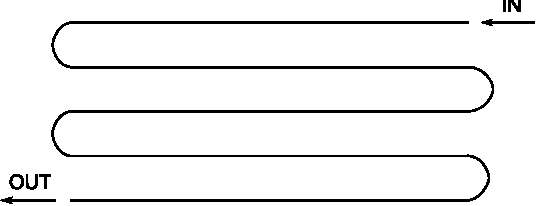
\includegraphics[width=0.45\textwidth]{image/SerpentiniPirolisiOrizzontali}
		}
		\subfigure[Serpentini verticali]{
			\label{fig:Crk:SerpPirolisi:Verticali}
			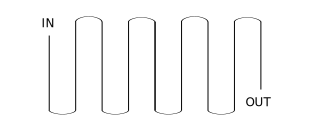
\includegraphics[width=0.45\textwidth]{image/SerpentiniPirolisiVerticali}
		}
		\subfigure[Serpentini a diametro variabile]{
			\label{fig:Crk:SerpPirolisi:DiamVariab}
			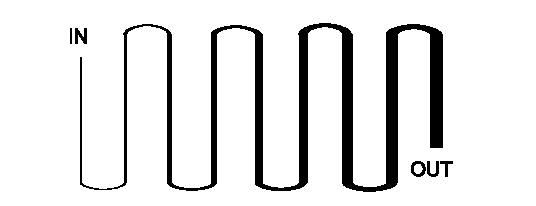
\includegraphics[width=0.45\textwidth]{image/SerpentiniPirolisiDiamVariabile}
		}
		\subfigure[Serpentini \textit{split coil}]{
			\label{fig:Crk:SerpPirolisi:SplitCoil}
			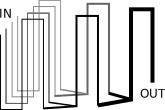
\includegraphics[width=0.45\textwidth]{image/SerpentiniPirolisiSplitCoil}
		}
	\caption{Serpentini di pirolisi}
	\label{fig:Crk:SerpPirolisi}
\end{figure}

	 \chapter{Il reforming}
Con reforming intendiamo tutta quella serie di processi atti a migliorare le caratteristiche dei prodotti petroliferi tramite modificazione della struttura dei composti, in particolare si parte da benzine di prima distillazione (costituite da nafteni, cicloesani e paraffine lineari) per arrivare a benzine con N.O.\footnote{Ricordiamo che con il termine N.O. indichiamo il numero di ottano della benzina.} maggiori.
Altri prodotti desiderati sono strutture aromatiche, precursici di molti prodotti dell'industria petrolchimica, e idrogeno.

L'intero processo si basa su reazioni che trasformano paraffine lineari e nafteni in paraffine ramificate e aromatici (per esempio da cicloesano a benzene o \textit{n}-ottano in 2,2,3-trimetilpentano). Le reazioni principali che avvengono sono le \textit{deidrogenazioni ad aromatici}, l'\textit{isomerizzazione di paraffine lineari}, \textit{hydrocracking di paraffine} e le \textit{deidrociclizzazione di paraffine}.

Inizialmente (anni '30 e '40) il processo veniva compiuto per via termica, ovvero si operava a temperature di circa $580^oC$ e inserendo la carica questa veniva modificata senza necessitare di nessun catalizzatore; ci�, per�, portava a notevoli perdite di materia a causa di deidrogenazioni e reazioni indesiderate, per di pi� non consentiva di raggiungere N.O. superiori a 80. Per questi motivi attualmente si utilizza esclusivamente il reforming catalitico.

\section{Il reforming catalitico}
Come indicato precedentemente lo scopo del reforming catalitico � quello di migliorare le prestazioni delle benzine limitando le perdite dei reagenti iniziali e limitando le condizioni operative.

\subsection{Le reazioni}
Poich� il processo di reforming coinvolge una serie vasta di reazioni queste sono state raggruppate in alcune classi significative che ora andremo ad analizzare singolarmente.
\subsubsection{Deidrogenazioni}
Le deidrogenazioni sono reazioni endotermiche che quindi necessitano calore per avvenire, come evidente dal diagramma di Francis sono favorite dalle alte temperature ed in particolare possono essere considerate deidrogenazioni di alcani per dare alcheni:
\begin{equation}
	\vcenter{\hbox{\heptamethylene{}{}}}
	\rightarrow
	\vcenter{\hbox{\heptamethylene[e]{}{}}} + H_2
\end{equation}
da cicloalcani per dare aromatici:
\begin{equation}
	\vcenter{\hbox{\cyclohexanev{}{}}}
	\rightarrow
	\vcenter{\hbox{\cyclohexanev[A]{}{}}} + 3 H_2
\end{equation}
da cicloalcheni per dare aromatici:
\begin{equation}
	\vcenter{\hbox{\cyclohexanev[a]{}{}}}
	\rightarrow
	\vcenter{\hbox{\cyclohexanev[A]{}{}}} + 2 H_2
\end{equation}

\subsubsection{Deidroisomerizzazioni}
I questo caso un anello a paraffinico modifica la sua struttura e viene deidrogenato per dare un prodotto aromatico:
\begin{equation}
	\vcenter{\hbox{\fiveheterovi{}{1==$CH_3$}}}
	\rightarrow
	\vcenter{\hbox{\cyclohexanev{}{}}}
	\rightarrow
	\vcenter{\hbox{\cyclohexanev[A]{}{}}} + 3 H_2
\end{equation}

\subsubsection{Deidrociclizzazioni}
In questo caso una paraffina lineare subisce ciclizzazione per poi subire una aromatizzazione
\begin{equation}
	\vcenter{\hbox{\heptamethylene{}{}}}
	\rightarrow
	\vcenter{\hbox{\sixheterov{}{1==$CH_3$}}} + H_2
	\rightarrow
	\vcenter{\hbox{\sixheterov[A]{}{1==$CH_3$}}} + 4 H_2
\end{equation}
oppure si pu� partire da una olefina per avere chiusura ad anello e successiva aromatizzazione
\begin{equation}
	\vcenter{\hbox{\heptamethylene[d]{}{}}}
	\rightarrow
	\vcenter{\hbox{\sixheterov{}{1==$CH_3$}}}
	\rightarrow
	\vcenter{\hbox{\sixheterov[A]{}{1==$CH_3$}}} + 4 H_2
\end{equation}

\subsubsection{Isomerizzazioni}
Le isomerizzazioni portano a trasposizioni di alcuni gruppi per dare paraffine, olefine o aromatici con struttura modificata, per esempio, per paraffine:
\begin{equation}
	\vcenter{\hbox{\heptamethylene{}{}}}
	\rightarrow
	\vcenter{\hbox{\hexamethylene{}{2==$CH_3$}}}
\end{equation}
per cicloalcani:
\begin{equation}
	\vcenter{\hbox{\fiveheterovi{}{1==$CH_3$}}}
	\rightarrow
	\vcenter{\hbox{\cyclohexanev{}{}}}
\end{equation}
mentre per alchilaromatici:
\begin{equation}
	\vcenter{\hbox{\sixheterov[A]{}{1==$CH_3$;4==$CH_3$}}}
	\rightarrow
	\vcenter{\hbox{\sixheterov[A]{}{1==$CH_3$;3==$CH_3$}}}
\end{equation}

\subsubsection{Idroisomerizzazioni}
In questo caso le olefine vengono idrogenate a paraffine subendo anche trasposizione e dando quindi paraffine ramificate:
\begin{equation}
	\vcenter{\hbox{\heptamethylene[e]{}{}}} + H_2
	\rightarrow
	\vcenter{\hbox{\hexamethylene{}{2==$CH_3$}}} 	
\end{equation}

\subsubsection{Idrodealchilazioni}
In questo caso i composti aromatici sostituiti subiscono eliminazione del sostituente per dare aromatici non sostituiti pi� paraffine:
\begin{equation}
	\vcenter{\hbox{\sixheterov[A]{}{1==$CH_3$;}}} + H_2
	\rightarrow
	\vcenter{\hbox{\sixheterov[A]{}{}}} + CH_4
\end{equation}

\subsubsection{Hydrocreacking}
La paraffina di partenza � separate in due paraffine distinte:
\begin{equation}
	\ce{CH_3(CH_2)_8CH_3} + H_2
	\rightarrow
	\vcenter{\hbox{\tetramethylene{}{}}} + \vcenter{\hbox{\hexamethylene{}{}}}
\end{equation}
\begin{equation}
	\vcenter{\hbox{\tetramethylene{4==R}{2==$CH_3$}}}
	\rightarrow
	\vcenter{\hbox{\tetramethylene{4==R}{}}} + CH_4
\end{equation}

\subsubsection{Idrodesolforazioni}
Viene eliminato lo zolfo interno ai composti organici, che deve essere successivamente eliminato per evitare l'avvelenamento dei catalizzatori:
\begin{equation}
	\vcenter{\hbox{\fiveheterovi[bd]{1==S}{}}} + 4H_2
	\rightarrow
	\vcenter{\hbox{\tetramethylene{}{}}} + H_2S
\end{equation}

\subsubsection{Eliminazioni di composti azotati}
Come per la reazione di eliminazione di zolfo si pu� avere eliminazione, dai composti azotati, di ammoniaca:
\begin{equation}
	\vcenter{\hbox{\fiveheterovi[bd]{1==N}{1==H}}} + 4H_2
	\rightarrow
	\vcenter{\hbox{\tetramethylene{}{}}} + NH_3
\end{equation}

\subsubsection{Eliminazione di composti ossigenati}
\begin{equation}
	\vcenter{\hbox{\sixheterovi[A]{}{4==OH}}} + H_2
	\rightarrow
	\vcenter{\hbox{\sixheterovi[A]{}{}}} + H_2O
\end{equation}

\subsection{Il catalizzatore}
Come evidente le reazioni che devono avvenire nella fase di reforming sono principalmente idrogenazioni/deidrogenazioni e trasposizioni, di conseguenza si dovranno utilizzare catalizzatori tali da favorire questi passaggi. Per i primi si utilizza un catalizzatore basato su metallo nobile (tipicamente \ce{Pt}) mentre per le trasposizioni si utilizza un catalizzatore acido.

Dalle informazioni ricavate si � optato per la scelta di un catalizzatore di \ce{Pt-Al_2O_3} eventualmente con la presenza di \ce{Re} per limitare la disattivazione del catalizzatore da parte dei veleni, cio� composti solforati anche con concentrazioni inferiori a 1ppm, composti azotati e clorurati, \ce{As}, \ce{Pb} e \ce{Cu}.

Problemi di disattivazione del catalizzatore portavano alla necessita di fermata dell'impianto per procedere alla rigenerazione tramite ossidazione con aria diluita in azoto (circa il 2\% di ossigeno) per eliminare tutti i depositi carboniosi e una successiva fase di ossiclorurazione per ripristinare la funzionalit� acida del catalizzatore.

\subsection{Le condizioni operative}
Consideriamo, per esempio, la sequenza:
\begin{equation}
	\vcenter{\hbox{\fiveheterovi[]{}{1==$CH_3$}}}
	\rightarrow
	\vcenter{\hbox{\sixheterovi{}{}}}
	\rightarrow
	\vcenter{\hbox{\sixheterovi[A]{}{}}} + 3 H_2
\end{equation}
inizialmente si ha una isomerizzazione, reazione poco favorita termodinamicamente, ma data l'elevata velocit� della successiva deidrogenazione la concentrazione dei prodotti � molto bassa, di conseguenza l'equilibrio viene spostato.

La deidrogenazione successiva da cicloesano a benzene � favorita ad una pressione inferiore rispetto la deidrogenazione da paraffina a olefina e quindi sar� il prodotto pi� facilmente ottenibile. La formazione di prodotti peciosi � limitata dall'operare in presenza di idrogeno, che per�, di contro, sfavorisce anche la produzione di aromatici. 

Un fattore limitante della temperatura � la possibilit� di avere cracking della carica (soprattutto nella fase di preriscaldamento, dove si hanno le temperature maggiori), di conseguenza non si opera a temperature troppo elevate.

Una bassa velocit� spaziale favorisce la reazione di idrocracking, quindi � preferibile evitarle, in pratica le condizioni operative del processo sono scelte in modo che i prodotti siano il pi� possibili conformi alle specifiche richieste, in particolare si opera con processi ad alta pressione (HP) in un range di 30-50bar, per i processi a bassa pressione a 8-20bar. La temperatura operativa si trova nel range compreso tra i $460-530^oC$, la velocit� spaziale (LHSV) � mantenuta ad un valore compreso tra 1 e $5h^{-1}$, mentre il rapporto tra idrogeno e idrocarburi si trova compreso tra 3 e 10 con un valore usuale di 8 (v/v).

\subsection{Il processo}
Inizialmente il processo era stato studiato per essere effettuato in tre reattori a letto fisso in serie a monte dei quali si trovava un sistema di separazione per definire il taglio da trattare. Ogni reattore aveva al suo interno un profilo termico decrescente (il processo � complessivamente endotermico), di conseguenza i vari reattori erano intervallati da dei forni per innalzare la temperatura della carica. La disattivazione del catalizzatore, per�, portava alla necessit� di fermate dell'impianto per la sua sostituzione ogni 6-12 mesi per qualche giorno. Un tipico impianto di questo tipo � visibile in \figurename~\ref{fig:Ref:Plant:StaticBed}.

Una importante innovazione fu introdotta con l'utilizzo dello \textit{swing reactor}, ovvero un sistema che permetteva di avere tre reattori sempre funzionanti mentre un quarto era usato per la rigenerazione, in pratica dei quattro reattori attivi tre erano in fase produttiva, mentre un quarto era in fase rigenerativa, ci� port� a non avere pi� impianti che dovevano essere fermati, ma che potevano operare sempre in continuo e in condizioni pi� spinte. Il prezzo da pagare per questo era l'aumento della complessita realizzativa e di gestione dell'impianto.

Altra importante innovazione inserita � l'utilizzo di reattori a letto fluido, in questo modo il catalizzatore percorre i tre reattori e fuoriuscendo dall'ultimo viene inviato ad una camera di rigenerazione, quindi il catalizzatore viene rigenerato in continuo, permettendo di ottenere risultati ancora migliori nella resa per passaggio della carica e un prolungamento della vita del catalizzatore stesso. Un impianto di questo tipo � visibile in \figurename~\ref{fig:Ref:Plant:FluidBed}
\begin{figure}[htbp]
	\centering
		\subfigure[Con reattori a letto fisso]{
			\label{fig:Ref:Plant:StaticBed}
			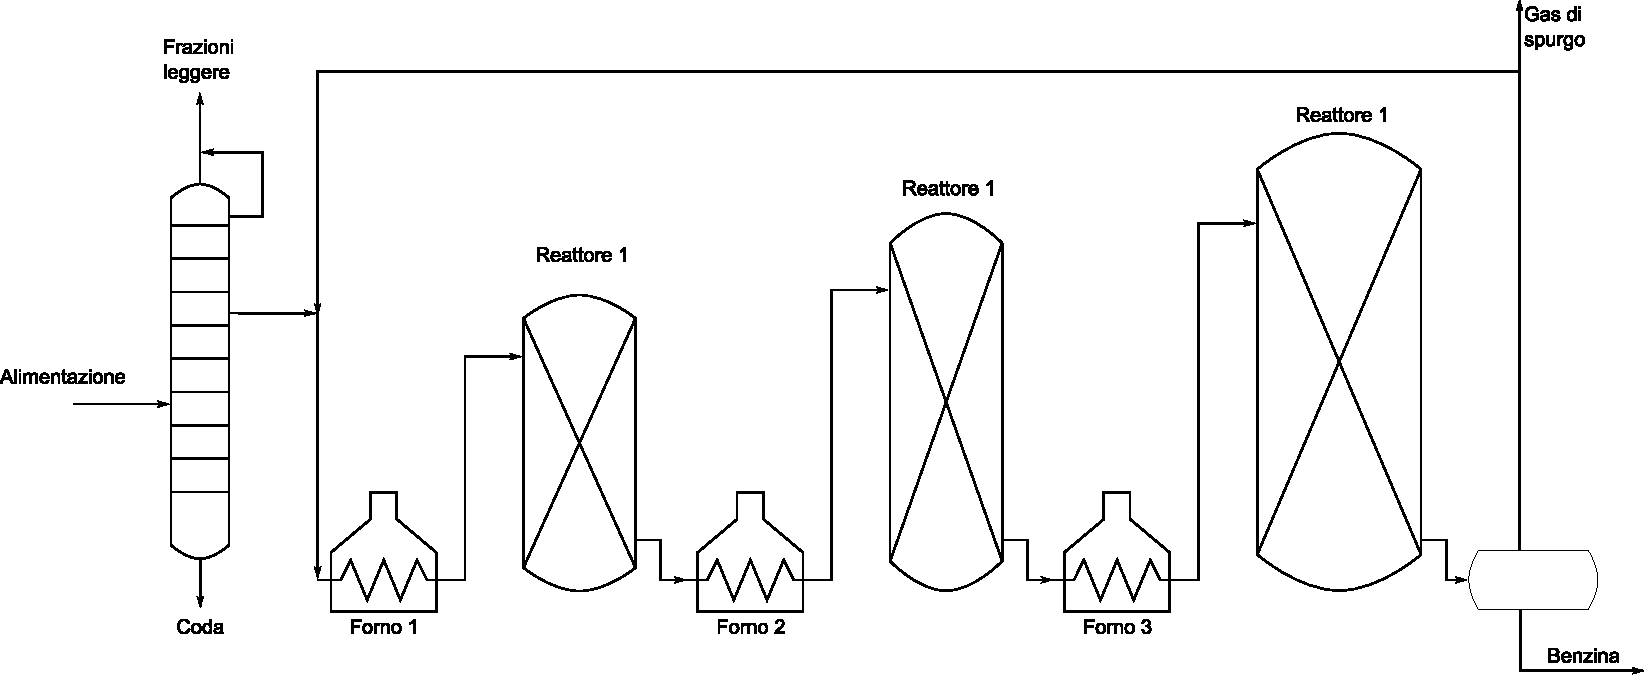
\includegraphics[width=0.85\textwidth]{image/ReformingPlantStaticBed}
		}
		\subfigure[Con reattori a letto fluidizzato]{
			\label{fig:Ref:Plant:FluidBed}
			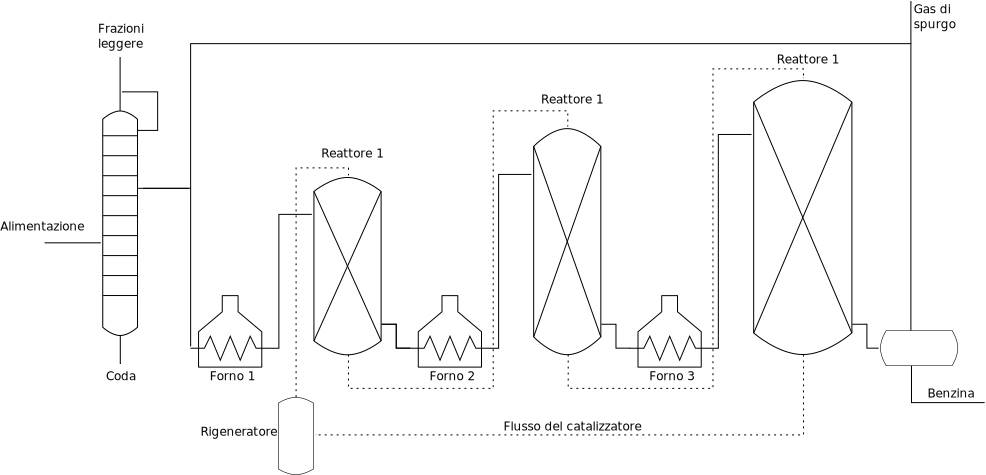
\includegraphics[width=0.85\textwidth]{image/ReformingPlantFluidBed}
		}
	\caption{Tipologie di impianti utilizzati per il cracking catalitico}
	\label{fig:Ref:Plant}
\end{figure}

\subsubsection{I reattori}
I reattori utilizzati sono reattori adiabatici di dimensioni crescenti; la dimensione dei reattori sono in funzione delle temperature raggiunte, infatti nel primo reattore si ha una pi� drastica riduzione della temperatura (il catalizzatore � attivo solo al di sopra di una certa temperatura critica), e quindi il tempo di contatto viene ridotto; la necessit� di avere dimensioni maggiori nei reattori successivi sono date anche dal fatto che le reazioni di deidrogenazioni (le pi� veloci ed endotermiche) avvengono nel primo reattore e per far progredire le reazioni pi� lente negli altri reattori sono necessari tempi di contatto maggiori.

Inizialmente costituiti da reattori a letto fisso a flusso assiale (\figurename~\ref{fig:Ref:Reattori:Assiale}), ci� per� portava a problematiche di rigenerazione del catalizzatore e difficile controllo delle temperature. Vennero di seguito sostituiti da reattori a flusso radiale (\figurename~\ref{fig:Ref:Reattori:Radiale}) che permettono un maggiore controllo termico e successivamente da reattori a letto fluido cosicch� il catalizzatore viene estratto e rigenerato in continuo.
\begin{figure}[htbp]
	\centering
		\subfigure[Flusso assiale]{
			\label{fig:Ref:Reattori:Assiale}
			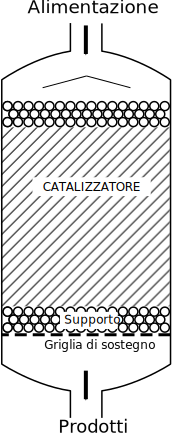
\includegraphics[width=0.25\textwidth]{image/ReattoreFlussoAssaile}
		}\quad\quad\quad\quad
		\subfigure[Flusso radiale]{
			\label{fig:Ref:Reattori:Radiale}
			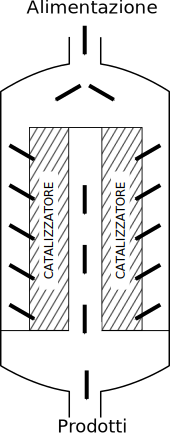
\includegraphics[width=0.25\textwidth]{image/ReattoreFlussoRadiale}
		}
	\caption{Tipologie di reattori utilizzati}
	\label{fig:Ref:Reattori}
\end{figure}

\subsubsection{La rigenerazione del catalizzatore}
Il catalizzatore utilizzato subisce disattivazione da parte di composti azotati e solforati, nonche dai metalli presenti che possono formare leghe con esso, infine il depositarsi di coke sulla superficie, per quanto limitato dall'elevata pressione parziale dell'idrogeno non pu� essere completamente evitato, quindi si ha riduzione della superficie attiva.

La rigenerazione del catalizzatore viene effettuata inizialmente procedendo ad una combustione con aria diluita da azoto per eliminare i residui carboniosi; si opera con una miscela povera di ossigeno, circa al 1-2\% e con temperature di circa $500^oC$.

La riattivazione della funzionalit� acida viene compiuta tramite un processo di ossiclorurazione che ha anche lo scopo di ridisperdere il platino presente all'interno; questa viene compiuta usando \ce{HCl} o una altra specie clorurante, vapore e ossigeno (circa al 10\%).

Nel caso in cui la funzionalit� di idrogenasi sia troppo elevata si pu� ricorrere ad un processo chiamato di \textit{tremperating} in cui si tratta il catalizzatore con una miscela di gas contenenti \ce{H_2S} ad una concentrazione di circa 100ppm.

Il catalizzatore di cracking catalitico pu� cos� essere rigenerato parecchie volte ed ha una vita utile di alcuni anni. Una volta sostituito il catalizzatore si procede ad un recupero di metalli preziosi presenti in esso (principalmente \ce{Pt} ma recentemente anche \ce{Re}).
	 \chapter{Separazione dei BTX}
La miscela dei BTX\footnote{Con \textit{BTX} viene intesa la miscela di aromatici a basso peso molecolare, quindi benzene, toluene, xileni e etilbenzene.} viene facilmente separata inizialmente tramite una rettifica in tre frazioni, rispettivamente composte da benzene ($T_{eb}=80^oC$ circa 60 piatti), toluene ($T_{eb}=110.6^oC$ circa 60 piatti) e xileni e etilbenzene ($T_{eb}=136.2 - 144.4^oC$).

\section{Separazione degli aromatici dagli altri idrocarburi}
Dato il basso range di temperature in cui si trovano tutte le specie che confluiscono nell'impianto di separazione (posizionato subito dopo l'impianto di reforming, che produce una elevata quantit� di aromatici), non � possibile operare con una semplice rettifica anche per l'elevato numero di azeotropi che si formano. si opera, quindi, sfruttando la maggiore polarizzabilit� dei composti aromatici rispetto ai composti paraffinici, si usa quindi un solvente che abbia le seguenti caratteristiche:
\begin{itemize}
	\item Sciolga facilmente e bene i composti aromatici
	\item Non sia completamente miscibile con la frazione idrocarburica
	\item Sia facilmente separabile dal prodotto (per esempio per distillazione)
\end{itemize}
come solventi sono stati scelti, per le loro caratteristiche quelli riportati in \tablename~\ref{tab:btx:solventiEstrazione}
\begin{table}[htbp]
	\centering
		\begin{tabular}{p{5cm}cc} \hline
			Sostanza									&		B.P.		&		Densit�	\\
																&	$T [^oC]$	&		$Kg/L$	\\ \hline
			Glicole dietilenico				& 245 			& 1.05 \\
			\hbox{\pentamethylene{3==O}{1W==OH;5W==OH}} & & \\
			Dimetilsolfossido 				& 190 			& 1.21 \\
			\hbox{\dimethylenei[a]{1==S;2==O}{1==$CH_3$;1W==$CH_3$}} & & \\
			Sulfolano  								& 286 			& 1.26 \\
			\hbox{\fiveheterovi{1==S}{1Sa==O;1Sb==O}} & & \\
			n-formilmorfolina	 				& 2.43 			& 1.15 \\ 
			\hbox{\sixheterovi{1==N;4==O}{1==CHO}} & & \\ \hline
		\end{tabular}
	\caption{Solventi utilizzati per la separazione dei BTX}
	\label{tab:btx:solventiEstrazione}
\end{table}
Uno schema semplificato e abbastanza generico � visibile in \figurename~\ref{fig:btx:extractionPlant}, dove si vede il posizionamento dell'impianto di estrazione degli aromatici all'interno di un impianto di raffineria. I differenti processi utilizzati si basano sull'uso di solventi differenti e le diverse tecniche di separazione dei prodotti.
\begin{figure}[htbp]
	\centering
		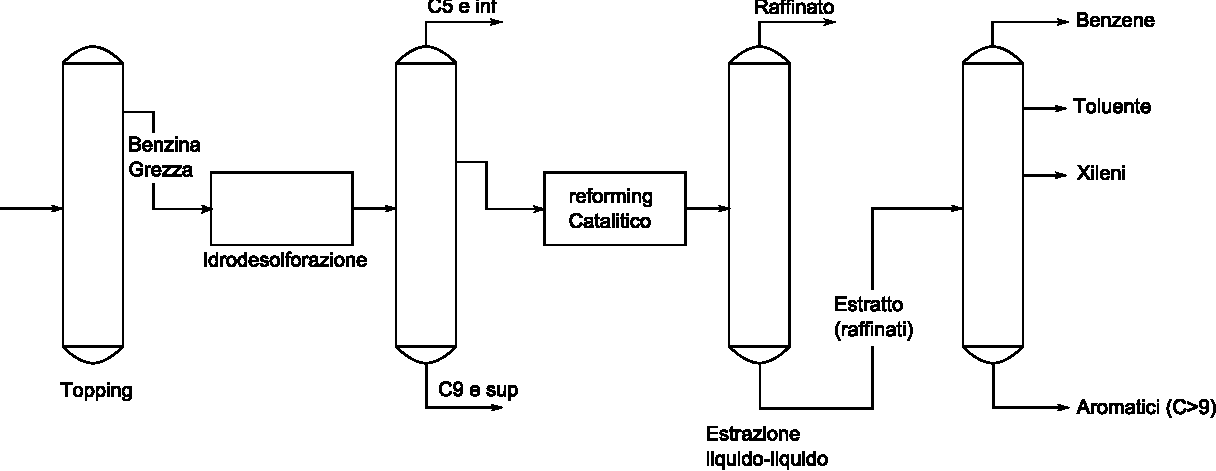
\includegraphics[width=0.80\textwidth]{image/ImpiantoEstrazioneBTX}
	\caption{Rappresentazione della posizione dell'impianto di estrazione di BTX in una raffineria}
	\label{fig:btx:extractionPlant}
\end{figure}

\subsection{Processo UDEX}
\'E il primo processo utilizzato per l'estrazione dei BTX dalla frazione idrocarburica; in questo caso il solvente e l'idrocarburo viaggiano in controcorrente, pertanto per migliorare la prestazioni nella parte finale della colonna viene effettuato un riflusso degli aromatici.

Come solvente viene utilizzato glicole dietilenico con l'aggiunta di acqua per migliorarne ulteriormente le caratteristiche di immiscibilit�; questa non potrebbe essere utilizzata da sola, sia a causa della temperatura di ebollizione che dalla bassa solubilit� con composti aromatici. La temperatura operativa � di circa $175^oC$, mentre la pressione � mantenuta a circa 8bar.

Lo schema dell'impianto � visibile in \figurename~\ref{fig:btx:UDEXPlant}, dove sono evidenti le apparecchiature principali e i flussi, l'alimentazione viene inviata, come gi� detto, in controcorrente con il solvente (DEG miscelato ad acqua), all'uscita dall'estrattore si hanno, come frazione leggera il raffinato composto dall'alimentazione a cui sono stati sottratti gli aromatici, mentre dalla coda esce il solvente contenete gli aromatici. Questo viene inviato allo stripper che opera alla stessa temperatura, ma a pressione inferiore effettuando quindi una distillazione flash. Dalla testa usciranno i composti aromatici e l'acqua mentre dalla coda il solvente che viene rinviato all'estrattore. La miscela acqua/aromatici viene fatta condensare (tramite abbassamento delle temperature) e successivamente inviata ad uno smiscelatore, da cui vengono allontanati i composti aromatici che in parte vengono inviati come riflusso all'estrattore, e in parte sottratti come prodotto. l'acqua uscente dal separatore viene riciclata.
\begin{figure}[htbp]
	\centering
		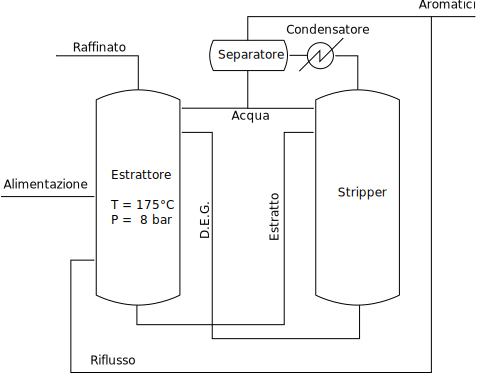
\includegraphics[width=0.60\textwidth]{image/ImpiantoUDEX}
	\caption{Rappresentazione dell'impianto UDEX}
	\label{fig:btx:UDEXPlant}
\end{figure}

Gli impianti sviluppati successivamente sono tutti perfezionamenti di questa tipologia di impianto.

\subsection{Processo SNAM-Progetti}
L'impianto realizzato dalla SNAM-Progetti ricalca lo schema dell'impianto BTX ma utilizza dimetilformalina come solvente e introduce altre due apparecchiature per il recupero del solvente presente nel raffinato e uno stripper iniziale per spingere la selettivit� rimandando all'estrattore le paraffine. Lo schema di processo � visibile in \figurename~\ref{fig:btx:SNAMPlant}, dove sono ben evidenti gli elementi principali dell'impianto.

La carica iniziale viene inviata ad un estrattore in cui il solvente (dimetilformalina) procede controcorrente, dalla testa esce la carica idrocarburica che viene mandata ad una seconda colonna di estrazione, in questo caso il solvente � costituito da acqua che asporta anche le ultime traccie di dimetilformalina dalla miscela idrocarburica.

Il solvente contenente gli aromatici viene dapprima inviato ad uno stripper che elimina le tracce di idrocarburi presenti e le reinvia all'estrattore primario, mentre il solvente contenete i BTX viene inviato ad una seconda colonna di stripping per la separazione dei BTX (e acqua) dal solvente; questo viene rinviato alla colonna di estrazione, mentre i BTX e l'acqua subiscono smiscelazione e separazione, ma mentre i BTX vengono eliminati dal processo (sono il prodotto desiderato), l'acqua prima di ritornare nell'estrattore confluisce (in parte) nella colonna di lavaggio del raffinato vista inizialmente per recuperare il solvente.
\begin{figure}[htbp]
	\centering
		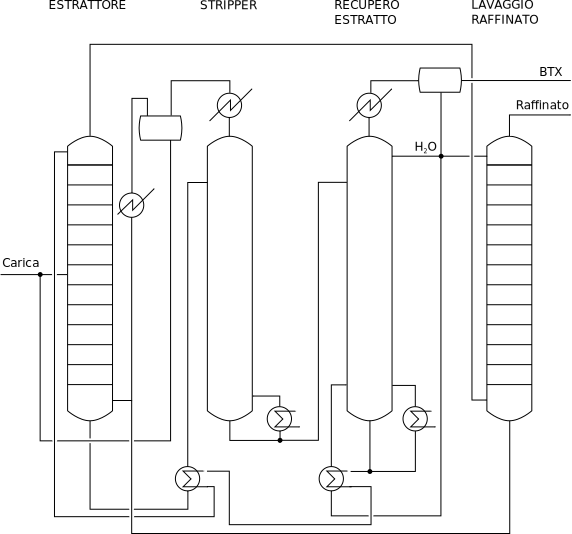
\includegraphics[width=0.80\textwidth]{image/ImpiantoBTX_SNAM}
	\caption{Rappresentazione dell'impianto SNAM}
	\label{fig:btx:SNAMPlant}
\end{figure}

\subsection{Processo IFP}
Il processo IFP\footnote{Istituto Francese Petroli} utilizza come solvente il dimetilsolfossido e l'estrazione viene compiuta in una colonna a piatti rotanti, dove � la forza centrifuga (gestibile dagli operatori) a far si che vi sia un flusso controcorrente.

Al posto dello stripping per il recupero del solvente si opera usando butano, che avendo densit� inferiore, far� si che il funzionamento sia a flussi invertiti (il solvente fuoriesce dall'alto della colonna). A seguito vi saranno una serie di colonne di lavaggio con acqua e di debutanazione per il recupero del flusso del'estrattore del dimetilsolfossido.

\subsection{Altri processi}
Il processo \textit{Lurgi} non passa attraverso una semplice estrazione dei BTX, ma si procede con una distillazione estrattiva, il cui solvente � composto da NMP\footnote{N-metilpirrolidone = \sixheterovi{3==N}{3==CH$_3$}}.
Anche in questo caso a seguito della distillazione estrattiva (dalla cui testa escono i composti non aromatici) si ha separazione dei BTX dal solvente tramite una rettifica.

Un'ulteriore tecnica utilizzata � la distillazione azeotropica in cui il solvente � costituito da metanolo che da luogo ad una miscela azeotropica con i composti non aromatici, si ha quindi una separazione di questi dagli aromatici. Il metanolo viene recuperato con acqua e successivamente separato (con notevoli costi energetici per l'intero processo). Questo procedimento viene adottato qualora la concentrazione del toluene sia superiore al 40\%.

\section{Separazione degli xileni}
Una volta ottenuta la miscela di BTX dalla prima separazione si pu� procedere alla distillazione per ottenere benzene, toluene e la miscela di xileni contenente anche etilbenzene e stirene. Da quest'ultima, per gli scopi dell'industria chimica, � necessario procede ad una ulteriore separazione dei componenti della miscela degli xileni e dell'etilbenzene, in particolare � necessario ottenere i tre differenti xileni\footnote{ovvero \textit{orto}, \textit{meta} e \textit{para} xilene}, l'etilbenzene e lo stirene puri. Data la vicinanza delle temperature di ebollizione e cristallizzazione delle diverse specie (\tablename~\ref{tab:btx:temperatureEbCr}) la separazione � assai difficoltosa, infatti per separare \ce{\textit{p}-xilene} e \ce{\textit{m}-xilene} servirebbe una colonna di circa 800 piatti. Non � nemmeno possibile procedere facilmente per estrazione data la somiglianza dei composti considerati (polarit� praticamente identiche), ma comunque possibile operare un adsorbimento frazionato.
\begin{table}[htbp]
	\centering
		\begin{tabular}{lcc} \hline
										& Ebollizione			& Fusione					\\ 
			Componente		&	$T_{eb}$, $^o$C	&	$T_{f}$, $^o$C	\\ \hline
			Etilbenzene		&	136.2						& -95.0						\\
			\textit{p}-xilene			& 138.3						& ~13.3						\\
			\textit{m}-xilene			& 139.1						& -47.9						\\
			\textit{o}-xilene			& 144.4						& -25.2						\\
			Stirene				& 145.2						& 								\\ \hline
		\end{tabular}
	\caption{Temperature di ebollizione e cristallizzazioen dei BTX}
	\label{tab:btx:temperatureEbCr}
\end{table}

\subsection{Cristalliazzazione frazionata }
Come � evidente da \figurename~\ref{fig:btx:cristallizzazione} la miscela si \textit{p}-xilene e \textit{m}-xilene pu� essere separata tramite cristallizzazione, ma si ha la formazione di un eutettico all'86\% composto da \textit{m}-xilene e di conseguenza una sola cristallizzazione non permette di ottenere una purezza del prodotto sufficiente. Per ovviare a ci� si pu� procedere ricristallizzando il prodotto iniziale o effettuando un lavaggio dei cristalli per eliminare il liquido intersitizale.
\begin{figure}[htbp]
	\centering
		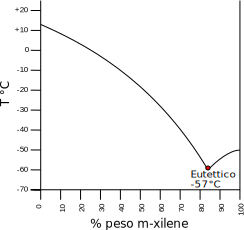
\includegraphics[width=0.60\textwidth]{image/eutettico}
	\caption{Temperatura di fusione del sistema \textit{p}-xilene \textit{m}-xilene}
	\label{fig:btx:cristallizzazione}
\end{figure}

La separazione mediante cristallizzazione viene realizzata in un impianto secondo un processo chiamato \textit{Phillips} in cui la separazione del liquido interstiziale dai cristalli di \textit{p}-xilene viene realizzato tramite ricristallizzazione e ulteriore rettifica, o in un impianto \textit{Atlantic} in cui si utilizza un solvente per eliminare dai cristalli di \textit{p}-xilene il liquido interstiziale (separati poi tramite rettifica).

\subsubsection{Impianto Phillips}
In questa tipologia di impianto (rappresentato in \figurename~\ref{fig:btx:phillipsPlant}) la miscela iniziale contenente i componenti aromatici $C_8$ viene inviata ad una prima colonna di distillazione (\textit{A}) composta da circa 150 piatti dalla cui coda si ottiene l'\textit{o}-xilene con una purezza sufficientemente elevata (circa il 98\%).

La testa della coda viene inviata ad una colonna di rettifica composta da circa 350 piatti (\textit{B}), chiamato anche \textit{superfrazionatore}\footnote{A volte si preferisce sostituire a questo un impianto per l'isomerizzazione da etilene a xileni.}, dalla cui testa si ottiene etilbenzene mentre dalla coda si ricava la miscela di meta e para xilene. Questa viene dapprima raffreddata fino ad una temperatura di circa $-23^oC$ (sfruttando il riscaldamento della miscela gi� raffreddata di recupero) e successivamente tramite un ciclo ad etilene fino a $-54^oC$.

La miscela cos� raffreddata viene inviata ad un filtro rotante dove si separano i cristalli di \textit{p}-xilene mentre la fase liquida � composta da \textit{m}-xilene che viene dapprima sottoposta ad una rettifica in una colonna da 200 piatti (\textit{C}) per recuperare altro etilbenzene dalla testa, mentre la coda viene inviata ad una altra colonna di rettifica di circa 50 piatti (\textit{D}) dalla cui testa si ricava \textit{m}-xilene al 95\%.

I cristalli di \textit{p}-xilene dopo una prima fusione vengono ricristallizzati e l'effluente inviato ad una colonna di rettifica (\textit{E}) dalla cui coda si ricava \textit{p}-xilene al 98\% e dalla cui testa si recupera una miscela di meta e para xileni che viene reciclata.

La colonna di purificazione \textit{E} pu� anche essere sostituita da una colonna a pistone con fondo riscaldato, in pratica un pistone preme sul fondo i cristalli in modo che i cristalli impuri si fondano alla base creando due gradienti, un primo di temperatura dal fondo verso la testa della colonna e del \textit{p}-xilene che tende verso il fondo della colonna (mentre il \textit{m}-xilene tende verso la testa).
\begin{figure}[htbp]
	\centering
		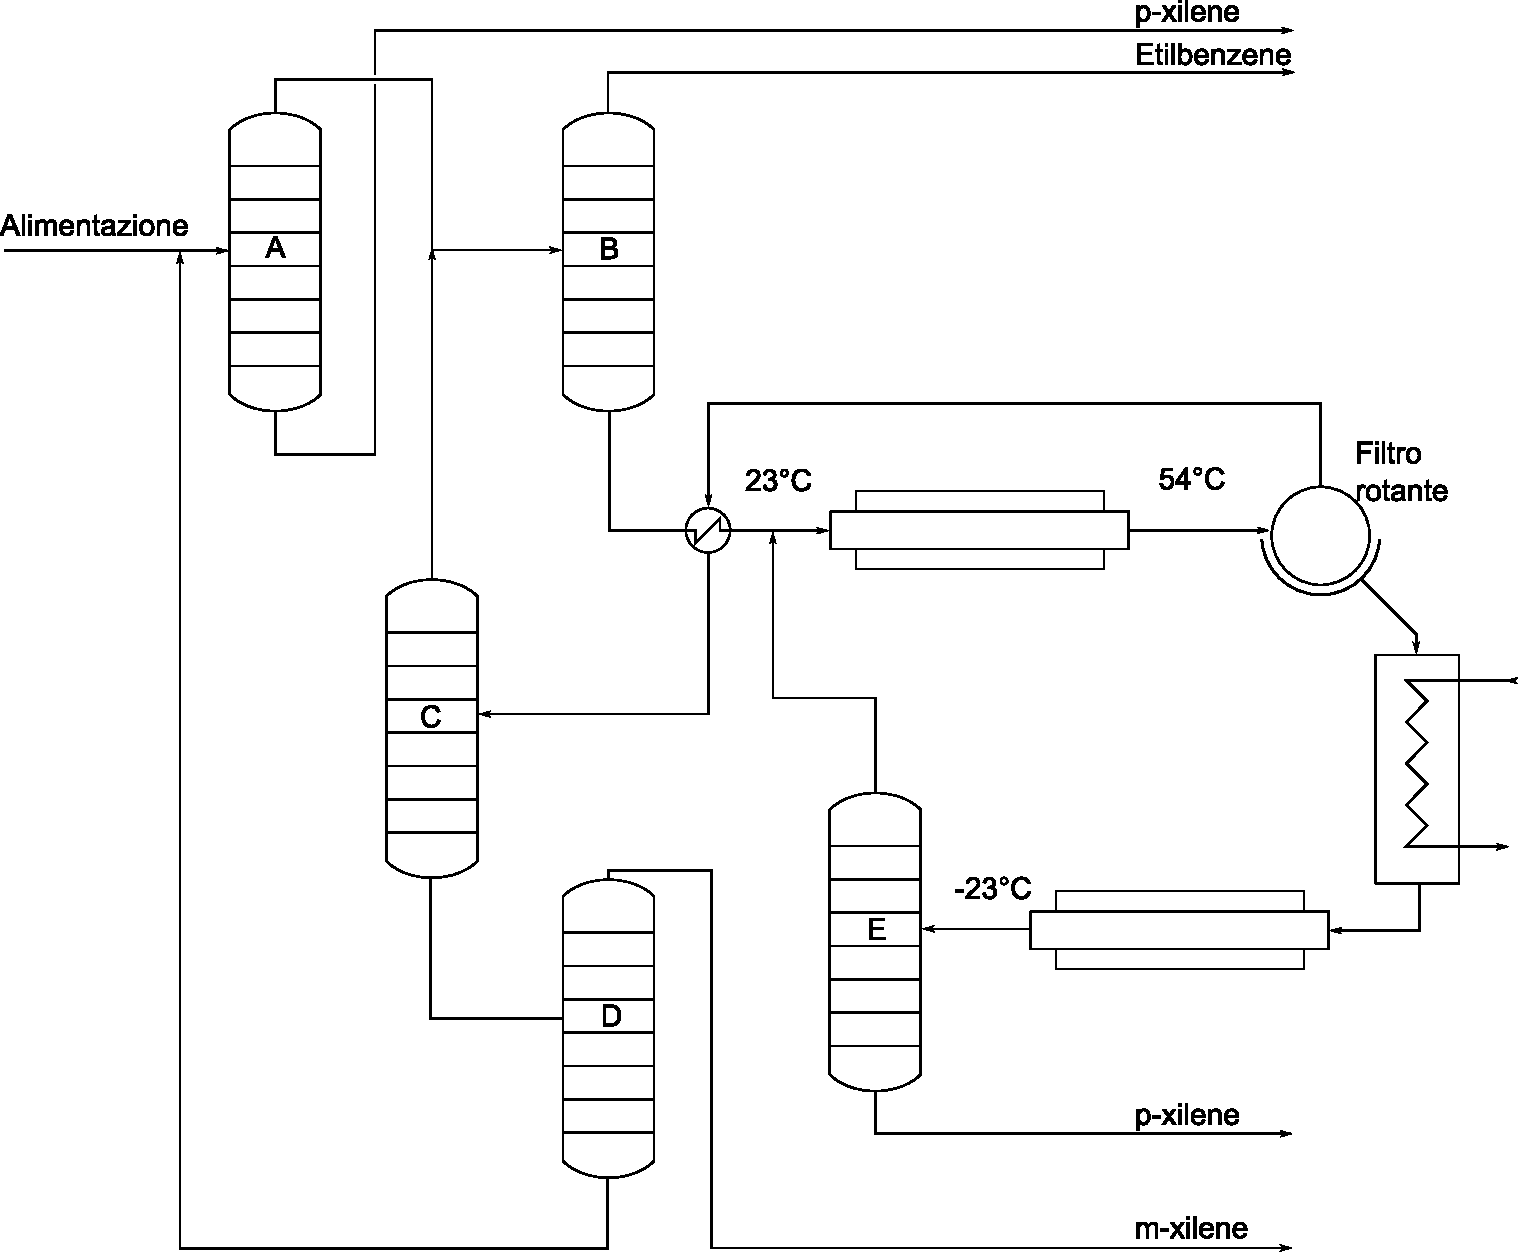
\includegraphics[width=0.90\textwidth]{image/phillipsPlant}
	\caption{Impianto per la separazione \textit{p}-xilene \textit{m}-xilene secondo il processo Phillips}
	\label{fig:btx:phillipsPlant}
\end{figure}

\subsubsection{Impianto Atlantic-Richfield}
In questa tipologia di impianto si procede alla separazione del \textit{p}-xilene dal \textit{m}-xilene non tramite ricristallizzazione e successiva rettifica, ma per mezzo di un lavaggio dei cristalli con toluene. Questo viene poi separato dal toluene tramite una rettifica.

\subsection{Adsorbimento frazionato}
In questo processo viene sfruttata la capacit� dei composti di adsorbire alcune sostanze, in questo caso particolare vengono usati dei setacci molecolari costituiti da \textit{silico-alluminati} con una microgeometria molto controllata.

Il \textit{p}-xilene riesce a penetrare nei setacci zeolitici, mentre il \textit{m}-xilene a causa degli ingombri sterici, non riesce a penetrare negli interstizi. Al termine di questo adsorbimento vengono separate le fasi liquide e solide (che hanno intrappolato il \textit{m}-xilene). Dai setacci si ha eliminazione del \textit{p}-xilene usando toluene come eluente, si ottiene cos� una soluzione di \textit{p}-xilene e toluene che poi verr� separata mediante rettifica. I setacci molecolari vengono poi rinviati alla fase di adsorbimento.

Questo schema ideale (\figurename~\ref{fig:btx:adsorbimentoFrazionatoIdeale}) sarebbe realizzabile se la fase contenente i setacci molecolari fossero liquida; il fatto che si tratti di una fase solida comporta una serie di problematiche che sono state risolte ricorrendo ad una configurazione chiamata SMB\footnote{Simulated Moving Bed}. In questo caso la colonna di adsorbimento/desorbimento � suddivisa in una serie di piatti e riempita da granuli di silico-alluminati. Ogni piatto conterr� un ingresso e una uscita e tutte queste sono collegate ad una valvola rotante.

La valvola rotante si occupa di modificare ciclicamente i flussi in ingresso e uscita da ogni piatto (alternativamente in ingresso si avr� la miscela di \textit{m}-xilene e \textit{p}-xilene oppure toluene e in uscita si avr� il raffinato o l'estratto), creando cos� un processo quasi continuo (idealmente continuo se il numero di piatti tende ad $\infty$).

Il raffinato, composto da \textit{m}-xilene non viene utilizzato tal quale ma subisce una isomerizzazione, reazione praticamente atermica, con catalizzatori acidi (zeolitici) e il prodotto verr� riciclato per ottenere il solo \textit{p}-xilene. La possibilit� di cracking dato dal catalizzatore utilizzato viene minimizzato aggiungendo idrogeno, che viene poi recuperato.

\begin{figure}[htbp]
	\centering
		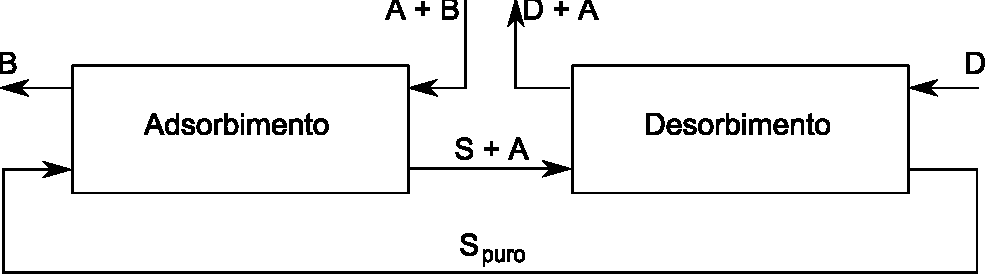
\includegraphics[width=0.90\textwidth]{image/adsorbimentoFrazionatoIdeale}
	\caption[Schema di un impianto di asorbimento frazionato ideale]{Schema di un impianto di asorbimento frazionato ideale. \textit{A}:~\textit{p}-xilene; \textit{B}:~\textit{m}-xilene; \textit{D}:~toluene; \textit{S}:~silico-alluminati}
	\label{fig:btx:adsorbimentoFrazionatoIdeale}
\end{figure}

\begin{figure}[htbp]
	\centering
		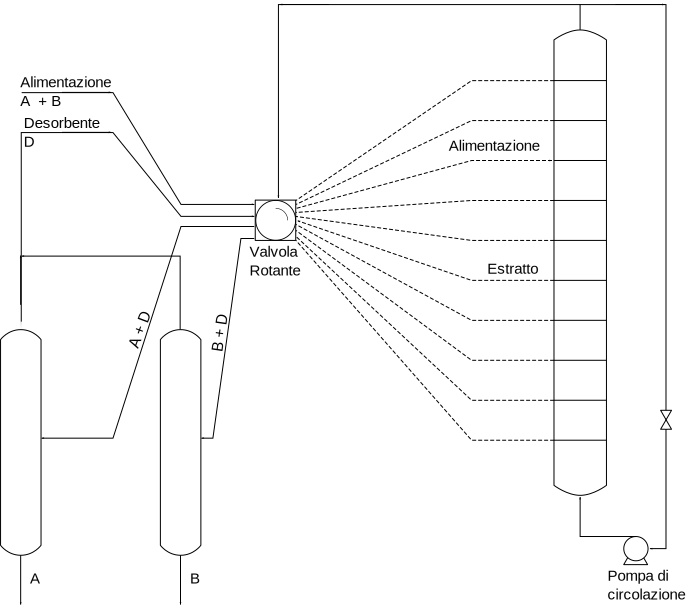
\includegraphics[width=0.90\textwidth]{image/adsorbimentoFrazionato}
	\caption[Schema di un impianto di asorbimento frazionato. Processo Parex]{Schema di un impianto di asorbimento frazionato secondo il processo \textit{Parex}. \textit{A}:~\textit{p}-xilene; \textit{B}:~\textit{m}-xilene; \textit{D}:~toluene;}
	\label{fig:btx:adsorbimentoFrazionato}
\end{figure}
	 \chapter{Separazione di miscele di idrocarburi}
I composti idrocarburici a basso peso molecolare ottenuti all'uscita del processo di steam cracking devono essere separati per poter essere utilizzati. La miscela di partenza ha una composizione simile a quella indicati in \tablename~\ref{tab:si:conposizioneSC}. Dati gli ingenti quantitativi di gas da trattare le uniche tecniche adottabili economicamente vantaggiose sono i frazionamenti per mezzo di distillazione o per lavaggio con solventi. 
\begin{table}[htbp]
	\centering
		\begin{tabular}{lc} \hline
		Prodotto												& contenuto	\\ \hline
		Idrogeno												& 1-2 \%		\\
		Metano													& 10-18 \%	\\
		Etilene													& 20-35 \%	\\
		Propilene												& 12-18 \%	\\
		Frazione $C_4$									& 7-13 \%		\\
		Benzene													& 6-7 \%		\\
		Frazione $C_5$ e aromatici			& 5-10 \%		\\ \hline
		\end{tabular} 
	\caption{Composizione del flusso in uscita dallo Steam Cracking}
	\label{tab:si:conposizioneSC}
\end{table}

Il problema maggiore nell'utilizzo del frazionamento per distillazione � dato dalle basse temperature di ebollizione dei composti leggieri e dalla vicinanza delle temperature di ebollizione di alcuni composti (vedi \tablename~\ref{tab:si:caratteristicheCH})
\begin{table}[htbp]
	\centering
		\begin{tabular}{p{3cm}ccc} \hline
		Composto			& $T_{eb} (^oC)$ & $T_{critica} (^oC)$ & $P_{critica} (Atm)$ \\ \hline
		\ce{H_2}			&		-252.5			 & 			-239.8				 &			13.2					 \\
		\ce{N_2}			&		-195.8			 & 			-147.1				 &			33.5					 \\
		\ce{CO}				&		-191.5			 & 			-140.2				 &			34.5					 \\
		\ce{CH_4}			&		-161.5			 & 			-82.3					 &			45.8					 \\
		\ce{C_2H_4}		&		-103.8			 & 			9.7						 &			50.7					 \\
		\ce{C_2H_6}		&		-88.6				 & 			33.0					 &			48.6					 \\
		\ce{C_2H_2}		&		-83.6			 	 & 			35.7					 &			81.6					 \\
		\ce{C_3H_6}		&		-47.7			 	 & 			91.4					 &			45.4					 \\
		\ce{C_3H_8}		&		-42			 		 & 			95.8					 &			41.6					 \\
		\ce{iso-C_4H_{10}}&-11.7			 & 			133.8					 &			30.2					 \\
		\ce{n-C_4H_8}	&		-6.26			 	 & 			144.1					 &			37.5					 \\
		\ce{n-C_4H_{10}}&	-0.5			 	 & 			152.0					 &			37.5					 \\
		\ce{1,3 C_4H_6}&	-4.4			 	 & 			163.0					 &			42.1					 \\ \hline
		\end{tabular}
	\caption{Caratteristiche fisiche delle frazioni idrocarburiche leggere}
	\label{tab:si:caratteristicheCH}
\end{table}

\section{Impianto di frazionamento tramite rettifica}
Un impianto generico per il frazionamento di questi composti � formato da quattro colonne di rettifica che separano le frazioni \ce{H_2} e \ce{C_1}, \ce{C_2H_4}, \ce{C_2H_6}, \ce{C_3} e come ultima frazione rimanente \ce{C_4} e \ce{C_5}. Lo schema � visibile in \figurename~\ref{fig:si:impiantoFrazionamentHC}.

\begin{figure}[p]
	\centering
		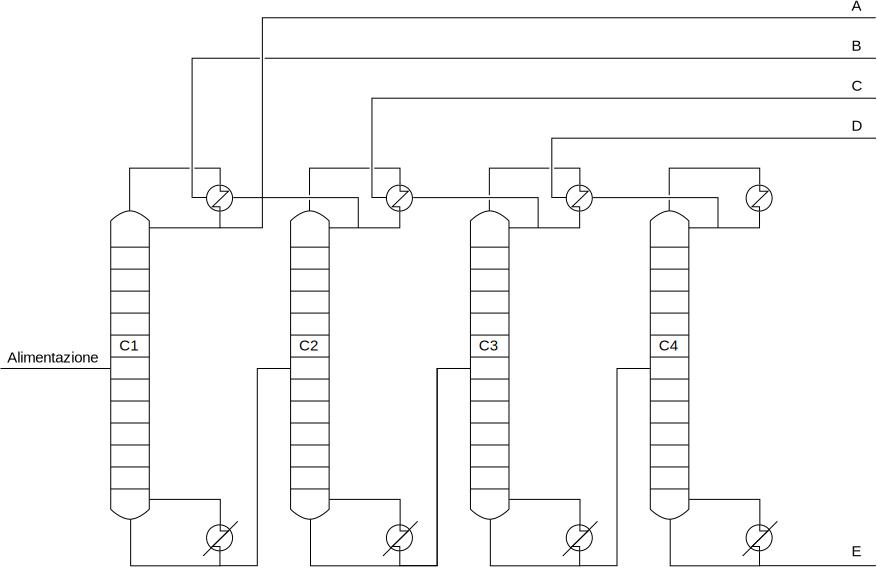
\includegraphics[width=0.90\textwidth]{image/impiantoFrazionamentHC}
	\caption[Impianto di frazionamento degli idrocarburi a basso PM]{Impianto di frazionamento degli idrocarburi a basso PM. \textit{A}: \ce{C_1} e \ce{H_2}; \textit{B}: \ce{C_2H_4}; \textit{C}: \ce{C_2H_6}; \textit{D}: \ce{C_3}; \textit{E}: \ce{C_4} e \ce{C_5};}
	\label{fig:si:impiantoFrazionamentHC}
\end{figure}

L'impianto indicato � composta da quattro colonne ed ognuna di esse opera in condizioni tali per cui il refrigerante che deve giungere alla testa della colonna � composto dal fluido di testa della colonna successiva che viene fatto espandere e sottrae il calore necessario a condensare i vapori di testa della colonna di rettifica. Le condizioni operative delle colonne indicate in \figurename~\ref{fig:si:impiantoFrazionamentHC} sono indicate in \tablename~\ref{tab:si:impiantoFrazionamentHC:CondizOperative}

\begin{table}[p]
	\centering
		\begin{tabular}{lcccc} \hline
		Colonna												& C1	&  C2 & C3 & C4 \\ \hline
		Pressione (Atm)								&	 40	&	 27 & 24 & 15 \\
		Temperatura di testa ($^oC$))	& -90	&	-18 &  4 & 38 \\
		Temperatura di coda ($^oC$))	&  38	&	 43 & 65 & 93 \\ \hline
		\end{tabular}
	\caption{Condizioni operative dell'impianto di separazione degli idrocarburi a basso PM}
	\label{tab:si:impiantoFrazionamentHC:CondizOperative}
\end{table}

I titoli di testa dele colonne \textit{C2} e \textit{C3} non � elevato e si attesta su di un valore del 95\% circa, mentre dalla testa della colonna \textit{C1} si trova, oltre alle specie cercate anche un elevato tenore di etilene.

L'intero impianto non pu� operare se vengono superate le temperature critiche dei diversi composti nelle diverse colonne, quindi la temperatura di testa della colonna \textit{C1} non pu� mai superare la temperatura critica del metano ($-90^oC$) altrimenti non si avrebbe condensazione della testa, il riflusso nei piatti di testa sarebbe nullo e la colonna non potrebbe operare come colonna di rettifica. Sarebbe persino possibile abbassare la pressione operativa delle diverse colonne, tuttavia ci� porterebbe ad avere la necessit� di operare a temperature ancora inferiori, facendo crescere i costi necessari alla sottrazione del calore; e dato che le condizioni operative sono tali da necessitare di un buon isolamento tutte le colonne sono coibentate e si ha un recupero termico tra le colonne stesse.

Altro problema che sorge (sempre nella colonna \textit{C1}) � dato dalla necessit� di far si che le condizioni a fondo colonna non superino le condizioni critiche del propilene, infatti verrebbe pregiudicata la presenza di questo in fase liquida; per questo motivo non � possibile avere pressioni superiori a 40atm e la presenza della fase liquida � molto precaria, poich� piccole variazioni della temperatura portano ad una diversa condensazione e pertanto la regolazione del processo � difficoltosa.

\section{Separazione etano - etilene}
L'etilene ottenuto dalla prima distillazione si trova ad un grado di purezza tale per cui il suo utilizzo non � consentito, bisogna quindi andare a purificarlo per ottenere una purezza superiore, in modo che possa essere utilizzato.

Data la differenza di temperatura tra le due specie considerate (circa $15^oC$) e la natura del diagramma liquido vapore si pu� effettuare la separazione tramite una unica colonna di rettifica. In questo caso si opera in modo da avere, come refrigerante di testa l'etilene che viene espanso isoentalpicamente da 6atm a 1atm sottraendo il calore necessario alla condensazione, oppure dell'etano di coda da 15-20atm a 1atm.

In queste condizioni � sufficiente una colonna da 100 piatti e un rapporto di riciclo di 3-4, per avere (considerando una concentrazione di acetilene pressoch� nulla, poich� si � effettuata una idrogenazione in modo da eliminarlo) una concentrazione di etilene del 99.9\%, ovvero suffciente a poter essere utilizzato per il processo di polimerizzazione con sistemi Zigler-Natta.

\section{Separazione propano - propilene}
La separazione della frazione \ce{C_3} viene effettuata separando il propano dal propilene, ma poich� la differenza delle temperature di ebollizione di questi due composti sono molto basse ($5.7^oC$) la volatilit� relativa tende al valore unitario e di conseguenza la separazione � abbastanza difficoltosa. Operando ad una pressione di 20atm, in modo che in testa sia possibile utilizzare acqua come refrigerante, � necessario disporre di una colonna di 130piatti teorici per ottenere un purezza dei prodotti superiore al 99\%. 

A pressioni inferiori si potrebbero utilizzare colonne pi� corte, ma necessiterebbero di usare come refrigerante il propilene liquido. Altro metodo utilizzabile per diminuire le dimensioni della colonna da utilizzare � l'inserimento di un terzo composto polare che abbassi la volatilit� relativa del propilene rispetto al propano. Come solventi possono essere utilizzati furfurolo (eventualemente con aggiunta di alcuni punti percentuale di acqua), acrilonitrile, acetonitile o miscele di quest'ultimi.

Il processo pi� diffuso prevede l'utilizzo di una colonna a 20atm con refrigerante ad acqua e con 120-130piatti. La necessit� di utilizzare una colonna di tali dimensioni comporta notevoli problemi di stabilit� meccanica del dispositivo, si opta quindi per l'utilizzo di due colonne disposte in serie in modo da avere strutture pi� compatte e stabili. Un impianto di questo tipo � rappresentato in \figurename~\ref{fig:si:impiantoFrazionamentoC3}
\begin{figure}[htbp]
	\centering
		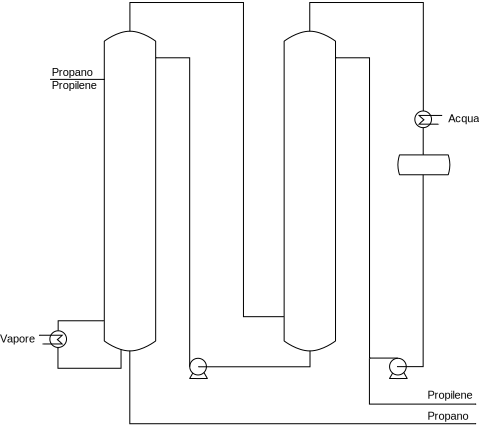
\includegraphics[width=0.70\textwidth]{image/impiantoFrazionamentoC3}
	\caption{Impianti di separazione propano - propilene}
	\label{fig:si:impiantoFrazionamentoC3}
\end{figure}

\section[Separazione della frazione C4]{Separazione della frazione \ce{C_4}}
Le miscele di \ce{C_4} ottenute da processi quali steam cracking, cracking termico, deidrogenazioni di \textit{n}-butano, etc contengono una miscela dei diversi isomeri e le rispettive olefine (vedi \tablename~\ref{tab:si:isomeriC4}), di conseguenza � necessaria una separazione per poter ottenere le diverse specie utilizzate nelle fasi successive.

\begin{table}[htbp]
	\centering
		\begin{tabular}{ccc}
			$\tetramethylene{}{}$ 					& $\tetramethylene[a]{}{}$ 			& $\tetramethylene[b]{}{}$  \\
					n-butano	  								& 		1-butene	 								& trans-2-butene						\\
			$\trimethylene[b]{}{3S==\null}$ & $\trimethylene{}{2S==\null}$ 	& $\trimethylene[b]{}{2S==\null}$	\\
					cis-2-butene	 							& 		iso-butano	 							& iso-butene								\\
			                         				& $\tetramethylene[ac]{}{}$ 		&                           \\
			               									& 		1-3butadiene	 						&		                    		\\
		\end{tabular}
	\caption{Isomeri delle specie C4}
	\label{tab:si:isomeriC4}
\end{table}

I prodotti principali desiderati sono i \textit{butadieni}, usati per al produzione di elastomeri, l'\textit{isobutene} usato per la produzione di MTBE, l'\textit{1-butene} per la produzione di poliolefine, l'\textit{\textit{n}-butano} e \textit{\textit{n}-butene} per la produzione di anidride maleica.

La separazione tra questi composti � alquanto difficoltosa, poich� le temperatura di ebollizione sono molto vicine e vi � la presenza di alcuni azeotropi di minima (in particolare tra butadiene e \textit{n}-butano), che rendono difficoltosa la separazione tramite semplice rettifica, infatti per la separazione della miscela \ce{1-butene}~/~\ce{cis 2-butene} per ottenere una purezza sufficientemente alta (99\%) � necessario operare con colonne di circa 110 piatti e un rapporto di riflusso pari a 45. Data una media produzione annua di 50000 tonnellate il dimensionamento della colonna porta ad avere un diametro di 1.9m e altezza di circa 90m, da cui il rapporto (detto snellezza) � pari a 47. Cio porta a notevoli problematiche costruttive, ma anche operative, inquanto anche piccole oscillazioni impediscono sulla testa l'orizzontalit� dei piatti e di conseguenza l'efficienza. Anche in questo caso � possibile operare usando pi� colonne in serie (come per il propilene).

\subsection{Distillazione estrattiva}
Per migliorare la rettifica della miscela iniziale si usano solventi polari, che data la diversa struttura elettronica dei composti olefinici (e di conseguenza la polarit� e polarizzabilit�), fa si che la volatilit� relativa degli idrocarburi insaturi sia minore di quella degli idrocarburi saturi (l'$\alpha$ diventa sufficientemente diversa da 1).

Le caratteristiche che il solvente deve avere sono l'elevata polarit�, (con elevata capacit� e selettivit�), in modo da ridurre la velocit� di ricircolazione e di conseguenza diminuire le dimensioni delle apparecchiature e i consumi energetici operativi. Una temperatura di ebollizione elevata rispetto al componente estratto in modo da facilitare la fase successiva di separazione dell'estratto; � necessario, inoltre, che possegga una certa stabilit� termica per evitare degradazione nei diversi cicli di utilizzo e ovviamente un costo sufficientemente basso da giustificarne l'impiego. Come specie solventi con le caratteristiche richieste sono state individuate alcune specie che sono anche quelle pi� utilizzate; queste sono indicate in \tablename~\ref{tab:si:solventiDistEstrattiva}.
\begin{table}[htbp]
	\centering
		\begin{tabular}{cc}
			$\vcenter{\hbox{\fiveheterov[A]{1==O}{2==CHO}}}$ &
			$\vcenter{\hbox{\fiveheterov[A]{1==N}{1==CH$_3$;2D==O}}}$ \\
			furfurolo &
			NPM = N-Metil Pirrolidone	\\
			$\vcenter{\hbox{\tetramethylene{1==CH$_3$;4==NH$_2$}{2==CH$_3$;3D==O}}}$ &
			$\vcenter{\hbox{$CH_3-C \equiv N$}}$ \\
			DMAC = dimetil acetamide &
			ACN = acetonitrile \\
		\end{tabular}
	\caption{Solventi utilizzati nella distillazione estrattiva delle specie \ce{C_4}}
	\label{tab:si:solventiDistEstrattiva}
\end{table}

\subsection{Alternative alla rettifica}
Oltre al meccanismo di rettifica (e rettifica estrattiva) � possibile operare utilizzando dei solventi particolarmente affini a determinate specie, per esempio l'isobutene ha una sua distribuzione delle cariche decisamente differente rispetto ad un n-butano e di conseguenza potrebbe essere possibile trovare un solvente (presumibilmente polare) che � molto pi� affine verso questa specie.

Potrebbero essere sfruttati anche fenomeni di adsorbimento selettivo sfruttando diversit� steriche delle specie considerate e di conseguenza operare con setacci molecolari per la separazione delle diverse sostanze (come per il caso della separazione del \textit{m}-xilene e \textit{p}-xilene). Per esempio la struttura del iso-butano � decisamente differente dal punto di vista degli ingombri sterici dal n-butano.

\subsection{Separazione del butadiene}
Il processo di separazione delle specie \ce{C_4} viene affrontato iniziando a sottrarre dalla miscela iniziale il butadiene, infatti questa � la specie che potrebbe comportare maggiori problemi nelle fasi successive, poich� date le sue caratteristiche potrebbe portare a polimerizzazione delle code delle diverse colonne di rettifica provocando degradazione del prodotto e danni alle colonne (intasamento). Inoltre � possibile la trasposizione degli idrogeni per portare a prodotti acetilenici (triplo legame) che essendo prodotti particolarmente esplosivi hanno come conseguenza un elevato rischio per le apparecchiature, oltre alla perdita della qualit� del prodotto.

La fase successiva prevede la separazione dell'isobutene dalla miscela rimanente, sia per ottenere il prodotto puro che per ottenere altre specie da esso derivato (MTBE).

\subsubsection{Processo Phillips (estrazione con furfurolo)}
Inizialmente (anni '40) il butadiene veniva estratto tramite un processo di distillazione estrattiva usando come solvente il furfurolo ($T_{eb} = 162^oC$). L'intero processo � composto da tre elementi principali, in una prima colonna di rettifica si ha eliminazione dalla testa, tramite l'immissione del furfurolo, delle specie $C_3$ presenti, dei butani e dei buteni. Un secondo elemento � lo stripper da cui si ha separazione dei gas adsorbiti nel furfurolo dei gas; dalla coda di questo elemento si ottiene furfurolo che dopo un raffreddamento e una fase di purificazione viene reimmesso nella colonna principale, mentre dalla testa si ottiene l'1,3-butadiene e altri buteni che vengono poi separati da una seconda colonna di rettifica. Lo schema di processo � visibile in \figurename~\ref{fig:si:butadienePhillips}.
\begin{figure}[htbp]
	\centering
		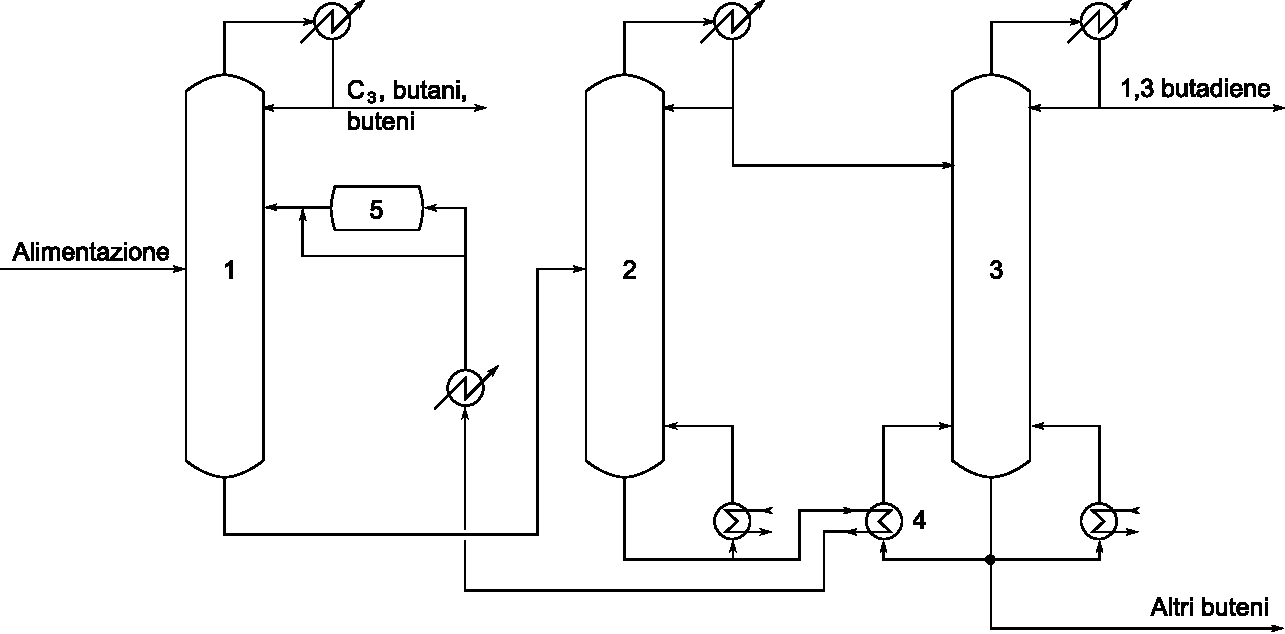
\includegraphics[width=0.90\textwidth]{image/butadienePhillips}
	\caption[Impianto per l'ottenimento di butadiene (processo Phillips)]{Impianto per l'ottenimento di butadiene (processo Phillips). \textit{1}: colonna di rettifica estrattiva; \textit{2}: Stripper; \textit{3}: Colonna di rettifica finale; \textit{4}: raffreddamento del furfurolo; \textit{5}: Purificazione del furfurolo.}
	\label{fig:si:butadienePhillips}
\end{figure}

\subsubsection{Processo Shell (estrazione con ACN)}
Dagli anni '60 si afferma il processo Shell in cui la carica viene dapprima inviata ad una colonna di rettifica estrattiva con solvente a base di ACN\footnote{Acetonitrile.}. Dalla testa si ottiene la miscela di butani e buteni, mentre dalla coda si estrae il solvente contenente l'1,3-butandiene. Questo viene inviato a uno stripper dove si ha separazione del solvente (che verr� riciclato alla prima colonna) e dei gas che contengono alcuni gas leggeri e gli 1,3-butadieni. questa miscela gassosa viene dapprima inviata ad una colonna di rettifica dove si separano i gas leggeri dalla testa, mentre i butadieni (che escono dalla coda) vengono inviati ad una seconda colonna di rettifica dove vengono separati dai composti pesanti che sono presenti.

I composti pesanti, e i gas uscenti dalla testa della prima rettifica vengono inviati ad una colonna per lavaggio con acqua per il recupero del'ACN trascinato, e successivamente escono dall'impianto. La miscela ACN acqua viene invece inviata ad una colonna di rettifica che procede alla separazione dei due componenti, l'ACN torna alla colonna primaria per la rettifica estrattiva, mentre l'acqua viene riciclata alla colonna di lavaggio. Lo schema dell'impianto � visibile in \figurename~\ref{fig:si:butadieneShell}.
\begin{figure}[p]
	\centering
		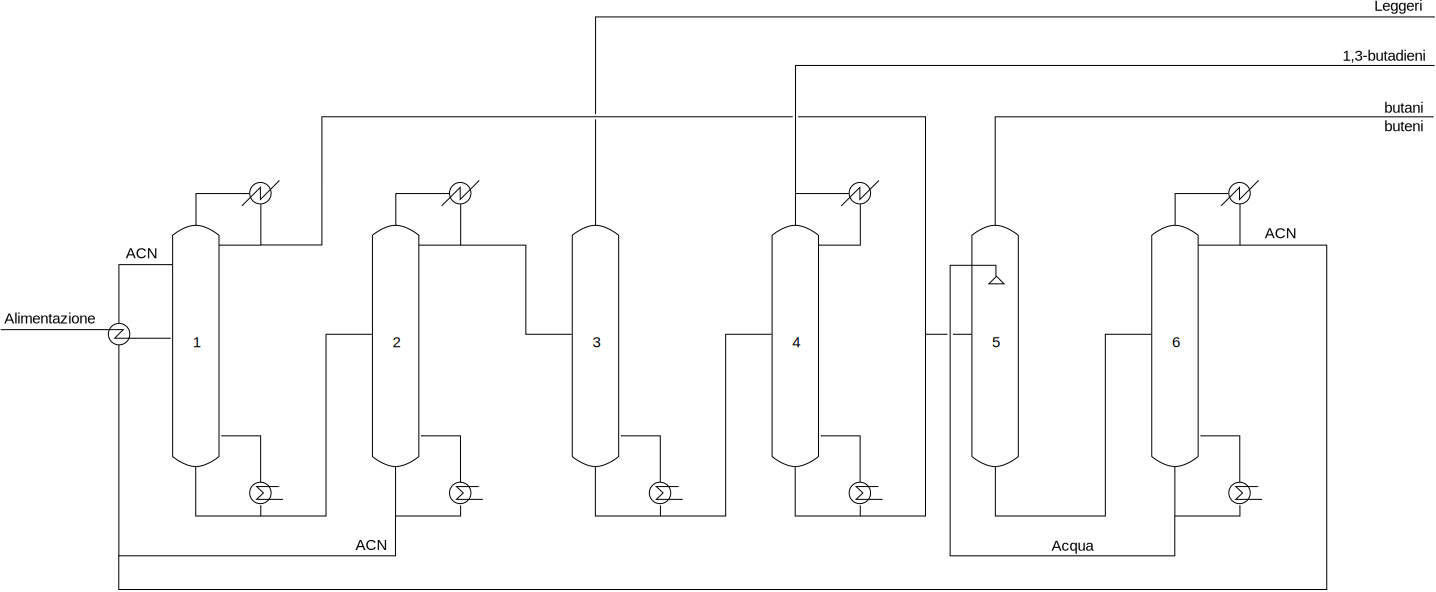
\includegraphics[angle=90,height=0.93\textheight]{image/butadieneShell}
	\caption[Impianto per l'ottenimento di butadiene (processo Shell)]{Impianto per l'ottenimento di butadiene (processo Shell).
	\textit{1}: Colonna di rettifica estrattiva;
	\textit{2}: Stripper del solvente;
	\textit{3}: Colonna di rettifica dei leggeri; 
	\textit{4}: Colonna di rettifica per i butandieni;
	\textit{5}: Colonna di lavaggio;
	\textit{6}: Colonna di separazione ANC e Acqua;}
	\label{fig:si:butadieneShell}
\end{figure}

\subsubsection{Processo Union Carbide (estrazione con DMAC)}
Questo processo � molto simile a quello sviluppato dalla Shell e usa come solvente il DMAC\footnote{Dimetil acetamide}. In questo caso vi sono due colonne di rettifica estrattiva e due stripper che lavorano in sequenza seguiti poi da due colonne di rettifica in serie per la separazione dell'1,3-butandiene dal resto dei composti estratti dal solvente.

Il vantaggio di questo processo � dato dalla riduzione di temperatura della distillazione estrattiva, limitando quindi le polimerizzazione del butadiene e le problematiche ad esso connesse.

\subsubsection{Processo BASF (estrazione con NMP)}
Il processo BASF utilizza il NMP\footnote{N-metil pirrolidone} per l'estrazione del butadiene dagli altri \ce{C_4}, dopo una fase iniziale di riscaldamento degli idrocarburi e dei prodotti di ricilo vengono inviati in una colonna di adsorbimento dove si ha, in controcorrente, un flusso di NMP. Segue poi una zona in cui si ha una smiscelazione e un primo scrubber dove si separano i butandieni dal solvente.

Un secondo stripper, che preleva dal fondo dello smiscelatore la miscela di NMP pi� ricca di acetileni, separa il sovente che viene riciclato dai gas, che vengono inviati ad una colonna di lavaggio ad acqua e successivamente ad un idrogenatore che trasforma gli alchini in alcheni. La miscela uscente da questo viene reinviata all'alimentazione della prima colonna per poter recuperare gli alcheni cos� ottenuti.

\subsubsection{Processo ESSO (estrazione con CAA)}
Il processo Esso sfrutta una soluzione cuproammoniacale. Le olefine formano con questo un complesso labile che pu� essere facilmente decomposto per semplice riscaldamento, si ha quindi una prima operazione di estrazione usando una colonna dalla cui testa viene inserita la soluzione cuproammoniacale, mentre dalla coda viene alimentato il gas di partenza.
All'uscita della colonna di estrazione si ottengono butani e buteni dalla testa, mentre la soluzione contenente dieni viene dapprima riscaldata per ottenere la dissociazione del complesso e successivamente inviata ad una serie di colonne di distillazione per il recupero del solvente dai \ce{C_4} insaturi.
L'intero impianto opera a bassa pressione e permette la separazione anche con piccole percentuali di 1,3-butadiene.

\subsection{Separazione del isobutene}
La fase successiva alla separazione del butadiene dalla miscela alimentata prevede la separazione dell'isobutene dalla miscela rimanente, sia per ottenere il prodotto puro che per ottenere altre specie da esso derivato (MTBE).

\subsubsection{Separazione con acido solforico}
Date le particolari caratteristiche elettroniche dell'isobutene questo pu� essere separato in maniera selettiva dagli altri idrocarburi \ce{C_4} per semplice estrazione con una soluzione di acido solforico al 40-50\%. La reazione � esotermica e viene dunque condotta a una temperatura bassa, in genere tra 20 e $50^oC$. La reazione � la seguente:
\begin{equation}
		\vcenter{\hbox{\trimethylene[a]{}{2S==\null}}} + H_2SO_4
		\stackrel{^{\lambda}}{\rightleftharpoons}
		\vcenter{\hbox{\trimethylene{}{2S==\null;3W==OSO$_3$H}}}
\end{equation}
Una volta effettuato l'assorbimento i due componenti possono essere rigenerati per semplice riscaldamento e successivamente separati mediante lavaggio con acqua. L'acido solforico cos� ottenuto viene concentrato tramite rettifica e reinviato nella colonna di estrazione.

Purtroppo il processo cos� congeniato ha degli elevati costi di produzione, infatti � necessario effettuare il riscaldamento del \textit{solfato acido terz-butossido} per ottenere la separazione dei due componenti di partenza, inoltre � necessario riconcentrare l'acido solforico e le apparecchiature devono essere realizzate in acciaio resistente all'acido solforico; infine si hanno anche elevati problemi ambientali, quindi � sempre meno utilizzato come processo per la separazione.

\subsubsection{Processi di separazione moderni}
Attualmente il processo di separazione pi� utilizzato � l'esterificazione dell'isobutene a MTBE\footnote{\textit{Metil terzbutil ossido}, prodotto che ha sostituito il piombo tetraetile nelle benzine come antidetonante, quindi molto richiesto dall'industria petrolchimica.} aggiungendo metanolo o la semplice idratazione a dare terzbutanolo che pu� essere riconvertito, in caso di necessit�, a isobutene tramite disidratazione.

Uno impianto che sfrutta queste tecnologie � il processo H\"uls in cui le due tecnologie vengono impiegate entrambe e i prodotti ottenuti vengono scelti in funzione delle richieste del mercato.
	 \chapter{Sintesi dell'MTBE}
L'MTBE\footnote{Metil \textit{Terz}-Butil Etere} � una sostanza che negli ultimi decenni ha subito un notevole sviluppo grazie ad alcune sue caratteristiche che lo hanno portato a sostituire il piombo tetraetile, sostanza altamente tossica poich� contiene un metallo pesante e nociva per i catalizzatori delle marmitte, come antidetonante nelle benzine. Il suo impiego in questo settore ha fatto si che la sua produzione sia stata quella a pi� alto tasso di crescita negli anni ottanta, portandolo a produzioni paragonabili a quelle delle olefine (etilene, propilene, ...), tanto da raggiungere la posizione 12 nelle \textit{top 50} delle sostanze pi� prodotti in USA nel 1995.

I vantaggi che hanno portato la scelta dell'MTBE come sostituto del \ce{Pb(Et)_4} nelle benzine sono duplici, da un lato l'utilizzo dell'MTBE porta ad un innalzamento del numero di ottano della miscela, permettendo di avere motori con rapporti di compressione maggiori e di conseguenza consumi ridotti fungendo anche da fornitore di ossigeno e migliorando la combustione. Altro fattore rilevante per la scelta di questa sostanza � il costo di produzione che non � totalmente legato al valore del greggio (il prezzo dipende anche dal metanolo, prodotto a basso costo). Come fornitore di ossigeno nella miscela possono essere utilizzate anche altre sostanze, quali alcoli (Etanolo, TBA\footnote{\textit{terz}-butanolo}), eteri (TAME\footnote{teramil-metil-etere}, TAEE\footnote{teramil-etil-etere}, DIPE\footnote{di-isopropil-etere}) con la differenza che questi hanno un costo maggiore e non aumentano il numero di ottano quanto l'MTBE. Da considerare che le benzine riformulate (in America pari a circa il 32\% della benzina erogata) � obbligatoria una presenza di ossigeno pari al 2\%, ma per raggiungere tali valori � necessario che sia presente l'11\% di MTBE; ci� pu� far capire l'importanza di questo prodotto, che in America � passato da 10MTPY\footnote{Milion Tons Per Year = milioni di tonnellate annue} del 1991 al 24MTPY del 1996 con un treand in continua crescita. Negli anni '90 si � scoperto in California (USA), dove l'uso di MTBE � massiccio e pari a circa il 40\% del consumo americano, che questa sostanza pu� provocare inquinamento delle falde acquifere, essendo scarsamente biodegradabile; per questo motivo, e una sua presnta tossicit�, negli ultimi anni si sta cercando un degno sostituto.

\section{Sintesi}
\subsection{Il meccanismo di reazione}
La sintesi dell'MTBE � abbastanza semplice, infatti si tratta di una reazione in cui del metanolo e dell'isobutene vengono miscelati in presenza di un catalizzatore acido. Questo lega a se l'\ce{iso-butene} scindendo il doppio legame e creando cos� una parziale carica positiva. L'ossigeno del metanolo possiede due doppietti elettronici liberi che hanno cariche parziali negative, di conseguenza viene attratto dall'isobutano legato al catalizzatore e si ha formazione dell'MTBE.

La reazione complessiva � moderatamente esotermica ($\Delta H$= -10Kcal/mol) e controllata dall'equilibrio; per questo motivo si opera a temperature sufficientemente basse (circa $50-80^oC$) e con una pressione di qualche atmosfera cos� da mantenere l'MTBE in fase liquida ($T_{eb} = 82^oC$).

I sottoprodotti che si possono formare sono eteri dimetilici dalla condensazione di due molecole di metanolo, il \ce{di-iso-butene} dalla reazione di due molecole di butene e l'alcool terz-butilico.

\subsection{L'impianto}
Come reagenti vengono utilizzati le miscele di \ce{C_4} e metanolo, poich� la selettivit� verso l'isobutene � talmente elevata da permettere di avere comunque una purezza spinta e una conversione dell'\ce{iso-butene} praticamente unitaria. Si ha, quindi, una prima zona in cui avviene il lavaggio della frazione \ce{C_4} (gi� privata del butadiene) con acqua per eliminare eventuali impurezze che possono danneggiare il catalizzatore, una seconda zona in cui avviene la reazione tra \ce{iso-butene} e \ce{metanolo} e la successiva separazione dell'MTBE dai gas rimanenti. La separazione prosegue estraendo il metanolo non reagito con acqua e facendo seguire il tutto da uno stripper (o rettifica) per ottenere la separazione del metanolo dall'acqua di estrazione.

La zona di reazione � composta da due reattori, il primo in cui avviene il grosso della produzione di MTBE a cui segue una colonna di separazione per estrarre il grosso dell'MTBE e un secondo di raffinazione del processo in cui si ha la completa conversione dell'\ce{iso-butene}. Lo schema � rappresentato in \figurename~\ref{fig:mtbe:Plant}.

\begin{figure}[htbp]
	\centering
		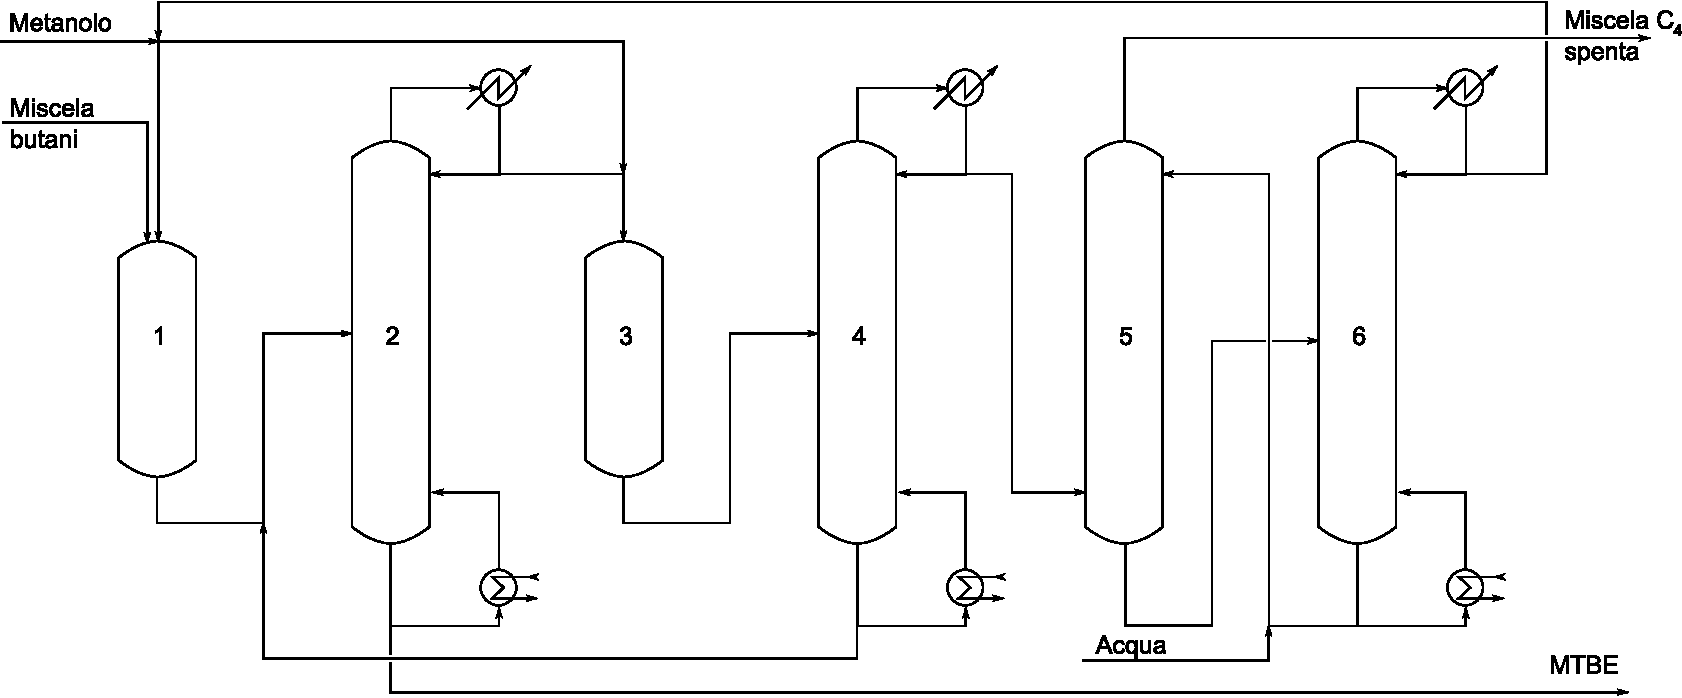
\includegraphics[width=0.95\textwidth]{image/mtbePlant}
	\caption[Schema dell'impianto per la produzione di MTBE]{Schema dell'impianto per la produzione di MTBE. 
	\textit{1}: Primo reattore;
	\textit{2}: Rettifica per la separazione dell'MTBE;
	\textit{3}: Secondo reattore;
	\textit{4}: rettifica per recupero MTBE;
	\textit{5}: Colonna di lavaggio con acqua;
	\textit{6}: Separazione metanolo-acqua;
	}
	\label{fig:mtbe:Plant}
\end{figure}

\subsection{I reattori}
La produzione di MTBE pu� avvenire in diverse tipologie di reattori, attualmente le tipologie utilizzate sono le quattro elencate di seguito.

\subsubsection{Reattore adiabatico}
E' il reattore pi� semplice da realizzare, inizialmente si ha una rapida crescita della temperatura parallela alla conversione dei reagenti in MTBE, fino a quando non viene raggiunto un punto di equilibrio. Il reattore deve essere sovra dimensionato per ovviare ai problemi di disattivazione del catalizzatore, inoltre la parte inattiva � sottoposta alla massima temperatura operativa. Da notare che in questo modo si ha la formazione notevole di sottoprodotti, quindi � da prevedere una zona dell'impianto per la purificazione del prodotto desiderato da questi.

\subsubsection{Reattore a scambio termico}
Si tratta di un reattore simile ad uno scambiatore di calore, dove all'interno dei tubi e si trova il catalizzatore e vengono fatti passare i reagenti, mentre dall'esterno (lato shell) si ha il passaggio del refrigerante utilizzato, che pu� essere condotto in equi o controcorrente. Da valutare in fase di ideazione se utilizzare un flusso equicorrente (si favorisce lo scambio termico dove le condizioni sono pi� critiche), o usare un flusso controcorrente che garantisce all'uscita una temperatura inferiore (e di conseguenza una conversione pi� elevata).

Si tratta di un sistema ben pi� flessibile del reattore adiabatico inquanto permette di variare le condizioni operative in funzione dell'alimentazione.

\subsubsection{Reattore bollente}
Si tratta di un reattore simile ad una camera di flash adiabatico, il calore di reazione porta il sistema all'ebollizione, il che rende meno critico il problema del profilo termico, essendo l'intera miscela alla temperatura di ebollizione. La temperatura di ebollizione pu� essere regolata agendo sulla pressione del sistema e quindi � possibile un controllo sulle condizioni del sistema; di contro, invece, si ha che vi � una grande zona non utilizzata, infatti nella fase vapore, ricca dei componenti volatili, la reazione non procede rendendo di fatto inutilizzata quella zona di reattore.

\subsubsection{Colonna reattiva}
Pu� essere paragonata ad una serie di flash posti in cascata, dove la frazione liquida in uscita dallo stadio precedente (ricca di MTBE) viene inviata allo stadio seguente, in cui i reagenti formano altro MTBE. Con questa tipologia di reattore le rese sono notevolmente migliorate a fronte di una diminuzione di una drastica diminuzione dei sottoprodotti indesiderati.

% Elenco delle figure e delle tabelle ==================================
	 \listoffigures
	 \listoftables
	
	\appendix
	 \chapter{Condizioni operative}
\begin{table}[htbp]
	\centering
		\begin{tabular}{lccc}
			Processo			&	T [$^o$C]	&	P [Atm] & Catalizzatore \\ \hline
			MeOH - BASF &  400 & 250-350 & Zn-Cr 70:30  \\
			MeOH - ICI & 220-250 & 150-200 & Zn-Cr o \ce{Al_2O_3} - Cu\\ \hline
			Ac. Acetico - BASF & 250 & 300-700 & \ce{CoI} 0.1M \\
			Ac. Acetico - MONSATO & 185 & 20-35 & \ce{RoCl_3} 0.001M \\\hline
			VCM - Bilanciato - DCE & (HT) 130 & 1 & \ce{FeCl_3} \\
			VCM - Bilanciato - DCE & (LT) 50-80 & 20 & \ce{FeCl_3} \\
			VCM - Bilanciato - CT & $<$550 & 20 & / \\
			VCM - Bilanciato - OxCl & (air) 250 & 1-7 & \ce{CuCl_2} \\ 
			VCM - Bilanciato - OxCl & (\ce{O_2}) 250 & 1-7 & \ce{CuCl_2} \\ \hline
			An. Maleica - BENZENE & 400 & 1-5 & \ce{V_2O_5}-\ce{CrO_3} \\
			An. Maleica - BUTANO & 400 & 1-5 & \ce{V_2O_5}, Ni, Cr, Al, Cu, \ce{H_3PO_4} \\ \hline
		\end{tabular}
	\caption{Tabella riassuntiva delle condizioni operative dei vari processi}
	\label{tab:RiassuntoProcessi}
\end{table}
% Fine docuemnto =======================================================
\end{document}
% ======================================================================
